%%%%%%%%%%%%%%%%%%%%%%%%%%%%%%%%%%%%%%%%%%%%%%%%%%%%%%%%%%%%%%%%%%%%%%%%%%%%%%%%%%%%%%
% To make formatting easy tell LaTeX what kind of document you want to write
% by changing the according {} to {#1}
%%%%%%%%%%%%%%%%%%%%%%%%%%%%%%%%%%%%%%%%%%%%%%%%%%%%%%%%%%%%%%%%%%%%%%%%%%%%%%%%%%%%%%
%
% Most of the choices and things that need to be adjusted are maked 
% with a commented "TODO". Adjust the given value the one correct your your case.
%
%%%%%%%%%%%%%%%%%%%%%%%%%%%%%%%%%%%%%%%%%%%%%%%%%%%%%%%%%%%%%%%%%%%%%%%%%%%%%%%%%%%%%%

% Dissertation
\newcommand{\Diss}[1]{}
% Diplomarbeit
\newcommand{\Dipl}[1]{}
% Master Thesis
\newcommand{\MS}[1]{#1}
% Studienarbeit
\newcommand{\Stud}[1]{}

\newcommand{\BachelorT}[1]{} %%TODO: mark the corret one with a #1

%%%%%%%%%%%%%%%%%%%%%%%%%%%%%%%%%%%%%%%%%%%%%%%%%%%%%%%%%%%%%%%%%%%%%%%%%%%%%%%%%%%%%%
% Which language do you want to write in
%%%%%%%%%%%%%%%%%%%%%%%%%%%%%%%%%%%%%%%%%%%%%%%%%%%%%%%%%%%%%%%%%%%%%%%%%%%%%%%%%%%%%%
%English
\newcommand{\EN}[1]{#1} %%TODO: Choose the correct language
%German
\newcommand{\DE}[1]{}

%%%%%%%%%%%%%%%%%%%%%%%%%%%%%%%%%%%%%%%%%%%%%%%%%%%%%%%%%%%%%%%%%%%%%%%%%%%%%%%%%%%%%%
% For print single or double page?
%%%%%%%%%%%%%%%%%%%%%%%%%%%%%%%%%%%%%%%%%%%%%%%%%%%%%%%%%%%%%%%%%%%%%%%%%%%%%%%%%%%%%%
\newcommand{\single}[1]{#1} %%TODO: Choose
\newcommand{\double}[1]{}

%%%%%%%%%%%%%%%%%%%%%%%%%%%%%%%%%%%%%%%%%%%%%%%%%%%%%%%%%%%%%%%%%%%%%%%%%%%%%%%%%%%%%%
% Now this is followed by a lot of page and command definitions. For the beginning you 
% should be able to continue where you find the next comment section like this one.
% However, you might want to take a look a the definitions sometime to be able to use 
% them. Of course you can also add the defintions you needed yourself.
%%%%%%%%%%%%%%%%%%%%%%%%%%%%%%%%%%%%%%%%%%%%%%%%%%%%%%%%%%%%%%%%%%%%%%%%%%%%%%%%%%%%%%

\single{\documentclass[12pt,a4paper,oneside,german,english]{book}}
\double{\documentclass[12pt,a4paper,twoside,german,english]{book}}
\usepackage[normalem]{ulem}
\usepackage[ngerman,main=english]{babel}
%\usepackage[draft,breaklinks=true,colorlinks=false,dvips,bookmarks,pdffitwindow,pdfcenterwindow=true,pdfstartview=Fit]{hyperref}
%\usepackage[breaklinks=true,colorlinks=false,dvips,bookmarks,pdffitwindow,pdfcenterwindow=true,pdfstartview=Fit]{hyperref}
\usepackage{setspace}
\usepackage{cite}
\usepackage{float,times} 
\usepackage[utf8x]{inputenc}
\usepackage[T1]{fontenc}
\usepackage{amsmath,amsthm,latexsym,amssymb}
\usepackage[dvips]{epsfig}
% \usepackage{subfigure}
\usepackage{rotating}

\usepackage{graphicx}
\usepackage{subcaption}

%\usepackage[outputdir=obj/]{minted} %% Use for advanced build mechanic, needs newest minted style file
%\usepackage{minted} %% use for fancy syntax highlighting of code. Needs "pygmetize" and the minted style file
\usepackage{xspace}

\usepackage{xcolor}
\usepackage{afterpage}
\usepackage{multirow}
\usepackage{array}

\usepackage{pdfpages}

\usepackage{booktabs}% http://ctan.org/pkg/booktabs
\newcommand{\tabitem}{~~\llap{\textbullet}~~}

\usepackage{capt-of}
\usepackage{caption}
\usepackage{listings}
% \renewcommand{\lstlistingname}{Quelltext}
\renewcommand*{\lstlistlistingname}{List of \lstlistingname s}
%\usepackage[german]{fancyref}
\usepackage[english]{fancyref}
\newcommand*{\fancyreflstlabelprefix}{lst}
\newcommand*{\fancyrefitelabelprefix}{ite}
\newcommand*{\fancyrefparlabelprefix}{par}

\fancyrefaddcaptions{german}{
  \providecommand*{\freflstname}{Listing}
  \providecommand*{\Freflstname}{Listing}
}

\frefformat{plain}{\fancyreflstlabelprefix}{\freflstname\fancyrefdefaultspacing#1}
\Frefformat{plain}{\fancyreflstlabelprefix}{\Freflstname\fancyrefdefaultspacing#1}

\frefformat{plain}{\fancyreflstlabelprefix}{
  \freflstname\fancyrefdefaultspacing#1#3
}
\Frefformat{plain}{\fancyreflstlabelprefix}{
  \Freflstname\fancyrefdefaultspacing#1#3
}

\fancyrefaddcaptions{german}{
  \providecommand*{\frefitename}{Liste}
  \providecommand*{\Frefitename}{Liste}
}

\frefformat{plain}{\fancyrefitelabelprefix}{\frefitename\fancyrefdefaultspacing#1}
\Frefformat{plain}{\fancyrefitelabelprefix}{\Frefitename\fancyrefdefaultspacing#1}

\frefformat{plain}{\fancyrefitelabelprefix}{
  \frefitename\fancyrefdefaultspacing#1#3
}
\Frefformat{plain}{\fancyrefitelabelprefix}{
  \Frefitename\fancyrefdefaultspacing#1#3
}

\fancyrefaddcaptions{german}{
  \providecommand*{\frefparname}{Paragraph}
  \providecommand*{\Frefparname}{Paragraph}
}

\frefformat{plain}{\fancyrefparlabelprefix}{\frefparname\fancyrefdefaultspacing#1}
\Frefformat{plain}{\fancyrefparlabelprefix}{\Frefparname\fancyrefdefaultspacing#1}

\frefformat{plain}{\fancyrefparlabelprefix}{
  \frefparname\fancyrefdefaultspacing#1#3
}
\Frefformat{plain}{\fancyrefparlabelprefix}{
  \Frefparname\fancyrefdefaultspacing#1#3
}

\renewcommand{\fancyrefdefaultformat}{plain}

\newcommand{\ThesisTitle}{Property Generation for Pipelined Processors in a Property-Driven Design Approach} %%TODO
\newcommand{\ThesisTitleGerman}{Hier Deutschen Titel Einf\"ugen} %%TODO %NOTE: for some reason, LaTeX does not understand utf8 here...

% format page layout.

%\setlength{\topmargin}{0cm}
%\setlength{\textwidth}{15cm}
%\setlength{\textheight}{22cm}
%\setlength{\oddsidemargin}{1cm}
%\setlength{\evensidemargin}{0cm}
\setlength{\headheight}{15pt}

\setlength{\emergencystretch}{1em}

\setlength{\voffset}{-0cm}
\setlength{\topmargin}{0cm}
\setlength{\headheight}{0.54cm}
\setlength{\textheight}{23cm}
% \setlength{\headsep}{1.5cm}
% \setlength{\hoffset}{-2.54cm}
\setlength{\hoffset}{0cm}
\setlength{\oddsidemargin}{0.46cm}
\setlength{\evensidemargin}{0.46cm}
\setlength{\textwidth}{16cm}
\setlength{\marginparsep}{0cm}
\setlength{\marginparwidth}{1.54cm}

% adjust linespacing
\linespread{1.3}

\usepackage{parskip}
% \setlength{\footskip}{1cm}
% \setlength{\parindent}{0cm}
 \setlength{\parskip}{1em}

\setcounter{secnumdepth}{3}
\setcounter{tocdepth}{1}

\usepackage{fancyhdr}
\pagestyle{fancy}
\fancyhead{} % clear all header fields
\double{\fancyhead[LE]{\slshape \nouppercase{\leftmark}}} % chapter titles
\fancyhead[RO]{\slshape \nouppercase{\rightmark}} % section titles
\fancyfoot{} % clear all footer fields
\fancyfoot[C]{\thepage}


\usepackage[%dvips,
	colorlinks=false,
	bookmarks,
	pdffitwindow,
	pdfcenterwindow=true,
	pdfstartview=Fitpdftex,
	pdfauthor={Insert Author Name here}, %%TODO
% 	pdftitle={\EN{\ThesisTitle}\DE{\ThesisTitleGerman}},
	pdftitle={\EN{\ThesisTitle}},
	pdfsubject={}, % one sentence summery %%TODO
	pdfkeywords={Thesis,Hardware,Simulation,System-Modelling}, %TODO: comma-seperated keywords
	pdfproducer={Latex with hyperref},
	pdfcreator={}]{hyperref}

%%%%%%%%%%%%%%%%%%%%%%%%%%%%%%%%%%%%%%%%%%%%%%%%%%%
% Overly fancy comments
%%%%%%%%%%%%%%%%%%%%%%%%%%%%%%%%%%%%%%%%%%%%%%%%%%%
%% uncomment the ifthen block if the enhanched build mechanic is used
% \providecommand\printcomments{false}
% \usepackage{ifthen}
% \ifthenelse{ \equal{\printcomments}{true} }{
\newcommand{\comment}[3]{\marginpar{\textcolor{#2}{Comment: #1}}\textcolor{#2}{\textit{[#1: #3]}}}
\newcommand{\SupervisorComment}[1]{\comment{Supervisor}{red}{#1}} %%TODO: exchange "SupervisorComment" and "Supervisor" with initials
\newcommand{\StudentComment}[1]{\comment{Student}{blue}{#1}} %%TODO: exchange "StudentComment" and "Student" with initials
% }{
% \newcommand{\TF}[1]{}
% \newcommand{\LA}[1]{}
% }
%%%%%%%%%%%%%%%%%%%%%%%%%%%%%%%%%%%%%%%%%%%%%%%%%%%
%\usepackage{showframe}

\usepackage[shortlabels]{enumitem}


\definecolor{codegreen}{rgb}{0,0.6,0}
\definecolor{codegray}{rgb}{0.5,0.5,0.5}
\definecolor{codepurple}{rgb}{0.58,0,0.82}
\definecolor{backcolour}{rgb}{1,1,1}

\lstdefinestyle{mystyle}{
    backgroundcolor=\color{backcolour},   
    commentstyle=\color{codegreen},
    keywordstyle=\color{blue},
    numberstyle=\tiny\color{codegray},
    stringstyle=\color{codepurple},
    basicstyle=\ttfamily\footnotesize,
    breakatwhitespace=false,         
    breaklines=true,                 
    captionpos=b,                    
    keepspaces=true,                 
    numbers=left,                    
    numbersep=3pt,                  
    showspaces=false,                
    showstringspaces=false,
    showtabs=false,                  
    tabsize=2
}

\lstset{style=mystyle}

\newcommand{\SSQED }{S$^2$QED}

%%%%%%%%%%%%%%%%%%%%%%%%%%%%%%%%%%%%%%%%%%%%%%%%%%%%%%%%%%%%%%%%%%%%%%%%%%%%%%
% 
%  Some useful definitions 
% 
%%%%%%%%%%%%%%%%%%%%%%%%%%%%%%%%%%%%%%%%%%%%%%%%%%%%%%%%%%%%%%%%%%%%%%%%%%%%%%


\newcommand{\refsec}[1]{Sec.~\ref{sec:#1}}
\newcommand{\reffig}[1]{Fig.~\ref{fig:#1}}
\newcommand{\reftab}[1]{Tab.~\ref{tab:#1}}
\newcommand{\refalg}[1]{Alg.~\ref{alg:#1}}
\newcommand{\refdef}[1]{Def.~\ref{def:#1}}

\newcommand{\URLFORMAT}[1]{\mbox{\sffamily\small #1}}

\newcommand{\CODESYMBOL}[1]{\textsf{\textit{\small #1}}}

\newcommand{\CTLOPERATOR}[1]{\mbox{\textsf{\textup{#1}}}}
\newcommand{\CTLAX}{\CTLOPERATOR{AX}}
\newcommand{\CTLAF}{\CTLOPERATOR{AF}}
\newcommand{\CTLAG}{\CTLOPERATOR{AG}}
\newcommand{\CTLEX}{\CTLOPERATOR{EX}}
\newcommand{\CTLEF}{\CTLOPERATOR{EF}}
\newcommand{\CTLEG}{\CTLOPERATOR{EG}}
\newcommand{\LTLX}{\CTLOPERATOR{X}}
\newcommand{\LTLXT}[1]{\mbox{$\CTLOPERATOR{X}^{#1}$}}
\newcommand{\LTLF}{\CTLOPERATOR{F}}
\newcommand{\LTLG}{\CTLOPERATOR{G}}
\newcommand{\LTLU}{\CTLOPERATOR{U}}
\newcommand{\LTLR}{\CTLOPERATOR{R}}
\newcommand{\LTLW}{\CTLOPERATOR{W}}

\newcommand{\LTLS}{\CTLOPERATOR{S}}



%%%%%%%%%%%%%%%%%%%%%%%%%%%%%%%%%%%%%%%%%%%%%%%%%%%%%%%%%%%%%%%%%%%%%%%%%%%%%%
% For revisions: 
\definecolor{newtextcolor}{rgb}{0,0,0.5}
\newenvironment{newtext}{\color{newtextcolor}}{}
\definecolor{oldtextcolor}{rgb}{0.4,0.4,0.4}
\newenvironment{oldtext}{\color{oldtextcolor}\par\textit{\sffamily Begin (old
    text)}\par}{\hfill\textit{\sffamily End (old text)}\par}
\newcommand{\textnew}[1]{{\color{newtextcolor}#1}}


%For code: 
\newcommand{\key}[1]{\textcolor{BlueViolet}{#1}}
\newcommand{\ckey}[1]{\textcolor{blue}{#1}}
\newcommand{\type}[1]{\textcolor{Green}{#1}}
\newcommand{\port}[1]{\textcolor{RedViolet}{#1}}
\newcommand{\macro}[1]{\textcolor{Sepia}{#1}}
\newcommand{\tend}{\key{t\_end}\textcolor{RedViolet}{(}length\textcolor{RedViolet}{)}~\textcolor{RedViolet}{\#\#}0~}
\newcommand{\tstart}{ \key{t} \textcolor{RedViolet}{\#\#}0~}

%ITL Properties:
\newcommand{\ITLKW}[1]{{\color{blue} #1}}
\newcommand{\ITLAT}[1]{\ITLKW{at t+{}#1: }}
\newcommand{\ITLOR}{\ITLKW{\textbar\,\textbar}}
\newcommand{\ITLENDL}{\ITLKW{;}}
\newcommand{\ITLPREV}{\ITLKW{prev}}
\definecolor{DARKGREEN}{RGB}{0,100,0}
\newcommand{\ITLCOMMENT}[1]{{\color{DARKGREEN}- - #1}}


%Text

\newcommand{\tsCODE}[1]{\textsf{\textit{\small #1}}}

%Environments
\newtheorem{definition}{Definition}
\newtheorem{theorem}{Theorem}

%Abbreviations:
\newcommand{\SYSTEMCPPA}{SystemC-PPA}
\newcommand{\NOP}{non-overlap pipelining}
\newcommand{\OP}{overlap pipelining}
\newcommand{\BP}{base property}
\newcommand{\RP}{relaxed property}
\newcommand{\PPDD}{PPDD}
\newcommand{\PDDTOOL}{DeSCAM} 
\newcommand{\SYMBOLNAME}[1]{\mbox{\textsf{\textsl{\small #1}}\,}}
\newcommand{\BOOLTRUE}{\SYMBOLNAME{true}} 
\newcommand{\BOOLFALSE}{\SYMBOLNAME{false}}

% symbols of PPA
\newcommand{\CONCAT}{\mbox{$\odot$}}
\newcommand{\IMPORTANT}{\mbox{$\Psi$}}
  % message predicate
\newcommand{\MSGPRED}{\mbox{$\mu$}}
  % operational input predicate
\newcommand{\INPPRED}{\mbox{$\iota$}}
  % trigger 
\newcommand{\TRIGPRED}{\mbox{$\iota$}}

  %operational path
\newcommand{\oppath}{\ensuremath\mbox{$\mathtt{opath}$}}
%\newcommand\oppath{\mathrel{\overset{\makebox[0pt]{\mbox{\normalfont\tiny\sffamily oper}}}{\pi}}}

  %operational output
%\newcommand{\opout}{\ensuremath\mbox{$\mathtt{oout}$}}

  %color similar symbol
\newcommand\colsim{\mathrel{\overset{\makebox[0pt]{\mbox{\normalfont\tiny\sffamily color}}}{=}}}

%state, input, output color
\newcommand{\nodecolor}{\ensuremath\mbox{$\mathtt{f_{C}}$}}
\newcommand{\statecolor}{\ensuremath\mbox{$\mathtt{f_{SC}}$}}
\newcommand{\incolor}{\ensuremath\mbox{$\mathtt{f_{XC}}$}}
\newcommand{\outcolor}{\ensuremath\mbox{$\mathtt{f_{YC}}$}}

\newcommand{\notimplies}{%
  \mathrel{{\ooalign{\hidewidth$\not\phantom{=}$\hidewidth\cr$\implies$}}}}


% PredCol
\newcommand{\statepredcolor}{\ensuremath\mbox{$\mathtt{B_{\eta{}C}}$}}
\newcommand{\inputpredcolor}{\ensuremath\mbox{$\mathtt{B_{\iota{}C}}$}}
\newcommand{\outputpredcolor}{\ensuremath\mbox{$\mathtt{B_{\mu{}C}}$}}
% ColPred
\newcommand{\statecolorpred}{\ensuremath\mbox{$\mathtt{B_{C\eta}}$}}
\newcommand{\inputcolorpred}{\ensuremath\mbox{$\mathtt{B_{C\iota}}$}}
\newcommand{\outputcolorpred}{\ensuremath\mbox{$\mathtt{B_{C\mu}}$}}


% text style for operators: 
\newcommand{\tsOPERATOR}[1]{\mbox{\textrm{\textup{#1}}}}

% IMG and other operators
\newcommand{\IMG}{\tsOPERATOR{img}} %image
\newcommand{\PRE}{\tsOPERATOR{pre}} %pre-image

\newcommand\LFP{\mathrel{\overset{\makebox[0pt]{\mbox{\normalfont\scriptsize\sffamily fp}}}{\mbox{\normalfont\footnotesize\sffamily <}}}}
\newcommand\GFP{\mathrel{\overset{\makebox[0pt]{\mbox{\normalfont\scriptsize\sffamily fp}}}{\mbox{\normalfont\footnotesize\sffamily >}}}}

\newcommand{\ISPATH}{\tsOPERATOR{ispath}}
\newcommand{\ISOPERATION}{\tsOPERATOR{isoperation}}
\newcommand{\ISOUTPUT}{\tsOPERATOR{isoutput}}
\newcommand{\INPUT}{\tsOPERATOR{input}}
\newcommand{\OUTPUT}{\tsOPERATOR{output}}
% \newcommand{\ANY}{\tsOPERATOR{any}}
\newcommand{\STUTTER}{\tsOPERATOR{stutter}}

% NEXT operator takes a subscript in math mode: 
\newcommand{\NEXT}[1]{\mbox{\tsOPERATOR{next}}_{#1}}


%%% Local Variables: 
%%% mode: latex
%%% TeX-master: "binder"
%%% End: 


%%%%%%%%%%%%%%%%%%%%%%%%%%%%%%%%%%%%%%%%%%%%%%%%%%%%%%%%%%%%%%%%%%%%%%%%%%%%%%
%  Collaborative editing in EIS group
%  
%  Let NN be your initials. 
%  The following macros are defined: 
%
%  \NNINS{a}     - Suggest inserting the text a. 
%  \NNDEL{a}     - Suggest deleting the text a. 
%  \NNREP{a}{b}  - Suggest replacing a by b. 
%  \NNSAY{a}     - Comment by saying a.
% 
%%%%%%%%%%%%%%%%%%%%%%%%%%%%%%%%%%%%%%%%%%%%%%%%%%%%%%%%%%%%%%%%%%%%%%%%%%%%%%


%%%%%%%%%%%%%%%%%%%%%%%%%%%%%%%%%%%%%%%%%%%%%%%%%%%%%%%%%%%%%%%%%%%%%%%%%%%%%%
%
%   Required packages:
% 
%   \usepackage{xcolor}
%   \usepackage{ifthen}
%   \usepackage[normalem]{ulem}
%
%   Place those in the file prefix.tex
%
%%%%%%%%%%%%%%%%%%%%%%%%%%%%%%%%%%%%%%%%%%%%%%%%%%%%%%%%%%%%%%%%%%%%%%%%%%%%%%


%%%%%%%%%%%%%%%%%%%%%%%%%%%%%%%%%%%%%%%%%%%%%%%%%%%%%%%%%%%%%%%%%%%%%%%%%%%%%%
% MARKUP switch
% Set to true if markup is to be shown, false otherwise

\newboolean{MARKUP}
\setboolean{MARKUP}{true}
% \setboolean{MARKUP}{false}

%
%%%%%%%%%%%%%%%%%%%%%%%%%%%%%%%%%%%%%%%%%%%%%%%%%%%%%%%%%%%%%%%%%%%%%%%%%%%%%%

%%%%%%%%%%%%%%%%%%%%%%%%%%%%%%%%%%%%%%%%%%%%%%%%%%%%%%%%%%%%%%%%%%%%%%%%%%%%%%
%
%  Authors

%  Every author can have their own distinctive markup color. 

%  WK - Wolfgang Kunz
\definecolor{ColorWK}{rgb}{0.8,0,0}
%  DS - Dominik Stoffel
\definecolor{ColorDS}{rgb}{0, 0, 1.0}

%  AD - Anna Lena Duque Anton
\definecolor{ColorAD}{rgb}{0.7,0.7,0.7}
%  AK - Ammar Ben Khadra
\definecolor{ColorAK}{rgb}{0.7,0.7,0.7}
%  CB - Christian Bartsch
\definecolor{ColorCB}{rgb}{0.7,0.7,0.7}
%  JM - Johannes Mueller
\definecolor{ColorJM}{rgb}{0.7,0.7,0.7}
%  JU - Joakim Urdahl
\definecolor{ColorJU}{rgb}{0,0.5,0}
%  KD - Keerthikumara Devarajegowda 
\definecolor{ColorKD}{rgb}{0.1,0.6,0.3}
%  MF - Mohammad Fadiheh
\definecolor{ColorMF}{RGB}{0,126,0}
%  MS - Michael Schwarz
\definecolor{ColorMS}{RGB}{255,140,0}
%  PM - Paulius Morkunas
\definecolor{ColorPM}{rgb}{0.0, 0.47, 0.75}
%  SS - Stian Sorensen
\definecolor{ColorSS}{RGB}{192,88,0}
%  SU - Shrinidhi Udupi
\definecolor{ColorSU}{rgb}{0.1,0.5,0.5}
%  TF - Thomas Fehmel
\definecolor{ColorTF}{RGB}{192,88,0}
\definecolor{ColorTFX}{RGB}{152,48,0}
%  TL - Tobias Ludwig
\definecolor{ColorTL}{RGB}{33,190,190}

\definecolor{ColorNN}{rgb}{0.9,0.0,0.0}


% pretty green
\definecolor{ColorINSERT}{RGB}{0, 192, 0}
% pretty gray
\definecolor{ColorDELETE}{RGB}{108,108,108}

\newcommand{\PRINTCOLORLIST}{%
\par\textcolor{ColorWK}{Wolfgang Kunz}%
\par\textcolor{ColorDS}{Dominik Stoffel}%
\par\textcolor{ColorAD}{Anna Lena Duque Ant\'{o}n}%
\par\textcolor{ColorAK}{Ammar Ben Khadra}%
\par\textcolor{ColorCB}{Christian Bartsch}%
\par\textcolor{ColorJU}{Joakim Urdahl}%
\par\textcolor{ColorKD}{Keerthikumara Devarajegowda}%
\par\textcolor{ColorJM}{Johannes M\"uller}%
\par\textcolor{ColorMF}{Mohammad Fadiheh}%
\par\textcolor{ColorMS}{Michael Schwarz}%
\par\textcolor{ColorPM}{Paulius Morku\~{n}as}%
\par\textcolor{ColorSU}{Shrinidhi Udupi}%
\par\textcolor{ColorSS}{Stian S\o rensen}%
\par\textcolor{ColorTF}{Thomas Fehmel}%
\par\textcolor{ColorTL}{Tobias Ludwig}%
}%

%
%%%%%%%%%%%%%%%%%%%%%%%%%%%%%%%%%%%%%%%%%%%%%%%%%%%%%%%%%%%%%%%%%%%%%%%%%%%%%%


%%%%%%%%%%%%%%%%%%%%%%%%%%%%%%%%%%%%%%%%%%%%%%%%%%%%%%%%%%%%%%%%%%%%%%%%%%%%%%
% Macro definitions

% The macro \sout is from the ulem package. 
% \usepackage[normalem]{ulem}
\newcommand{\STRIKETHROUGH}[1]{\sout{#1}}


\newcommand{\tsSAY}[1]{\slshape\sffamily\color{#1}}
\newcommand{\tsINITIALS}[2]{\color{#1}\raisebox{0.7ex}{\tiny\bfseries #2}}
\newcommand{\tsWON}[2]{\color{#1}\sffamily\raisebox{0.2ex}{\footnotesize\itshape #2}}
% highlighting for the EISCOM markup
\newcommand{\tsHL}[1]{\hl{#1}}
% \newcommand{\tsHL}[1]{\colorbox{yellow}{#1}}

% commands
\newcommand{\EISREP}[4]{{\ifthenelse{\boolean{MARKUP}}{\tsINITIALS{#2}{(#1)}\,\STRIKETHROUGH{#3}\hspace{0.4ex}{{#4}}}{{#4}}}}
\newcommand{\EISDEL}[3]{{\ifthenelse{\boolean{MARKUP}}{\tsINITIALS{#2}{(#1)}\,\STRIKETHROUGH{#3}\hspace{0.4ex}}{}}}
\newcommand{\EISINS}[3]{{\ifthenelse{\boolean{MARKUP}}{\tsINITIALS{#2}{(#1)}\,{#3}}{{#3}}}}
% accepted version
\newcommand{\aEISREP}[4]{{\ifthenelse{\boolean{MARKUP}}{{\color{ColorINSERT}{#4}}}{{#4}}}}
\newcommand{\aEISDEL}[3]{{\ifthenelse{\boolean{MARKUP}}{{\color{red}$\wr\wr$}}{}}}
\newcommand{\aEISINS}[3]{{\ifthenelse{\boolean{MARKUP}}{{\color{ColorINSERT}{#3}}}{#3}}}
% rejected version
\newcommand{\rEISREP}[4]{{\ifthenelse{\boolean{MARKUP}}{\tsINITIALS{(#2)}{\STRIKETHROUGH{#1}~KEEP:}\,\uline{#3}{\color{ColorDELETE}\STRIKETHROUGH{#4}}}{{#3}}}}
\newcommand{\rEISDEL}[3]{{\ifthenelse{\boolean{MARKUP}}{\tsINITIALS{(#2)}{\STRIKETHROUGH{#1}~KEEP:}\,\uline{#3}}{{#3}}}}
\newcommand{\rEISINS}[3]{{\ifthenelse{\boolean{MARKUP}}{\tsINITIALS{(#2)}{\STRIKETHROUGH{#1}~KEEP:}\,{\color{ColorDELETE}\STRIKETHROUGH{#3}}}{}}}
% environments
\newcommand{\EISINSERTBEGIN}[2]{\ifthenelse{\boolean{MARKUP}}{\color{#2}\textbf{(#1 BEGIN INSERT)}}{}}
\newcommand{\EISINSERTEND}[2]{\ifthenelse{\boolean{MARKUP}}{\par\color{#2}{(\textit{#1 END INSERT}\/)}\par}{}}
\newcommand{\EISDELETEBEGIN}[2]{\ifthenelse{\boolean{MARKUP}}{\textbf{\color{#2}(#1 BEGIN DELETE)}\color{ColorDELETE}}{}}
\newcommand{\EISDELETEEND}[2]{\ifthenelse{\boolean{MARKUP}}{\par\color{#2}{(\textit{#1 END DELETE}\/)}\par}{}}

\newcommand{\EISSAY}[3]{{\ifthenelse{\boolean{MARKUP}}{\tsSAY{#2} #1:~#3}{}}}
\newcommand{\EISWON}[3]{{\ifthenelse{\boolean{MARKUP}}{\tsINITIALS{#2}{(#1)}\,\tsWON{#2}{The reader wonders:} ``#3'' }{}}}
% the \ul command is from the soul package.
% \newcommand{\EISCOM}[4]{{\ifthenelse{\boolean{MARKUP}}{\tsINITIALS{#2}{(#1)}\,\ul{#3}{ \tsSAY{#2}#4}}{{#3}}}}
% the \colorbox command is from the xcolor package.
% \newcommand{\EISCOM}[4]{{\ifthenelse{\boolean{MARKUP}}{\tsINITIALS{#2}{(#1)}\,\colorbox{pink}{#3}{ \tsSAY{#2}#4}}{{#3}}}}
\newcommand{\EISCOM}[4]{{\ifthenelse{\boolean{MARKUP}}{\tsHL{#3}\tsINITIALS{#2}{(#1)}\,\tsSAY{#2}#4}{{#3}}}}
% accepted/rejected versions: text is simply removed. 
\newcommand{\aEISSAY}[3]{}
\newcommand{\rEISSAY}[3]{}
\newcommand{\aEISWON}[3]{}
\newcommand{\rEISWON}[3]{}
\newcommand{\aEISCOM}[4]{\ifthenelse{\boolean{MARKUP}}{{\color{ColorINSERT}#3}}{{#3}}}
\newcommand{\rEISCOM}[4]{\ifthenelse{\boolean{MARKUP}}{{\color{ColorINSERT}#3}}{{#3}}}

\newcommand{\EISEDITBORDERLINE}[2]{\ifthenelse{\boolean{MARKUP}}{%
\vspace{2ex}%
{\tsSAY{#2}{#1:~~Free to edit all of the above text. Please, DO NOT EDIT BELOW THIS LINE. %
\par\hrulefill\mbox{}}}\par\vspace{2ex}%
}{}}


% template for new authors: 
\newcommand{\NNREP}[2]{{\EISREP{NN}{ColorNN}{#1}{#2}}}
\newcommand{\NNDEL}[1]{{\EISDEL{NN}{ColorNN}{#1}}}
\newcommand{\NNINS}[1]{{\EISINS{NN}{ColorNN}{#1}}}
\newcommand{\aNNREP}[2]{{\aEISREP{NN}{ColorNN}{#1}{#2}}}
\newcommand{\aNNDEL}[1]{{\aEISDEL{NN}{ColorNN}{#1}}}
\newcommand{\aNNINS}[1]{{\aEISINS{NN}{ColorNN}{#1}}}
\newcommand{\rNNREP}[2]{{\rEISREP{NN}{ColorNN}{#1}{#2}}}
\newcommand{\rNNDEL}[1]{{\rEISDEL{NN}{ColorNN}{#1}}}
\newcommand{\rNNINS}[1]{{\rEISINS{NN}{ColorNN}{#1}}}
\newenvironment{NNINSERT}{\EISINSERTBEGIN{NN}{ColorNN}}{\EISINSERTEND{NN}{ColorNN}}
\newenvironment{NNDELETE}{\EISDELETEBEGIN{NN}{ColorNN}}{\EISDELETEEND{NN}{ColorNN}}
\newcommand{\NNSAY}[1]{{\EISSAY{NN}{ColorNN}{#1}}}
\newcommand{\NNCOM}[2]{{\EISCOM{NN}{ColorNN}{#1}{#2}}}
\newcommand{\aNNSAY}[1]{{\aEISSAY{NN}{ColorNN}{#1}}}
\newcommand{\rNNSAY}[1]{{\rEISSAY{NN}{ColorNN}{#1}}}
\newcommand{\aNNCOM}[2]{{\aEISCOM{NN}{ColorNN}{#1}{#2}}}
\newcommand{\rNNCOM}[2]{{\rEISCOM{NN}{ColorNN}{#1}{#2}}}
\newcommand{\NNEDITBORDERLINE}{\EISEDITBORDERLINE{NN}{ColorNN}}


% Anna Lena Duque Anton
\newcommand{\ADREP}[2]{{\EISREP{AD}{ColorAD}{#1}{#2}}}
\newcommand{\ADDEL}[1]{{\EISDEL{AD}{ColorAD}{#1}}}
\newcommand{\ADINS}[1]{{\EISINS{AD}{ColorAD}{#1}}}
\newcommand{\aADREP}[2]{{\aEISREP{AD}{ColorAD}{#1}{#2}}}
\newcommand{\aADDEL}[1]{{\aEISDEL{AD}{ColorAD}{#1}}}
\newcommand{\aADINS}[1]{{\aEISINS{AD}{ColorAD}{#1}}}
\newcommand{\rADREP}[2]{{\rEISREP{AD}{ColorAD}{#1}{#2}}}
\newcommand{\rADDEL}[1]{{\rEISDEL{AD}{ColorAD}{#1}}}
\newcommand{\rADINS}[1]{{\rEISINS{AD}{ColorAD}{#1}}}
\newenvironment{ADINSERT}{\EISINSERTBEGIN{AD}{ColorAD}}{\EISINSERTEND{AD}{ColorAD}}
\newenvironment{ADDELETE}{\EISDELETEBEGIN{AD}{ColorAD}}{\EISDELETEEND{AD}{ColorAD}}
\newcommand{\ADSAY}[1]{{\EISSAY{AD}{ColorAD}{#1}}}
\newcommand{\ADCOM}[2]{{\EISCOM{AD}{ColorAD}{#1}{#2}}}
\newcommand{\aADSAY}[1]{{\aEISSAY{AD}{ColorAD}{#1}}}
\newcommand{\rADSAY}[1]{{\rEISSAY{AD}{ColorAD}{#1}}}
\newcommand{\aADCOM}[2]{{\aEISCOM{AD}{ColorAD}{#1}{#2}}}
\newcommand{\rADCOM}[2]{{\rEISCOM{AD}{ColorAD}{#1}{#2}}}
\newcommand{\ADEDITBORDERLINE}{\EISEDITBORDERLINE{AD}{ColorAD}}

% Johannes Mueller
\newcommand{\JMREP}[2]{{\EISREP{JM}{ColorJM}{#1}{#2}}}
\newcommand{\JMDEL}[1]{{\EISDEL{JM}{ColorJM}{#1}}}
\newcommand{\JMINS}[1]{{\EISINS{JM}{ColorJM}{#1}}}
\newcommand{\aJMREP}[2]{{\aEISREP{JM}{ColorJM}{#1}{#2}}}
\newcommand{\aJMDEL}[1]{{\aEISDEL{JM}{ColorJM}{#1}}}
\newcommand{\aJMINS}[1]{{\aEISINS{JM}{ColorJM}{#1}}}
\newcommand{\rJMREP}[2]{{\rEISREP{JM}{ColorJM}{#1}{#2}}}
\newcommand{\rJMDEL}[1]{{\rEISDEL{JM}{ColorJM}{#1}}}
\newcommand{\rJMINS}[1]{{\rEISINS{JM}{ColorJM}{#1}}}
\newenvironment{JMINSERT}{\EISINSERTBEGIN{JM}{ColorJM}}{\EISINSERTEND{JM}{ColorJM}}
\newenvironment{JMDELETE}{\EISDELETEBEGIN{JM}{ColorJM}}{\EISDELETEEND{JM}{ColorJM}}
\newcommand{\JMSAY}[1]{{\EISSAY{JM}{ColorJM}{#1}}}
\newcommand{\JMCOM}[2]{{\EISCOM{JM}{ColorJM}{#1}{#2}}}
\newcommand{\aJMSAY}[1]{{\aEISSAY{JM}{ColorJM}{#1}}}
\newcommand{\rJMSAY}[1]{{\rEISSAY{JM}{ColorJM}{#1}}}
\newcommand{\aJMCOM}[2]{{\aEISCOM{JM}{ColorJM}{#1}{#2}}}
\newcommand{\rJMCOM}[2]{{\rEISCOM{JM}{ColorJM}{#1}{#2}}}
\newcommand{\JMEDITBORDERLINE}{\EISEDITBORDERLINE{JM}{ColorJM}}

% Joakim Urdahl
\newcommand{\JUREP}[2]{{\EISREP{JU}{ColorJU}{#1}{#2}}}
\newcommand{\JUDEL}[1]{{\EISDEL{JU}{ColorJU}{#1}}}
\newcommand{\JUINS}[1]{{\EISINS{JU}{ColorJU}{#1}}}
\newcommand{\aJUREP}[2]{{\aEISREP{JU}{ColorJU}{#1}{#2}}}
\newcommand{\aJUDEL}[1]{{\aEISDEL{JU}{ColorJU}{#1}}}
\newcommand{\aJUINS}[1]{{\aEISINS{JU}{ColorJU}{#1}}}
\newcommand{\rJUREP}[2]{{\rEISREP{JU}{ColorJU}{#1}{#2}}}
\newcommand{\rJUDEL}[1]{{\rEISDEL{JU}{ColorJU}{#1}}}
\newcommand{\rJUINS}[1]{{\rEISINS{JU}{ColorJU}{#1}}}
\newenvironment{JUINSERT}{\EISINSERTBEGIN{JU}{ColorJU}}{\EISINSERTEND{JU}{ColorJU}}
\newenvironment{JUDELETE}{\EISDELETEBEGIN{JU}{ColorJU}}{\EISDELETEEND{JU}{ColorJU}}
\newcommand{\JUSAY}[1]{{\EISSAY{JU}{ColorJU}{#1}}}
\newcommand{\JUCOM}[2]{{\EISCOM{JU}{ColorJU}{#1}{#2}}}
\newcommand{\aJUSAY}[1]{{\aEISSAY{JU}{ColorJU}{#1}}}
\newcommand{\rJUSAY}[1]{{\rEISSAY{JU}{ColorJU}{#1}}}
\newcommand{\aJUCOM}[2]{{\aEISCOM{JU}{ColorJU}{#1}{#2}}}
\newcommand{\rJUCOM}[2]{{\rEISCOM{JU}{ColorJU}{#1}{#2}}}
\newcommand{\JUEDITBORDERLINE}{\EISEDITBORDERLINE{JU}{ColorJU}}

% Keerthi (Keerthikumara Devarajegowda)
\newcommand{\KDREP}[2]{{\EISREP{KD}{ColorKD}{#1}{#2}}}
\newcommand{\KDDEL}[1]{{\EISDEL{KD}{ColorKD}{#1}}}
\newcommand{\KDINS}[1]{{\EISINS{KD}{ColorKD}{#1}}}
\newcommand{\aKDREP}[2]{{\aEISREP{KD}{ColorKD}{#1}{#2}}}
\newcommand{\aKDDEL}[1]{{\aEISDEL{KD}{ColorKD}{#1}}}
\newcommand{\aKDINS}[1]{{\aEISINS{KD}{ColorKD}{#1}}}
\newcommand{\rKDREP}[2]{{\rEISREP{KD}{ColorKD}{#1}{#2}}}
\newcommand{\rKDDEL}[1]{{\rEISDEL{KD}{ColorKD}{#1}}}
\newcommand{\rKDINS}[1]{{\rEISINS{KD}{ColorKD}{#1}}}
\newenvironment{KDINSERT}{\EISINSERTBEGIN{KD}{ColorKD}}{\EISINSERTEND{KD}{ColorKD}}
\newenvironment{KDDELETE}{\EISDELETEBEGIN{KD}{ColorKD}}{\EISDELETEEND{KD}{ColorKD}}
\newcommand{\KDSAY}[1]{{\EISSAY{KD}{ColorKD}{#1}}}
\newcommand{\KDCOM}[2]{{\EISCOM{KD}{ColorKD}{#1}{#2}}}
\newcommand{\aKDSAY}[1]{{\aEISSAY{KD}{ColorKD}{#1}}}
\newcommand{\rKDSAY}[1]{{\rEISSAY{KD}{ColorKD}{#1}}}
\newcommand{\aKDCOM}[2]{{\aEISCOM{KD}{ColorKD}{#1}{#2}}}
\newcommand{\rKDCOM}[2]{{\rEISCOM{KD}{ColorKD}{#1}{#2}}}
\newcommand{\KDEDITBORDERLINE}{\EISEDITBORDERLINE{KD}{ColorKD}}

% Mohammad Fadiheh
\newcommand{\MFREP}[2]{{\EISREP{MF}{ColorMF}{#1}{#2}}}
\newcommand{\MFDEL}[1]{{\EISDEL{MF}{ColorMF}{#1}}}
\newcommand{\MFINS}[1]{{\EISINS{MF}{ColorMF}{#1}}}
\newcommand{\aMFREP}[2]{{\aEISREP{MF}{ColorMF}{#1}{#2}}}
\newcommand{\aMFDEL}[1]{{\aEISDEL{MF}{ColorMF}{#1}}}
\newcommand{\aMFINS}[1]{{\aEISINS{MF}{ColorMF}{#1}}}
\newcommand{\rMFREP}[2]{{\rEISREP{MF}{ColorMF}{#1}{#2}}}
\newcommand{\rMFDEL}[1]{{\rEISDEL{MF}{ColorMF}{#1}}}
\newcommand{\rMFINS}[1]{{\rEISINS{MF}{ColorMF}{#1}}}
\newenvironment{MFINSERT}{\EISINSERTBEGIN{MF}{ColorMF}}{\EISINSERTEND{MF}{ColorMF}}
\newenvironment{MFDELETE}{\EISDELETEBEGIN{MF}{ColorMF}}{\EISDELETEEND{MF}{ColorMF}}
\newcommand{\MFSAY}[1]{{\EISSAY{MF}{ColorMF}{#1}}}
\newcommand{\MFCOM}[2]{{\EISCOM{MF}{ColorMF}{#1}{#2}}}
\newcommand{\aMFSAY}[1]{{\aEISSAY{MF}{ColorMF}{#1}}}
\newcommand{\rMFSAY}[1]{{\rEISSAY{MF}{ColorMF}{#1}}}
\newcommand{\aMFCOM}[2]{{\aEISCOM{MF}{ColorMF}{#1}{#2}}}
\newcommand{\rMFCOM}[2]{{\rEISCOM{MF}{ColorMF}{#1}{#2}}}
\newcommand{\MFEDITBORDERLINE}{\EISEDITBORDERLINE{MF}{ColorMF}}

% Michael Schwarz
\newcommand{\MSREP}[2]{{\EISREP{MS}{ColorMS}{#1}{#2}}}
\newcommand{\MSDEL}[1]{{\EISDEL{MS}{ColorMS}{#1}}}
\newcommand{\MSINS}[1]{{\EISINS{MS}{ColorMS}{#1}}}
\newcommand{\aMSREP}[2]{{\aEISREP{MS}{ColorMS}{#1}{#2}}}
\newcommand{\aMSDEL}[1]{{\aEISDEL{MS}{ColorMS}{#1}}}
\newcommand{\aMSINS}[1]{{\aEISINS{MS}{ColorMS}{#1}}}
\newcommand{\rMSREP}[2]{{\rEISREP{MS}{ColorMS}{#1}{#2}}}
\newcommand{\rMSDEL}[1]{{\rEISDEL{MS}{ColorMS}{#1}}}
\newcommand{\rMSINS}[1]{{\rEISINS{MS}{ColorMS}{#1}}}
\newenvironment{MSINSERT}{\EISINSERTBEGIN{MS}{ColorMS}}{\EISINSERTEND{MS}{ColorMS}}
\newenvironment{MSDELETE}{\EISDELETEBEGIN{MS}{ColorMS}}{\EISDELETEEND{MS}{ColorMS}}
\newcommand{\MSSAY}[1]{{\EISSAY{MS}{ColorMS}{#1}}}
\newcommand{\MSCOM}[2]{{\EISCOM{MS}{ColorMS}{#1}{#2}}}
\newcommand{\aMSSAY}[1]{{\aEISSAY{MS}{ColorMS}{#1}}}
\newcommand{\rMSSAY}[1]{{\rEISSAY{MS}{ColorMS}{#1}}}
\newcommand{\aMSCOM}[2]{{\aEISCOM{MS}{ColorMS}{#1}{#2}}}
\newcommand{\rMSCOM}[2]{{\rEISCOM{MS}{ColorMS}{#1}{#2}}}
\newcommand{\MSEDITBORDERLINE}{\EISEDITBORDERLINE{MS}{ColorMS}}

% Paulius Morkunas
\newcommand{\PMREP}[2]{{\EISREP{PM}{ColorPM}{#1}{#2}}}
\newcommand{\PMDEL}[1]{{\EISDEL{PM}{ColorPM}{#1}}}
\newcommand{\PMINS}[1]{{\EISINS{PM}{ColorPM}{#1}}}
\newcommand{\aPMREP}[2]{{\aEISREP{PM}{ColorPM}{#1}{#2}}}
\newcommand{\aPMDEL}[1]{{\aEISDEL{PM}{ColorPM}{#1}}}
\newcommand{\aPMINS}[1]{{\aEISINS{PM}{ColorPM}{#1}}}
\newcommand{\rPMREP}[2]{{\rEISREP{PM}{ColorPM}{#1}{#2}}}
\newcommand{\rPMDEL}[1]{{\rEISDEL{PM}{ColorPM}{#1}}}
\newcommand{\rPMINS}[1]{{\rEISINS{PM}{ColorPM}{#1}}}
\newenvironment{PMINSERT}{\EISINSERTBEGIN{PM}{ColorPM}}{\EISINSERTEND{PM}{ColorPM}}
\newenvironment{PMDELETE}{\EISDELETEBEGIN{PM}{ColorPM}}{\EISDELETEEND{PM}{ColorPM}}
\newcommand{\PMSAY}[1]{{\EISSAY{PM}{ColorPM}{#1}}}
\newcommand{\PMCOM}[2]{{\EISCOM{PM}{ColorPM}{#1}{#2}}}
\newcommand{\aPMSAY}[1]{{\aEISSAY{PM}{ColorPM}{#1}}}
\newcommand{\rPMSAY}[1]{{\rEISSAY{PM}{ColorPM}{#1}}}
\newcommand{\aPMCOM}[2]{{\aEISCOM{PM}{ColorPM}{#1}{#2}}}
\newcommand{\rPMCOM}[2]{{\rEISCOM{PM}{ColorPM}{#1}{#2}}}
\newcommand{\PMEDITBORDERLINE}{\EISEDITBORDERLINE{PM}{ColorPM}}

% Stian Sorensen
\newcommand{\SSREP}[2]{{\EISREP{SS}{ColorSS}{#1}{#2}}}
\newcommand{\SSDEL}[1]{{\EISDEL{SS}{ColorSS}{#1}}}
\newcommand{\SSINS}[1]{{\EISINS{SS}{ColorSS}{#1}}}
\newcommand{\aSSREP}[2]{{\aEISREP{SS}{ColorSS}{#1}{#2}}}
\newcommand{\aSSDEL}[1]{{\aEISDEL{SS}{ColorSS}{#1}}}
\newcommand{\aSSINS}[1]{{\aEISINS{SS}{ColorSS}{#1}}}
\newcommand{\rSSREP}[2]{{\rEISREP{SS}{ColorSS}{#1}{#2}}}
\newcommand{\rSSDEL}[1]{{\rEISDEL{SS}{ColorSS}{#1}}}
\newcommand{\rSSINS}[1]{{\rEISINS{SS}{ColorSS}{#1}}}
\newenvironment{SSINSERT}{\EISINSERTBEGIN{SS}{ColorSS}}{\EISINSERTEND{SS}{ColorSS}}
\newenvironment{SSDELETE}{\EISDELETEBEGIN{SS}{ColorSS}}{\EISDELETEEND{SS}{ColorSS}}
\newcommand{\SSSAY}[1]{{\EISSAY{SS}{ColorSS}{#1}}}
\newcommand{\SSCOM}[2]{{\EISCOM{SS}{ColorSS}{#1}{#2}}}
\newcommand{\aSSSAY}[1]{{\aEISSAY{SS}{ColorSS}{#1}}}
\newcommand{\rSSSAY}[1]{{\rEISSAY{SS}{ColorSS}{#1}}}
\newcommand{\aSSCOM}[2]{{\aEISCOM{SS}{ColorSS}{#1}{#2}}}
\newcommand{\rSSCOM}[2]{{\rEISCOM{SS}{ColorSS}{#1}{#2}}}
\newcommand{\SSEDITBORDERLINE}{\EISEDITBORDERLINE{SS}{ColorSS}}

% Shrinidhi Udupi
\newcommand{\SUREP}[2]{{\EISREP{SU}{ColorSU}{#1}{#2}}}
\newcommand{\SUDEL}[1]{{\EISDEL{SU}{ColorSU}{#1}}}
\newcommand{\SUINS}[1]{{\EISINS{SU}{ColorSU}{#1}}}
\newcommand{\aSUREP}[2]{{\aEISREP{SU}{ColorSU}{#1}{#2}}}
\newcommand{\aSUDEL}[1]{{\aEISDEL{SU}{ColorSU}{#1}}}
\newcommand{\aSUINS}[1]{{\aEISINS{SU}{ColorSU}{#1}}}
\newcommand{\rSUREP}[2]{{\rEISREP{SU}{ColorSU}{#1}{#2}}}
\newcommand{\rSUDEL}[1]{{\rEISDEL{SU}{ColorSU}{#1}}}
\newcommand{\rSUINS}[1]{{\rEISINS{SU}{ColorSU}{#1}}}
\newenvironment{SUINSERT}{\EISINSERTBEGIN{SU}{ColorSU}}{\EISINSERTEND{SU}{ColorSU}}
\newenvironment{SUDELETE}{\EISDELETEBEGIN{SU}{ColorSU}}{\EISDELETEEND{SU}{ColorSU}}
\newcommand{\SUSAY}[1]{{\EISSAY{SU}{ColorSU}{#1}}}
\newcommand{\SUCOM}[2]{{\EISCOM{SU}{ColorSU}{#1}{#2}}}
\newcommand{\aSUSAY}[1]{{\aEISSAY{SU}{ColorSU}{#1}}}
\newcommand{\rSUSAY}[1]{{\rEISSAY{SU}{ColorSU}{#1}}}
\newcommand{\aSUCOM}[2]{{\aEISCOM{SU}{ColorSU}{#1}{#2}}}
\newcommand{\rSUCOM}[2]{{\rEISCOM{SU}{ColorSU}{#1}{#2}}}
\newcommand{\SUEDITBORDERLINE}{\EISEDITBORDERLINE{SU}{ColorSU}}

% Thomas Fehmel
\newcommand{\TFREP}[2]{{\EISREP{TF}{ColorTF}{#1}{#2}}}
\newcommand{\TFDEL}[1]{{\EISDEL{TF}{ColorTF}{#1}}}
\newcommand{\TFINS}[1]{{\EISINS{TF}{ColorTF}{#1}}}
\newcommand{\aTFREP}[2]{{\aEISREP{TF}{ColorTF}{#1}{#2}}}
\newcommand{\aTFDEL}[1]{{\aEISDEL{TF}{ColorTF}{#1}}}
\newcommand{\aTFINS}[1]{{\aEISINS{TF}{ColorTF}{#1}}}
\newcommand{\rTFREP}[2]{{\rEISREP{TF}{ColorTF}{#1}{#2}}}
\newcommand{\rTFDEL}[1]{{\rEISDEL{TF}{ColorTF}{#1}}}
\newcommand{\rTFINS}[1]{{\rEISINS{TF}{ColorTF}{#1}}}
\newenvironment{TFINSERT}{\EISINSERTBEGIN{TF}{ColorTF}}{\EISINSERTEND{TF}{ColorTF}}
\newenvironment{TFDELETE}{\EISDELETEBEGIN{TF}{ColorTF}}{\EISDELETEEND{TF}{ColorTF}}
\newcommand{\TFSAY}[1]{{\EISSAY{TF}{ColorTF}{#1}}}
\newcommand{\TFCOM}[2]{{\EISCOM{TF}{ColorTF}{#1}{#2}}}
\newcommand{\aTFSAY}[1]{{\aEISSAY{TF}{ColorTF}{#1}}}
\newcommand{\rTFSAY}[1]{{\rEISSAY{TF}{ColorTF}{#1}}}
\newcommand{\aTFCOM}[2]{{\aEISCOM{TF}{ColorTF}{#1}{#2}}}
\newcommand{\rTFCOM}[2]{{\rEISCOM{TF}{ColorTF}{#1}{#2}}}
\newcommand{\TFEDITBORDERLINE}{\EISEDITBORDERLINE{TF}{ColorTF}}

% Tobias Ludwig
\newcommand{\TLREP}[2]{{\EISREP{TL}{ColorTL}{#1}{#2}}}
\newcommand{\TLDEL}[1]{{\EISDEL{TL}{ColorTL}{#1}}}
\newcommand{\TLINS}[1]{{\EISINS{TL}{ColorTL}{#1}}}
\newcommand{\aTLREP}[2]{{\aEISREP{TL}{ColorTL}{#1}{#2}}}
\newcommand{\aTLDEL}[1]{{\aEISDEL{TL}{ColorTL}{#1}}}
\newcommand{\aTLINS}[1]{{\aEISINS{TL}{ColorTL}{#1}}}
\newcommand{\rTLREP}[2]{{\rEISREP{TL}{ColorTL}{#1}{#2}}}
\newcommand{\rTLDEL}[1]{{\rEISDEL{TL}{ColorTL}{#1}}}
\newcommand{\rTLINS}[1]{{\rEISINS{TL}{ColorTL}{#1}}}
\newenvironment{TLINSERT}{\EISINSERTBEGIN{TL}{ColorTL}}{\EISINSERTEND{TL}{ColorTL}}
\newenvironment{TLDELETE}{\EISDELETEBEGIN{TL}{ColorTL}}{\EISDELETEEND{TL}{ColorTL}}
\newcommand{\TLSAY}[1]{{\EISSAY{TL}{ColorTL}{#1}}}
\newcommand{\TLCOM}[2]{{\EISCOM{TL}{ColorTL}{#1}{#2}}}
\newcommand{\aTLSAY}[1]{{\aEISSAY{TL}{ColorTL}{#1}}}
\newcommand{\rTLSAY}[1]{{\rEISSAY{TL}{ColorTL}{#1}}}
\newcommand{\aTLCOM}[2]{{\aEISCOM{TL}{ColorTL}{#1}{#2}}}
\newcommand{\rTLCOM}[2]{{\rEISCOM{TL}{ColorTL}{#1}{#2}}}
\newcommand{\TLEDITBORDERLINE}{\EISEDITBORDERLINE{TL}{ColorTL}}

% Dominik Stoffel
\newcommand{\DSREP}[2]{{\EISREP{DS}{ColorDS}{#1}{#2}}}
\newcommand{\DSDEL}[1]{{\EISDEL{DS}{ColorDS}{#1}}}
\newcommand{\DSINS}[1]{{\EISINS{DS}{ColorDS}{#1}}}
\newcommand{\aDSREP}[2]{{\aEISREP{DS}{ColorDS}{#1}{#2}}}
\newcommand{\aDSDEL}[1]{{\aEISDEL{DS}{ColorDS}{#1}}}
\newcommand{\aDSINS}[1]{{\aEISINS{DS}{ColorDS}{#1}}}
\newcommand{\rDSREP}[2]{{\rEISREP{DS}{ColorDS}{#1}{#2}}}
\newcommand{\rDSDEL}[1]{{\rEISDEL{DS}{ColorDS}{#1}}}
\newcommand{\rDSINS}[1]{{\rEISINS{DS}{ColorDS}{#1}}}
\newenvironment{DSINSERT}{\EISINSERTBEGIN{DS}{ColorDS}}{\EISINSERTEND{DS}{ColorDS}}
\newenvironment{DSDELETE}{\EISDELETEBEGIN{DS}{ColorDS}}{\EISDELETEEND{DS}{ColorDS}}
\newcommand{\DSSAY}[1]{{\EISSAY{DS}{ColorDS}{#1}}}
\newcommand{\DSWON}[1]{{\EISWON{DS}{ColorDS}{#1}}}
\newcommand{\DSCOM}[2]{{\EISCOM{DS}{ColorDS}{#1}{#2}}}
\newcommand{\aDSSAY}[1]{{\aEISSAY{DS}{ColorDS}{#1}}}
\newcommand{\rDSSAY}[1]{{\rEISSAY{DS}{ColorDS}{#1}}}
\newcommand{\aDSWON}[1]{{\aEISWON{DS}{ColorDS}{#1}}}
\newcommand{\rDSWON}[1]{{\rEISWON{DS}{ColorDS}{#1}}}
\newcommand{\aDSCOM}[2]{{\aEISCOM{DS}{ColorDS}{#1}{#2}}}
\newcommand{\rDSCOM}[2]{{\rEISCOM{DS}{ColorDS}{#1}{#2}}}
\newcommand{\DSEDITBORDERLINE}{\EISEDITBORDERLINE{DS}{ColorDS}}

% Wolfgang Kunz
\newcommand{\WKREP}[2]{{\EISREP{WK}{ColorWK}{#1}{#2}}}
\newcommand{\WKDEL}[1]{{\EISDEL{WK}{ColorWK}{#1}}}
\newcommand{\WKINS}[1]{{\EISINS{WK}{ColorWK}{#1}}}
\newcommand{\aWKREP}[2]{{\aEISREP{WK}{ColorWK}{#1}{#2}}}
\newcommand{\aWKDEL}[1]{{\aEISDEL{WK}{ColorWK}{#1}}}
\newcommand{\aWKINS}[1]{{\aEISINS{WK}{ColorWK}{#1}}}
\newcommand{\rWKREP}[2]{{\rEISREP{WK}{ColorWK}{#1}{#2}}}
\newcommand{\rWKDEL}[1]{{\rEISDEL{WK}{ColorWK}{#1}}}
\newcommand{\rWKINS}[1]{{\rEISINS{WK}{ColorWK}{#1}}}
\newenvironment{WKINSERT}{\EISINSERTBEGIN{WK}{ColorWK}}{\EISINSERTEND{WK}{ColorWK}}
\newenvironment{WKDELETE}{\EISDELETEBEGIN{WK}{ColorWK}}{\EISDELETEEND{WK}{ColorWK}}
\newcommand{\WKSAY}[1]{{\EISSAY{WK}{ColorWK}{#1}}}
\newcommand{\WKCOM}[2]{{\EISCOM{WK}{ColorWK}{#1}{#2}}}
\newcommand{\aWKSAY}[1]{{\aEISSAY{WK}{ColorWK}{#1}}}
\newcommand{\rWKSAY}[1]{{\rEISSAY{WK}{ColorWK}{#1}}}
\newcommand{\aWKCOM}[2]{{\aEISCOM{WK}{ColorWK}{#1}{#2}}}
\newcommand{\rWKCOM}[2]{{\rEISCOM{WK}{ColorWK}{#1}{#2}}}
\newcommand{\WKEDITBORDERLINE}{\EISEDITBORDERLINE{WK}{ColorWK}}



%%% Local Variables: 
%%% mode: latex
%%% TeX-master: "binder"
%%% End: 


\begin{document}

%\lhead[\fancyplain{}{\thepage}]         {\fancyplain{}{\rightmark}}
%\chead[\fancyplain{}{}]                 {\fancyplain{}{}}
%\rhead[\fancy{}{\rightmark}]       {\fancy{}{\thepage}}
%\rhead[\fancyplain{}{\rightmark}]       {\fancyplain{}{\thepage}}
%\lfoot[\fancyplain{}{}]                 {\fancyplain{\tstamp}{\tstamp}}
%\cfoot[\fancy{\thepage}{}]         {\fancy{\thepage}{}}
%\cfoot[\fancyplain{\thepage}{}]         {\fancyplain{\thepage}{}}
%\rfoot[\fancyplain{\tstamp} {\tstamp}]  {\fancyplain{}{}}
% \fancyhf{} %delete the current section for header and footer
% \fancyhead[LE,RO]{\bfseries\thepage}
% \fancyhead[LO]{\bfseries\rightmark}
% \fancyhead[RE]{\bfseries\leftmark}
% \renewcommand{\headrulewidth}{0.5pt}
% % make space for the rule
% \fancypagestyle{plain}{%
% \fancyhead{} %get rid of the headers on plain pages
% %\renewcommand{\headrulewidth}{0} % and the line
% } 

\EN{\selectlanguage{english}}
\DE{\selectlanguage{german}}


%%%%%%%%%%%%%%%%%%%%%%%%%%%%%%%%%%%%%%%%%%%%%%%%%%%%%%%%%%%%%%%%%%%%%%
% Here you have to start editing
%%%%%%%%%%%%%%%%%%%%%%%%%%%%%%%%%%%%%%%%%%%%%%%%%%%%%%%%%%%%%%%%%%%%%%
\EN{\title{\ThesisTitle}}%
% \DE{\title{\ThesisTitleGerman}}
  \author{ \Diss{\\
    Dept. of Electrical \& Computer Eng., University of
    Kaiserslautern/Germany\\
    email: email@eit.uni-kl.de}
  }
\pagenumbering{arabic} 
\hyphenation{Bit-ebenen Gateprop Bit-ebene Fanin Boole-sche
  Partial-produkt-generator
  Code-inspektion
  Verifika-tions-ablauf
  IPC-Verifika-tions-ablauf
  Abhangig-keiten
}


%%%%%%%%%%%%%%%%%%%%%%%%%%%%%%%%%%%%%%%%%%%%%%%%%%%%%%%%%%%%%%%%%%%%%%%%
% title page
%%%%%%%%%%%%%%%%%%%%%%%%%%%%%%%%%%%%%%%%%%%%%%%%%%%%%%%%%%%%%%%%%%%%%%%%
\frontmatter
%%%%%%%%%%%%%%%%%%%%%%%%%%%%%%%%%%%%%%%%%%%%%%%%%%%%%%%%%%%%%%%%%%%%%%%%
% titel page
%%%%%%%%%%%%%%%%%%%%%%%%%%%%%%%%%%%%%%%%%%%%%%%%%%%%%%%%%%%%%%%%%%%%%%%%

\thispagestyle{empty}

\begin{center}
  \mbox{}
  %\vspace{3cm} 
\vspace{1cm} 
%%%%%%%%%%%%%%%%%%%%%%%%%%%%%%%%%%%%%%%%%%%%%%%%%%%%%%%%%%%%%%%%%%%%%%%%
% Insert your title here
%%%%%%%%%%%%%%%%%%%%%%%%%%%%%%%%%%%%%%%%%%%%%%%%%%%%%%%%%%%%%%%%%%%%%%%%

%   \Large{\ThesisTitleGerman}
%   %\vspace{1cm}
%   \EN{\\\large {\ThesisTitle}}
  
  \Large{\ThesisTitle}

\normalsize  
 
 \vspace{1.5cm} 
  \Diss{Dissertation \\
  zur Erlangung des akademischen Grades\\ 
  Doktor-Ingenieur (Dr.-Ing.)\\}

\Dipl{Diplomarbeit\\}
\MS{Master Thesis\\}
\Stud{Studienarbeit\\}
\BachelorT{Bachelorarbeit\\}
  \vspace{2cm} 

  \Diss{vorgelegt beim\\}
  \Dipl{angefertigt am\\Lehrstuhl für
Entwurf informationstechnischer Systeme,\\}
  \MS{angefertigt am\\Lehrstuhl für
Entwurf informationstechnischer Systeme,\\}
  \Stud{angefertigt am\\Lehrstuhl für
Entwurf informationstechnischer Systeme,\\}
  \BachelorT{angefertigt am\\Lehrstuhl für
Entwurf informationstechnischer Systeme,\\}
  Fachbereich Elektrotechnik und Informationstechnik\\
  der Technischen Universit\"at Kaiserslautern\\

  \vspace{1.5cm} 
%%%%%%%%%%%%%%%%%%%%%%%%%%%%%%%%%%%%%%%%%%%%%%%%%%%%%%%%%%%%%%%%%%%%%%%%
% Put your name with current academic title and your place of birth here
%%%%%%%%%%%%%%%%%%%%%%%%%%%%%%%%%%%%%%%%%%%%%%%%%%%%%%%%%%%%%%%%%%%%%%%%
  Sílvio Heverton Campelo de Santana\\ %%TODO
  ~\\

  \vspace{1.5cm} 
%%%%%%%%%%%%%%%%%%%%%%%%%%%%%%%%%%%%%%%%%%%%%%%%%%%%%%%%%%%%%%%%%%%%%%%%
% Put the current year here
%%%%%%%%%%%%%%%%%%%%%%%%%%%%%%%%%%%%%%%%%%%%%%%%%%%%%%%%%%%%%%%%%%%%%%%%
  Kaiserslautern, 2020 \\
\end{center}
%\DE{\vspace{2cm}}
\EN{\vspace{1cm}} 

%%%%%%%%%%%%%%%%%%%%%%%%%%%%%%%%%%%%%%%%%%%%%%%%%%%%%%%%%%%%%%%%%%%%%%%%
% DIPLOMARBEIT: ersetze Betreuer1 und Betreuer2 durch Deine Betreuer
%%%%%%%%%%%%%%%%%%%%%%%%%%%%%%%%%%%%%%%%%%%%%%%%%%%%%%%%%%%%%%%%%%%%%%%%
\Dipl{\begin{tabular}[t]{l@{\hspace{1cm}}l}
  Betreuer: 
  & Betreuer1, \\
  & Betreuer2 \\
\end{tabular}}

%%%%%%%%%%%%%%%%%%%%%%%%%%%%%%%%%%%%%%%%%%%%%%%%%%%%%%%%%%%%%%%%%%%%%%%%
% MASTERARBEIT: ersetze Betreuer1 und Betreuer2 durch Deine Betreuer
%%%%%%%%%%%%%%%%%%%%%%%%%%%%%%%%%%%%%%%%%%%%%%%%%%%%%%%%%%%%%%%%%%%%%%%%
\MS{\begin{tabular}[t]{l@{\hspace{1cm}}l}
  Betreuer: 
  & Betreuer1, \\
  & Betreuer2 \\ 
\end{tabular}}

%%%%%%%%%%%%%%%%%%%%%%%%%%%%%%%%%%%%%%%%%%%%%%%%%%%%%%%%%%%%%%%%%%%%%%%%
% STUDIENARBEIT: ersetze Betreuer1 und Betreuer2 durch Deine Betreuer
%%%%%%%%%%%%%%%%%%%%%%%%%%%%%%%%%%%%%%%%%%%%%%%%%%%%%%%%%%%%%%%%%%%%%%%%
\Stud{\begin{tabular}[t]{l@{\hspace{1cm}}l}
  Betreuer: 
  & Betreuer1, \\
  & Betreuer2 \\ 
\end{tabular}}

%%%%%%%%%%%%%%%%%%%%%%%%%%%%%%%%%%%%%%%%%%%%%%%%%%%%%%%%%%%%%%%%%%%%%%%%
% BACHELORARBEIT: ersetze Betreuer1 und Betreuer2 durch Deine Betreuer
%%%%%%%%%%%%%%%%%%%%%%%%%%%%%%%%%%%%%%%%%%%%%%%%%%%%%%%%%%%%%%%%%%%%%%%%
\BachelorT{\begin{tabular}[t]{l@{\hspace{1cm}}l}
  Betreuer: 
  & Betreuer1, \\
  & Betreuer2 \\ 
\end{tabular}}

\Diss{\newpage
\thispagestyle{empty}
\mbox{}

\vspace{8cm}

{\raggedright dem Fachbereich Elektrotechnik und Informationstechnik\\
 der Technischen Universit\"at Kaiserslautern\\
als Dissertation vorgelegt. 

}

\vfill

\noindent
\begin{tabular}[t]{l@{\hspace{1cm}}l}
  Dekan: & Univ.-Prof. Dr. Steven Liu \\
  \rule{0cm}{1cm} & \\
  Gutachter: 
  & Prof. Dr.-Ing. Dr. rer. nat. habil. Wolfgang Kunz, \\ 
  & Technische Universit\"at Kaiserslautern\\
  & Prof. Dr.-Ing. Hans Eveking, \\
  & Technische Unversit\"at Darmstadt\\
  
  \rule{0cm}{1cm} & \\
  Datum der Disputation: & \\
\end{tabular}}

\Dipl{\newpage
\thispagestyle{empty}
\mbox{}
{\raggedright \newline\textbf{Eidesstattliche Erkl\"arung}

Hiermit versichere ich, die nachfolgende Arbeit selbstständig und nur unter Verwendung der angegebenen Hilfsmittel angefertigt zu haben.

\EN{\vspace{1cm}\textbf{Certification}

I hereby declare that this submission is my own work and that I only used the resources specified. 
}

%%%%%%%%%%%%%%%%%%%%%%%%%%%%%%%%%%%%%%%%%%%%%%%%%%%%%%%%%%%%%%%%%%%%%%%%
% DIPLOMARBEIT: setze Abgabedatum ein 
%%%%%%%%%%%%%%%%%%%%%%%%%%%%%%%%%%%%%%%%%%%%%%%%%%%%%%%%%%%%%%%%%%%%%%%%
\vspace{2cm}
Homburg (Saar), 02.05.2015}

}

\MS{\newpage
\thispagestyle{empty}
\mbox{}
{\raggedright \newline\textbf{Eidesstattliche Erkl\"arung}

Hiermit versichere ich, die nachfolgende Arbeit selbstständig und nur unter Verwendung der angegebenen Hilfsmittel angefertigt zu haben.

\EN{\vspace{1cm}\textbf{Certification}

I hereby declare that this submission is my own work and that I only used the resources specified. 
}

%%%%%%%%%%%%%%%%%%%%%%%%%%%%%%%%%%%%%%%%%%%%%%%%%%%%%%%%%%%%%%%%%%%%%%%%
% MASTERARBEIT: setze Abgabedatum ein
%%%%%%%%%%%%%%%%%%%%%%%%%%%%%%%%%%%%%%%%%%%%%%%%%%%%%%%%%%%%%%%%%%%%%%%%
\vspace{2cm}
Kaiserslautern, den Datum der Abgabe}

}

\Stud{\newpage
\thispagestyle{empty}
\mbox{}
{\raggedright \newline\textbf{Eidesstattliche Erkl\"arung}

Hiermit versichere ich, die nachfolgende Arbeit selbstständig und nur unter Verwendung der angegebenen Hilfsmittel angefertigt zu haben.

\EN{\vspace{1cm}\textbf{Certification}

I hereby declare that this submission is my own work and that I only used the resources specified. 
}

%%%%%%%%%%%%%%%%%%%%%%%%%%%%%%%%%%%%%%%%%%%%%%%%%%%%%%%%%%%%%%%%%%%%%%%%
% STUDIENARBEIT: setze Abgabedatum ein
%%%%%%%%%%%%%%%%%%%%%%%%%%%%%%%%%%%%%%%%%%%%%%%%%%%%%%%%%%%%%%%%%%%%%%%%
\vspace{2cm}
Kaiserslautern, den Datum der Abgabe}

}

\BachelorT{\newpage
\thispagestyle{empty}
\mbox{}
{\raggedright \newline\textbf{Eidesstattliche Erkl\"arung}

Hiermit versichere ich, die nachfolgende Arbeit selbstständig und nur unter Verwendung der angegebenen Hilfsmittel angefertigt zu haben.

\EN{\vspace{1cm}\textbf{Certification}

I hereby declare that this submission is my own work and that I only used the resources specified. 
}

%%%%%%%%%%%%%%%%%%%%%%%%%%%%%%%%%%%%%%%%%%%%%%%%%%%%%%%%%%%%%%%%%%%%%%%%
% MASTERARBEIT: setze Abgabedatum ein
%%%%%%%%%%%%%%%%%%%%%%%%%%%%%%%%%%%%%%%%%%%%%%%%%%%%%%%%%%%%%%%%%%%%%%%%
\vspace{2cm}
Kaiserslautern, den [Datum der Abgabe]} %TODO

}

%%%%%%%%%%%%%%%%%%%%%%%%%%%%%%%%%%%%%%%%%%%%%%%%%%%%%%%%%%%%%%%%%%%%%%%%
% So far for the official formatting now your own content follows.
% Put your chapters in individual files and include them by \input
%%%%%%%%%%%%%%%%%%%%%%%%%%%%%%%%%%%%%%%%%%%%%%%%%%%%%%%%%%%%%%%%%%%%%%%%

%%%%%%%%%%%%%%%%%%%%%%%%%%%%%%%%%%%%%%%%%%%%%%%%%%%%%%%%%%%%%%%%%%%%%%%%
%\input{src/acknowledgments}

%%%%%%%%%%%%%%%%%%%%%%%%%%%%%%%%%%%%%%%%%%%%%%%%%%%%%%%%%%%%%%%%%%%%%%%%
% Dedication page
%If you wnat to dedicate your thesis to someone change the according line
%otherwise comment out
%%%%%%%%%%%%%%%%%%%%%%%%%%%%%%%%%%%%%%%%%%%%%%%%%%%%%%%%%%%%%%%%%%%%%%%%
%\newpage
\thispagestyle{empty}
%\begin{center}
%\mbox{}
%
%\vspace{8cm}
%{\large To whoever you want to dedicate}
%\end{center}
\newpage
\chapter{Abstract}

This work presents an algorithm to generate properties for pipelined processors. The proposed algorithm extends a Property-First design flow where properties are generated by a tool for a given system-level description of the design. These generated properties are converted into a pipeline property set which reflects the particularities of a pipeline processor behaviour. The property set is refined simultaneously with the RTL implementation on a \textit{refine-and-implement} process. In the end, when the complete set of refined properties hold to the implemented design, a trusted ESL model of the processor is obtained. 

A case study for an existent RISC-V processor implementation is presented. A SystemC description of the processor core is implemented, and the algorithm is applied to create the set of pipeline properties. These properties are refined until they hold to the given RTL implementation. The experimental results evidence an improvement on the effort to create and refine the property set compared to a set of properties generated from the RTL implementation in a \textit{bottom-up} approach, and they confirm the simulation \textit{speedup} for the ESL model compared to the RTL simulation.

\tableofcontents

\mainmatter

%%%%%%%%%%%%%%%%%%%%%%%%%%%%%%%%%%%%%%%%%%%%%%%%%%%%%%%%%%%%%%%%%%%%%%%
% Now this is followed by your chapters
% this usually starts with introduction and Fundamentals and then 
% continues with whatever you need or did
%%%%%%%%%%%%%%%%%%%%%%%%%%%%%%%%%%%%%%%%%%%%%%%%%%%%%%%%%%%%%%%%%%%%%%%

%TODO: 'input' chapters here
\newpage
% ----------------------------------------------------------
% Introduction
% ----------------------------------------------------------
\chapter{Introduction}

Embedded Systems and \textit{Systems-on-Chip}~(SoC) are in the center of technological transformation of the modern world. \textit {Internet-of-Things}~(IoT), Industry 4.0, and Smart Systems are some growing markets that evidence these transformations and new design challenges. They reflect the rising complexity of these systems under different perceptions, such as power consumption, occupied area, scalability, and portability. In other words, this technological transformation expose an increasing demand for highly optimized systems, and therefore optimized processors. On the other hand, optimizing processors highlights an important concept of hardware design: \textit{Functional Safety}. This is because the more optimizations in a system, the more prone to error the design process becomes. Consequently, methods for hardware design verification also need to improve.

In the last decades, methods for hardware design have been based mainly on \textit{Hardware Design Languages}~(HDL), such as VHDL and Verilog, at the \textit{Register Transfer Level}~(RTL) \cite{paper-pdd}. For most cases, the RTL design represents the reference model for the system, or “\textit{golden model}”, and it is derived directly from specifications that are, in most cases, described in diagrams, or even in natural language. Traditional techniques for verification of digital designs include simulation with test benches and assertions \cite{paper-symbolic}. Considering the mentioned increase on the complexity of processors and SoCs, these verification methods become more costly and time consuming. Writing test benches to cover the specified scenarios, running simulations and analysing wave forms are some examples of that. These techniques are also known as “\textit{bug hunting}”, because they do not guarantee a \textit{bug-free} design.  \TLSAY{these techniques are not known as "bug hunting". They are the most used approach to verify a design} 

A higher-level description of the design, for instance the \textit{Electronic System Level}~(ESL), can be developed using programming languages like \textit{C++} associated with some special libraries such as \textit{SystemC}. Some advantages of ESL models are the relatively \TLSAY{relativ to what?} faster simulations, achieved by modelling communication as transactions instead of a cycle-accurate simulation, and well-established debugging tools. Furthermore, there are \textit{High-Level Synthesis}~(HLS) tools which allow these high-level descriptions to be used to generate the implementation of the design. Even though HLS tools have improved in the past years, it is still limited to be applied to some specific domains like signal processing algorithms \cite{paper-pdd}. 

One way to improve efficiency in the verification process is applying \textit{formal verification}~(FV) methods. In contrast to the conventional verification approach with simulation, FV methods uses properties to describe the behavior of the system and to check its correctness. It also allows to overcome the \textit{semantic gap} problem. The term semantic gap, applied to the hardware development world, refers to a gap between the specification of the system and its implementation, \SSREP{i.e. the implemented design does not fully cover the specified behaviour}{i.e. there exists no well defined semantics between high-level abstract description, e.g. ESL, and lower-level description, e.g. RTL, that can guarantee an equivalent behavior.} \TLSAY{not correct some implementation details (like timing and bit-wise operations are missing. It can still be correct. You just don't know.} . However, as previously stated, the specifications are in their majority described in natural language or in terms of diagrams. Thus, the System-Level models, e.g. ESL models, \TLSAY{they cant be used for validation because of the semantic gap ... I think they are either just as fast prototypes or for architectural exploration} are kept as prototypes used for validation of functional and non-functional requirements. In this case, there is no formal connection between RTL and system-level implementation. Therefore, there is no guarantee that the RTL and ESL models are compatible.

\section*{Motivation}

In \cite{paper-pdd}, a new method for RTL design, called \textit{Property-Driven Design}~(PDD), is proposed. This method is inspired by \textit{Test-Driven Development}~(TDD), an approach used in software development. In contrast to the \textit{V}-model, where testing is done closer to the end of the design process, TDD brings testing to the start of the development process. For that purpose, test cases are created even before the software product itself. This allows to find bugs in the software at earlier stages of the development process. Therefore, correcting the bugs is cheaper than it would be at later stages. Similarly, PDD is intended to bring verification to earlier stages of the design process using formal verification. In this method, a high-level description of the system is used to generate properties that should be refined concomitantly with the RTL implementation. In the end, an RTL design is achieved along with a set of properties that proves its correct behaviour. Additionally, the methodology guarantees that the obtained RTL design corresponds to the initial ESL model. As a result, both can be used as the golden model.

In order to apply the PDD methodology, the high-level model should be written with a subset of the SystemC \cite{lib-systemc} library, called \textit{SystemC-PPA}. The authors in \cite{paper-pdd} created a tool, called DeSCAM \cite{descam}, that reads a SystemC-PPA compliant model and automatically generates a set of properties. As help for the designer, an RTL template that can be used as a start point of the \textit{implementation-refinement} process can be generated.

Even though the methodology works well for sequential models, it is not easily suitable for pipelined processors, due their concurrent behaviour. The SystemC-PPA model is implemented as a sequential model. Therefore, the properties will inherit this sequential behaviour and it will not be able to reflect the concurrent pipeline behaviour. This will cause the hardware designer to have an extra effort to refine these properties to fit the pipeline, or to modify the SystemC-PPA model to simulate the pipelined behaviour. In both cases, the extra effort for the hardware designer mitigates the advantages of the PDD method.

In this work, an algorithm to generate Pipeline Properties using the PDD method is proposed. The algorithm adds an extra step to the PDD process when dealing with pipelined processors design. The properties generated from the sequential SystemC-PPA compliant model are applied to the Pipeline Property Algorithm, which converts these properties into \textit{Pipeline Properties}. Then, the hardware designer can start the \textit{implement-refine} process without extra work.

In order to evaluate the proposed Pipeline Algorithm, a case study was conducted with the RI5CY \TLSAY{Update, Reference to new design} \SSSAY{I would only feel confident on changing from ri5cy to the new name after trying properties to new design. That would require some changes on few macros and re-run some properties. I think I should not prioritize this now. Do you agree?} \TLSAY{yes please} core. This processor is an open-source implementation based on the RISC-V instruction set architecture (ISA), and it is powered by the PULP Platform \cite{pulp}. A SystemC-PPA compliant model for the RI5CY processor was implemented, and the proposed Pipeline Algorithm was used to generate the Pipeline Properties. In this case study, the RTL implementation is already provided, and the Pipeline Properties should hold for this implementation after the refinement process. In addition, sequential properties were manually written, classical Formal Verification process, from the RTL model. These sequential properties are then used for comparison with the generated Pipeline Properties.

\aSSREP{include STRUCTURE of the thesis...}{This work is organized as follows. The background in Chapter~\ref{chapter:backgroung} introduces the concept of Formal Verification of digital designs, and an overview of the PDD methodology proposed in \cite{paper-pdd}. Chapter~\ref{chapter:pipeline} discusses verification of pipelined processors. It starts with an introduction to pipeline, presents an overview of property checking applied to pipelined processors, the \SSQED{}\cite{paper-symbolic} approach for completeness, and an insight of the PDD flow applied to design of pipelined processor. Chapter~\ref{chapter:algorithm} presents how to extend the PDD flow for pipelined processors, and proposes an algorithm for generating a pipeline property set. A plugin implementation is also proposed to help the designer creating a setup for the \SSQED{} properties check. Chapter~\ref{chapter:ri5cy} presents the case study where the extended PDD flow and the Pipeline Algorithm are applied to the RI5CY core. The experimental results for the case study are presented in Chapter~\ref{chapter:results} followed by the conclusion in Chapter~\ref{chapter:conclusion}.}

\TLSAY{I like your red line, however, you need to more precise in your formulation.} 
\SSSAY{I took your advice and used the text from the background on the introduction}
\TLSAY{Maybe you split it into two section? Introduction and Motivation or something like that?}
\SSDEL{I think motivation and goal can be included in the Introduction, right? I have only three paragraphs with the motivation/goal. If I put as separated sections (or subsections of the introduction), would I have to extend it?}
\TLSAY{1.5 pages per section is totally fine} \SSSAY{I divided with a motivation subsection}
\TLSAY{its really nice now!} 




\newpage
% ----------------------------------------------------------
% Background
% ----------------------------------------------------------
\chapter{Background}

\textcolor{red}{<<Presentation of the chapter with its contents>>}

\section{Design and Verification of Embedded Systems}

Embedded Systems and Systems-on-Chip (SoC) are in the center of the technological transformation of the modern world. The ubiquity of these systems can be endorsed by Internet-of-Things (IoT), Industry 4.0, and Smart Systems, to name a few examples. It reflects the rising complexity of these systems under different perceptions, such as power consumption, occupied area, scalability, and portability. In other words, it exposes an increasing demand for highly optimized systems, and therefore optimized processors. On the other hand, optimizing processors evidences an important concept of hardware design: Functional Safety. This is because the more optimizations in a system, the more prone to error the design process becomes. Consequently, methods for hardware design verification also need to improve.

In the last decades, methods for hardware design have been based mainly on Hardware Design Languages, such as VHDL and Verilog, at the Register Transfer Level (RTL) \cite{paper-pdd}. For most cases, the RTL design represents the reference model for the system, or “golden model”, and it is derived directly from specifications that are in most cases described in diagrams, or even in natural languages. Traditional techniques for verification of digital designs include simulation with test benches and assertions \cite{paper-symbolic}. Considering the mentioned increase on the complexity of processors and SoCs, these verification methods become more costly and time consuming. Writing test benches to cover the specified scenarios, running simulations and analysing wave forms are some examples of that. In addition, these techniques are also known as “bug hunting”, because they do not guarantee a bug free design. 

A higher-level description of the design, for instance the Electronic System Level (ESL), can be developed using programming languages like \textit{C++} associated with some special libraries such as \textit{SystemC}. Some advantages of ESL models are the rather faster simulations, achieved by modelling of communication as transactions instead of a cycle-accurate simulation, and well-established debugging tools. Furthermore, there are High-Level Synthesis (HLS) tools which allows these high-level descriptions to be used to generate the implementation of the design. Even though \TLREP{HSL}{HLS} tools have improved in the past years, it is still limited to be applied to some specific domains like signal processing algorithms \cite{paper-pdd}. 

All of these reinforce the need for improving the verification productivity and efficiency. Formal Verification appears as an alternative to achieve gap-free verification relying on mathematical proof methods. 
\TLSAY{TBH this reads almost as your introduction, but just way better. You don't need to repeat the story here. Just explain what the techniques explained in this sections are used for} 
\section{Formal Verification}

The main goal of Formal Verification on digital designs is to overcome the coverage issue faced by classical (not-formal) verification by simulation. For this last one, functional validation of the system is achieved by applying stimuli, \TLDEL{most of the time handcrafted,} for the input of the Design Under Verification (DUV). The behaviour is then verified by checking the outputs of the DUV. Consequently, coverage becomes a great concern as tackling all the corner cases can be hard, especially for some designs with circuits with \TLINS{a} large sequential depth. On the other hand, Formal verification provides analytical proofs that the behaviour of the design corresponds to the specification \TLSAY{Yes and no. Depends on how you use formal verification}. \TLDEL{An equivalent comparison to simulation verification would be having stimuli that covers all possible input combination of the design.}\TLSAY{Thats how you imagine. In reality that's not the case} \cite{thesis-formal}. Fig.~\ref{fig:sim-vs-formal} illustrates a comparison between the two approaches.

\begin{figure}[htb!]
	\centering
	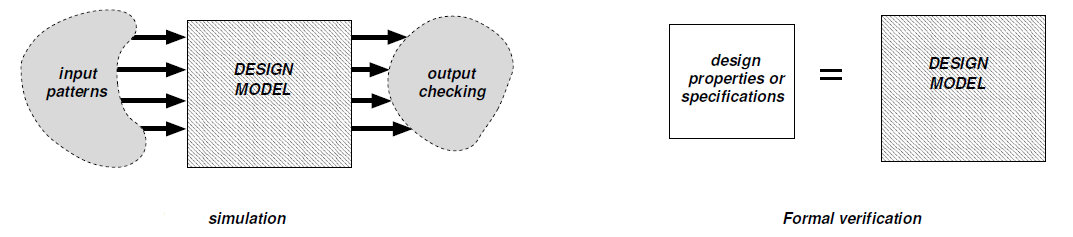
\includegraphics[width=\textwidth]{images/sim_vs_formal.PNG}
	\caption{On the right, a representation of the verification process by Simulation. Stimuli are applied to the DUV inputs and the output behaviour is checked. On the left, Formal Verification checks the DUV against a series of properties that describe the specified behaviour. \cite{thesis-formal}} \TLSAY{Good picture}
	\label{fig:sim-vs-formal}
\end{figure}

The idea of having mathematical proof of the soundness of a design, i.e. the implemented design corresponds to the specification, suggests complex work for the designer, or verification engineer. However, formal verification tools combine three main elements to provide the proof. It comprises proof methods, such as SAT-solving, some specific language, like propositional logic, and models, for example Finite State Machines (FSM). The designer must describe the system as a set of properties and provide them to the tool, which in turn will check if they hold for the RTL implementation. This formal method is also known as property checking. 

Property checking consists of heaving a set of properties describing the specified behaviour of the system and checking whether they can be proved, or checked, for the RTL design.  Therefore, it can be inferred that the RTL description design satisfies the specifications. 

The first step towards having a set of properties is to describe the specified design in an operational view, which can be divided into operations. Each operation represents a specific piece of functional behaviour in finite time interval of the DUV, and can be defined as follows:

\begin{itemize}
    \item Starting important state;
    \item Trigger condition;
    \item Ending important state;
    \item Output behaviour.
\end{itemize}

In other words, an operation describes the behaviour when the design is at a specific important state and a triggering condition happens. Then, the operation defines to which important state the design should go, as well the sequential output behaviour. 

Important states comprise the determination of values for the controls registers of the design. For this reason, they can be also referred as control states. Between the starting state and the ending state, the operation can pass through several non-important states that describe the data path of the design. The triggering condition usually refers to a sequence of inputs, but it can also be a control register having a specific value.

The idea of the operational view is to have a chain of operations that covers the full behaviour of the system. Thus, the end of an operation represents the beginning of other(s). In addition, parallel behaviour can be represented as parallel operations. Examples of operations for a design could be: a read or a write to memory or register file, waiting upon the arrival of a request signal, and the execution of an instruction in a processor.

After specifying the operational view of the design, each operation must be described as a property, or a set of properties, that capture its functionality. In practice, these properties can be written using, for example, System Verilog Assertion (SVA), Property Specification Language (PSL), or even commercial property languages such as ITL \cite{onespin}. A representation of a typical property cab be seen if Fig.~\ref{fig:property}.

\begin{figure}[htb!]
    \begin{lstlisting}
    property accept_request is
    assume:
        at t: state == S1;
        at t: request_i == 1;
    
    prove:
        at t+3: state == S2;
        at t+3: ack_o == 1;
    end property;
    \end{lstlisting}
    \caption{Example of a property that checks the behaviour for a request signal acknowledgement. At an arbitrary time $t$ the circuit is at state $S_1$ and a request signal arrives at the input port $request\_i$. At time $t+3$ the circuit should be at state $S_2$ and an acknowledgement signal is set at the output port $ack\_o$.}
    \label{fig:property}
\end{figure}

The two main parts of a property are the assumptions and commitments. The assumption part characterizes the starting important state and the triggering condition for the operation to be considered. The commitment part depicts the resulting behaviour if the operation is triggered, i.e. outputs description and ending state. A simplified way to represent a property is through a logical implication, Fig.~\ref{fig:a_impl_b}. If a set of assumptions are evaluated as $true$, then the commitments should also be evaluated as $true$ in order to make the property hold. An insight about how verification tools check operational properties is given on Sec.~\ref{subsection:ipc}. Before that, a brief introduction about finite state machines and SAT-solving is presented.

\begin{figure}[htb!]
    \begin{center}
        $a \longrightarrow b$
    \end{center}
    \caption{Logical implication operation where a implies b.}
    \label{fig:a_impl_b}
\end{figure}

\subsection*{Finite State Machine}

A Finite State Machine (FSM) is a deterministic and discrete model of computation that can be, among other applications, used to model a digital circuit. The definition of an FSM is given as follow:

\begin{itemize}
    \item[] $S$: a finite set of states;
    \item[] $s_{0}$: an initial state such that  $s_0 \in S$;
    \item[] $X$: a set of allowed input symbols, input alphabet;
    \item[] $Y$: a set of allowed output symbols, output alphabet;
    \item[] $\delta$: $S \times X \to S$ is a transition function;
    \item[] $\lambda$: $S \times Y \to Y$ is an output function.
\end{itemize}

There are two types of FSM, Mealy and Moore. The aforementioned definition refers to the Mealy type machine. The Moore type only differs on the output function which depends only on the current state $\lambda$: $S \to Y$.

Modelling an electrical circuit as an FSM means that each state of the state machine will correspond to a state of the circuit, i.e. a specific set of values for its control registers. A change of state, determined by the transaction function, and outputs, determined by the output function, will happen upon a change at the inputs. Fig.~\ref{fig:mealy_circuit} depicts a sequential circuit modelled from a Mealy machine.

\begin{figure}[htb!]
	\centering
	
\includegraphics[width=10cm]{images/mealy_circuit.png}
	\caption{Circuit model for a Mealy machine. The combinational circuit models the transition function $\delta$ and output function $\lambda$. The control registers model the state information.}
	\label{fig:mealy_circuit}
\end{figure}

\subsection*{SAT- Solving}

The propositional satisfiability problem, or simply SAT, is the problem of determining if a propositional formula, or Boolean expression, is $satisfiable$, i.e. if it can be evaluated as $true$ for some value combination for its variables. If there is no such combination, and the formula always evaluates to $false$, it is called $unsatisfiable$. 

Considering the formula in Fig.~\ref{fig:a_impl_b}, it is equivalent, and it can be converted, to the formula in the Fig.~\ref{fig:not_a_or_a_and_b}. This expression is $satisfiable$ because it evaluates to $true$ if $a$ is $false$ or if both $a$ and $b$ are $true$. This toy example illustrates how a general property could be converted into a Boolean expression and how SAT-solving could test its satisfiability.

\begin{figure}[htb!]
    \begin{center}
        $\neg a \lor a \land b$
    \end{center}
    \caption{Boolean expression equivalent to logical implication $a \longrightarrow b$.} \TLSAY{Why not not(a) or b ?} 
    \label{fig:not_a_or_a_and_b}
\end{figure}

\subsection{Interval Property Checking}
\label{subsection:ipc}

Interval Property Checking (IPC) is a formal method to prove an operational property for a design \TLINS{startign from a arbitrary time point ... and with an arbirtrary but fixed length}\TLDEL{at an arbitrary time interval}\TLSAY{Arbitrary time interval is wrong. The time interval is exactly given by time point and length}. Let us consider the sequential circuit in Fig.~\ref{fig:mealy_circuit} and a property that has its starting state at time $t$, and its ending state at time $t+3$, like the one in Fig.~\ref{fig:property}. The sequential circuit could be then converted into combinational by using the unrolling technique, Fig.~\ref{fig:unrolled}. The number of “unrolled circuits” will depend on the time interval of interest. In this case $[t, t+3]$.

\begin{figure}[htb!]
	\centering
	
\includegraphics[width=\textwidth]{images/unrolled_circuit.png}
	\caption{Unrolled circuit model for IPC. The unrolled circuit is converted into a Boolean expression which is used to check satisfiability.}
	\label{fig:unrolled}
\end{figure}

The variables from the “unrolled circuit” are then used to describe the property as a Boolean expression. Finally, the SAT-solving tool can evaluate whether the property is $satisfiable$ or not. In other words, IPC proves operational properties by constructing a combinational circuit for the design and solving a SAT problem for it. 

IPC is considered an unbounded model\TLSAY{not true} checking method because its time interval of interest can start at an arbitrary time point. It means that it does not start necessarily from the initial state of the circuit. The equivalent Boolean expression for the unbounded circuit from St to St+n is negated so that it cannot evaluate to $true$. If the SAT-solving tool finds a variable combination that evaluates the formula to $true$ it means that a failure was found. In other words, the property holds for the design if the expression is $unsatisfiable$ \TLSAY{dont use math env. for text just use textit}, otherwise, the respective variables combination that make the expression $satisfiable$ are presented by the tool as a counter-example.

Finding a counter-example does not necessarily means that there is a bug in the design. In fact, there could be a fault \TLSAY{its not a fault on the computational model ... it's just a spurious counter example} on the computational model. Since the starting state \TLREP{St}{$S_t$} can be arbitrary, it is important that it represents a reachable state of the design. During the verification process, when a property fails, the generated counter-example must be analysed in order to identify if it represents a possible scenario for the design of if it is a spurious counter-example, i.e. \TLREP{St}{$S_t$} \TLSAY{change everywhere} represents an unreachable state.

The reachability problem for IPC can be addressed by the concept of invariants. An invariant is a set of states that contains all states reachable from its own states. Let us consider for example a State Machine M. An invariant W of M is any set of states of M that contains all states reachable from W. In this sense, if a property holds for a state St E W, and W contains the initial state, the property holds for every reachable state of the system. Thus, if a spurious counter-example is generated by the tool, reachability information should be added to St as invariants. In practice, the assumptions of the property have to be constrained in order to represent a reachable state. 

\subsection{Gap-free verification}

As previously mentioned, the justification for using Formal Techniques to verify a digital design lies on its potential to achieve completeness \TLSAY{Completeness is not defined upon this point and its pretty special thing. You should express what completeness means in words upon the point of definition. Same is valid for gap-free. This also counts for your introduction}. In order to understand this concept better, let us first consider the notion of termination criteria. Conventional verification approaches have their termination criteria relying on the verification plan. Simulation based verification needs a verification plan that will result in a test bench that covers all possible \TLDEL{behaviour} scenario\TLINS{s}. This, of course, is very hard to \TLREP{achieve}{reach} for many designs even using random stimuli techniques. As for assertion-based verification (ABV), the hazard is on determining when the assertions written are enough to comprise the specified behaviour. Formal verification will have its termination criteria anchored on the concept of completeness.

A property set is said to be complete if it has a property, or subset of properties, describing each operation of a design, hence completely describing the specified behaviour of the system. With this, there is no gap between the RTL implementation and specifications, so the name \TLSAY{parse error} gap-free verification. \TLSAY{gap-free is a OneSpin trademark, you should reference their website}

\TLSAY{In text we imagine that a citation is the same as a person} \cite{paper-gapfree} defines a set of operation properties as complete, if it uniquely describes the output behaviour of a circuit according to determination requirements. These determination requirements specify which outputs and states variables are to be determined in each operation. To establish\TLSAY{wrong word ... check?} if a set of property is complete, the following completeness tests can be performed \cite{guide-onespin}:

\begin{enumerate}[A.]
    \item \textbf{The Case Split Test:} This test checks whether the chain of operations is comprised by the property set. Therefore, for each state reached by a property, there must be a property starting at this state for every input combination.
    \item \textbf{The Successor Test:} The successor test checks if the chain of properties is uniquely determined. In this sense, for every property the test check if each succeeding property is uniquely determined for its input trace.
    \item \textbf{The Determination Test:} This test will check the determination requirements. It verifies if the outputs and determined state registers, also referred as visible registers, are uniquely determined for all operations.
    \item \textbf{The Reset Property:} The reset test checks the initialization of the design. After the reset sequence, the design should end at a unique important state, and have determined all the signals according to the determination requirements.
\end{enumerate}


\section{Property-Driven Design}

\subsection{SystemC-PPA Model}

\subsubsection{PPA overview}

\subsubsection{SystemC-PPA}

\subsection{The PDD flow}

\subsection{DeSCAM}

\subsection{Completeness with S2QED}



\newpage
% ----------------------------------------------------------
% Verification of Pipelined Processors
% ----------------------------------------------------------
\chapter{Verification of Pipelined Processors}

This chapter presents a brief discussion on how IPC can be used to verify a pipelined processor. First, the concept of \textit{Pipelining} is reviewed with its main characteristics in Sec.~\ref{section:pipe-overview}. Then, an introduction on how to create an operational description of a pipelined processor along with a property example is presented in Sec.~\ref{section:ipc-pipe-processor}. Next, the notion of completeness for pipelined processors is discussed, including an introduction to the \SSQED{} approach, in Sec.~\ref{section:s2qed}. Finally, a discussion about the PDD method for Pipelined Processors is presented in Sec.~\ref{section:pdd-pipe-processor}.  

\section{Overview of Pipelined Processors}
\label{section:pipe-overview}

\textit{Pipelining} is a technique used to allow overlapping execution of instructions in a single core of a processor \cite{book-comp-org}. Instead of having instructions executing one after another in a sequential manner, the execution path for the instruction is divided into steps, called \textit{pipeline stages}. Thus, multiple instructions can overlap in time, each one executing in a different stage of the pipeline, Fig.~\ref{fig:pipe-example}.

\begin{figure}[htb!]
	\centering
	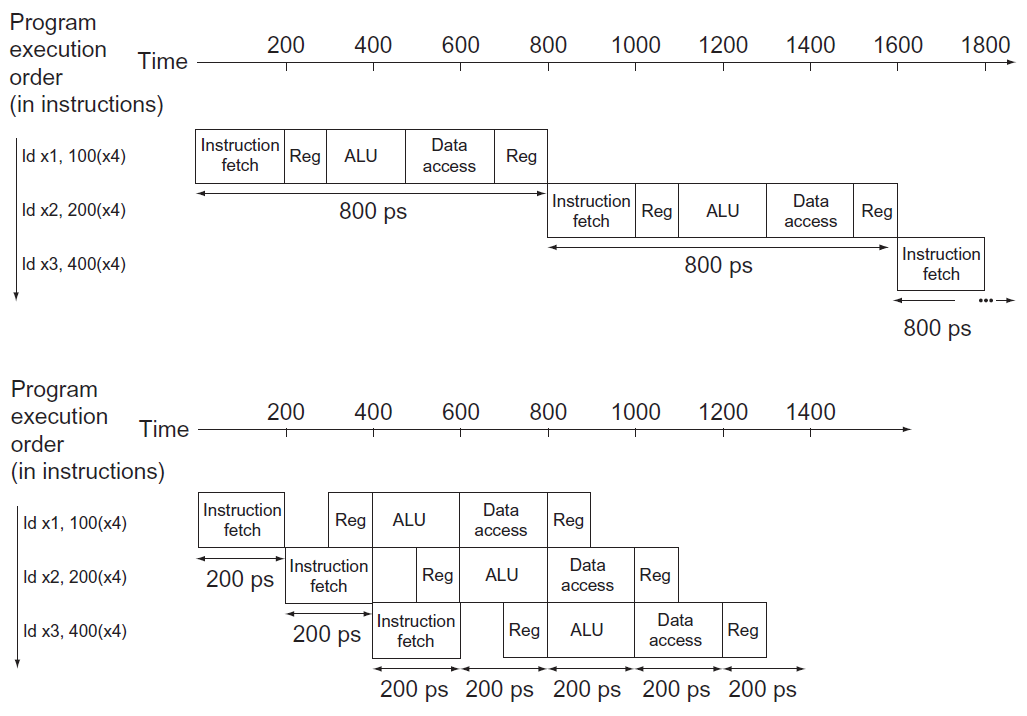
\includegraphics[width=0.85\textwidth]{images/pipeline-example.PNG}
	\caption{Illustration of the execution of instructions in a nonpipelined processor (top) versus pipelined execution (bottom). The \textit{ld} instruction loads data from the memory into a register in the processor register file. In this example, memory \textit{stalls} are not considered. (Reprinted from \cite{book-comp-org})}
	\label{fig:pipe-example}
\end{figure}

Since different types of instructions have very similar execution \textit{steps}, each step on the data path can be turned into a pipeline stage. For example, a common partition adopted in different pipelined processor implementations is: 

\begin{itemize}
\item Instruction Fetching (\textit{IF}): fetches a new instruction from memory to feed the pipeline;
\item Instruction Decoding (\textit{ID}): decodes instruction \textit{opcodes} and reads its operands from the register file;
\item Execution (\textit{EX}): executes the instruction operation. Usually associated with ALU operations;
\item Data Access (\textit{MEM}): performs \textit{read} and \textit{write} operations with data memory;
\item Write back (\textit{WB}): writes back the operations results or loaded data from data memory.
\end{itemize}

Certainly, each processor can have its own pipeline implementation, but they usually constitute some variation of the five presented stages.

One main advantage of pipelining is increasing the instruction \textit{throughput}, the amount of processed data per time unit. This advantage is illustrated in Fig.~\ref{fig:pipe-example}. In this example, a single \textit{load} instruction takes 800\,ps in a nonpipelined processor. Considering a pipelined processor with the five aforementioned stages, and with each stage taking 200\,ps, the three \textit{load} instructions execute in 1400\,ps, in contrast to the 2400\,ps needed for the nonpipelined processor. In this example, of course, possible \textit{stalls} caused by waiting for data memory are not considered for simplicity reasons. 

\section{Property Checking for Pipelined Processors}
\label{section:ipc-pipe-processor}

In order to verify the design by property checking, the processor behaviour has to be described in term of operations, see Sec.~\ref{section:formal-verification}. There are many ways to achieve that, but one simple and intuitive way is to consider an operation as the complete execution of an instruction through all the pipeline stages. This operational description is more intuitive because the behaviour of each instruction is already specified in the \textit{Instruction Set Architecture}~(ISA) of the corresponding implemented processor, and it is simpler than specifically describing different combinations of instructions at different pipeline stages at time.

Since every operation starts and ends at an \textit{important state}, a common pipeline stage can be chosen as the initial and final state. As an example, one may consider the \textit{IF} stage as the \textit{important state} and that every operation starts being fetched and ends when the next instruction is fetched. In practice, when the \textit{Instruction Under Verification}~(IUV) moves from \textit{IF} to \textit{ID}, the next instruction is already fetched.

A complete set of properties needs to prove all \textit{outputs} and \textit{visible registers} at all times, see Sec.~\ref{subsection:notion-completeness}, according to determination requirements. For this operational description of pipelined processor, one property will prove \textit{outputs} and \textit{visible registers} corresponding to each pipeline stage. Consider the property in Fig.~\ref{fig:ex-add-ppt}. It depicts an example of a property proving the \textit{ADD} instruction in a 4-stages pipeline processor. The \textit{Program Counter} (PC) is proven only at the \textit{ID} stage, $t\_ID$. This does not compromise the completeness if there is always a property proving PC at all times. For example, at $t\_IF$ the previous instruction is at the \textit{ID} stage and proves the PC, and at $t\_EX$ is the instruction succeeding the IUV which is at the \textit{ID} stage proving the PC.

\begin{figure}[htb!]
    \begin{lstlisting}
    property ADD;
    assume:
        //conceptual state
        at t_IF: conceptual_state;
        at t_IF: empty_pipeline;
    
        //Trigger
        at t_IF: instr_type(fetched_instr) == ADD;
    prove:
        at t_ID: conceptual_state;
        at t_ID: PC == PC_at_t_IF + 4;
    
        at t_EX: ALU_oper_a == getOperA(fetched_instr);
        at t_EX: ALU_oper_b == getOperB(fetched_instr);
        at t_EX: ALU_result == ALU_oper_a + ALU_oper_b;
        
        at t_WB: regile_wb == ALU_result;
    
        at t_end: REGFILE(reg_dest) == ALU_result;
    end property;\end{lstlisting}
    \caption{Example of a property describing the execution of the \textit{ADD} instruction in a pipelined processor.}
    \label{fig:ex-add-ppt}
\end{figure}

In the example property for an \textit{ADD} instruction in Fig.~\ref{fig:ex-add-ppt}, the processor is in a state called \textit{conceptual\_state} at $t\_IF$, line 4. This conceptual state corresponds to a state where the processor is ready to fetch a new instruction. When the IUV is at the \textit{ID} stage, the processor should be again at the conceptual state and ready to fetch a new instruction, line 10. Back to the assumptions, the property states that the fetched instruction is of type \textit{ADD}. In the commitments, the visible register PC is proved to be incremented by four at $t\_ID$. At $t\_EX$, the property proves that the ALU receives the right operands and computes the right result. At $t\_WB$, the right result is sent back to the register file. Finally, at $t\_end$, the destination register in the register file holds the right computed result.

A property set that covers the \textit{reset} behaviour and has one property for every possible instruction in the ISA will pass the completeness tests for successor, determination, and reset (see Sec.~\ref{subsection:notion-completeness}). However, the case-split test will not hold. This is because the properties referred so far assume that the IUV execution is not influenced by any other instruction in the pipeline. Line 5 in the listing of Fig.~\ref{fig:ex-add-ppt} assumes that the pipeline is empty when the IUV is fetched. Obviously, in practice this will hardly be the case. In order to overcome this problem, an approach called \SSQED{} \cite{paper-symbolic} can be employed. The next section presents an overview of this approach.

\section{Completeness with \SSQED{}}
\label{section:s2qed}

\SSQED{} \cite{paper-symbolic} is a verification approach based on a bounded model with symbolic initial state. It offers a proof that the execution of each instruction is independent of its \textit{program context}. In other words, each instruction executes independently of other instructions currently in the pipeline. 

Errors in hardware design are often called “\textit{bugs}” or “\textit{logic bugs}”. In \cite{paper-gapfree}, these errors are defined as a deviation of the implementation’s behaviour from the specification. Also in \cite{paper-gapfree}, two categories of logic bugs are presented:

\begin{enumerate}
\item Single-instruction bug: it is defined when the \textit{opcode} and the operands of the IUV causes an error in all program contexts, i.e. independently of all previously executed instructions.
\item Multiple-instruction bug: it is defined when it is not a single-instruction bug and there exists an instruction \textit{opcode}, a set of operands and a program context such that the execution of the IUV leads to an error.
\end{enumerate}

The property set presented so far, composed with properties like the one in Fig.~\ref{fig:ex-add-ppt}, is able to identify single-instruction bugs since they are independent of the program context. Therefore, the \textit{empty\_pipeline} assumption will not interfere on finding these types of errors. On the other hand, this assumption will mask multiple-instruction bugs as they require specific instruction sequence scenarios in order to occur.

In order to exemplify a multiple-instruction bug, consider a \textit{read-after-write} hazard. This hazard happens, for example, when an instruction \textit{reads} a register that is written by its immediate previous instruction. In this case, considering the same 4-stages pipeline, the register value is read before the "write to the register file" operation is complete by the previous instruction. To avoid an error, pipelined processors implement a mechanism called \textit{forwarding}. This mechanism forwards the value that is going to be written in the register file to previous pipeline stages, so it can be used by the following instruction if needed. A bug in the forwarding structure is considered a multiple-instruction bug as it does not depend only on the IUV, but in previous instruction fed into the pipeline. 

The \SSQED{} approach covers multiple-instruction bugs by assigning one same instruction, at an arbitrary time point, to execute in two \textit{identical} and \textit{independent} instances of the processor under verification. The computational model of the \SSQED{} approach is depicted in Fig.~\ref{fig:s2qed-model}.

\begin{figure}[htb!]
	\centering
	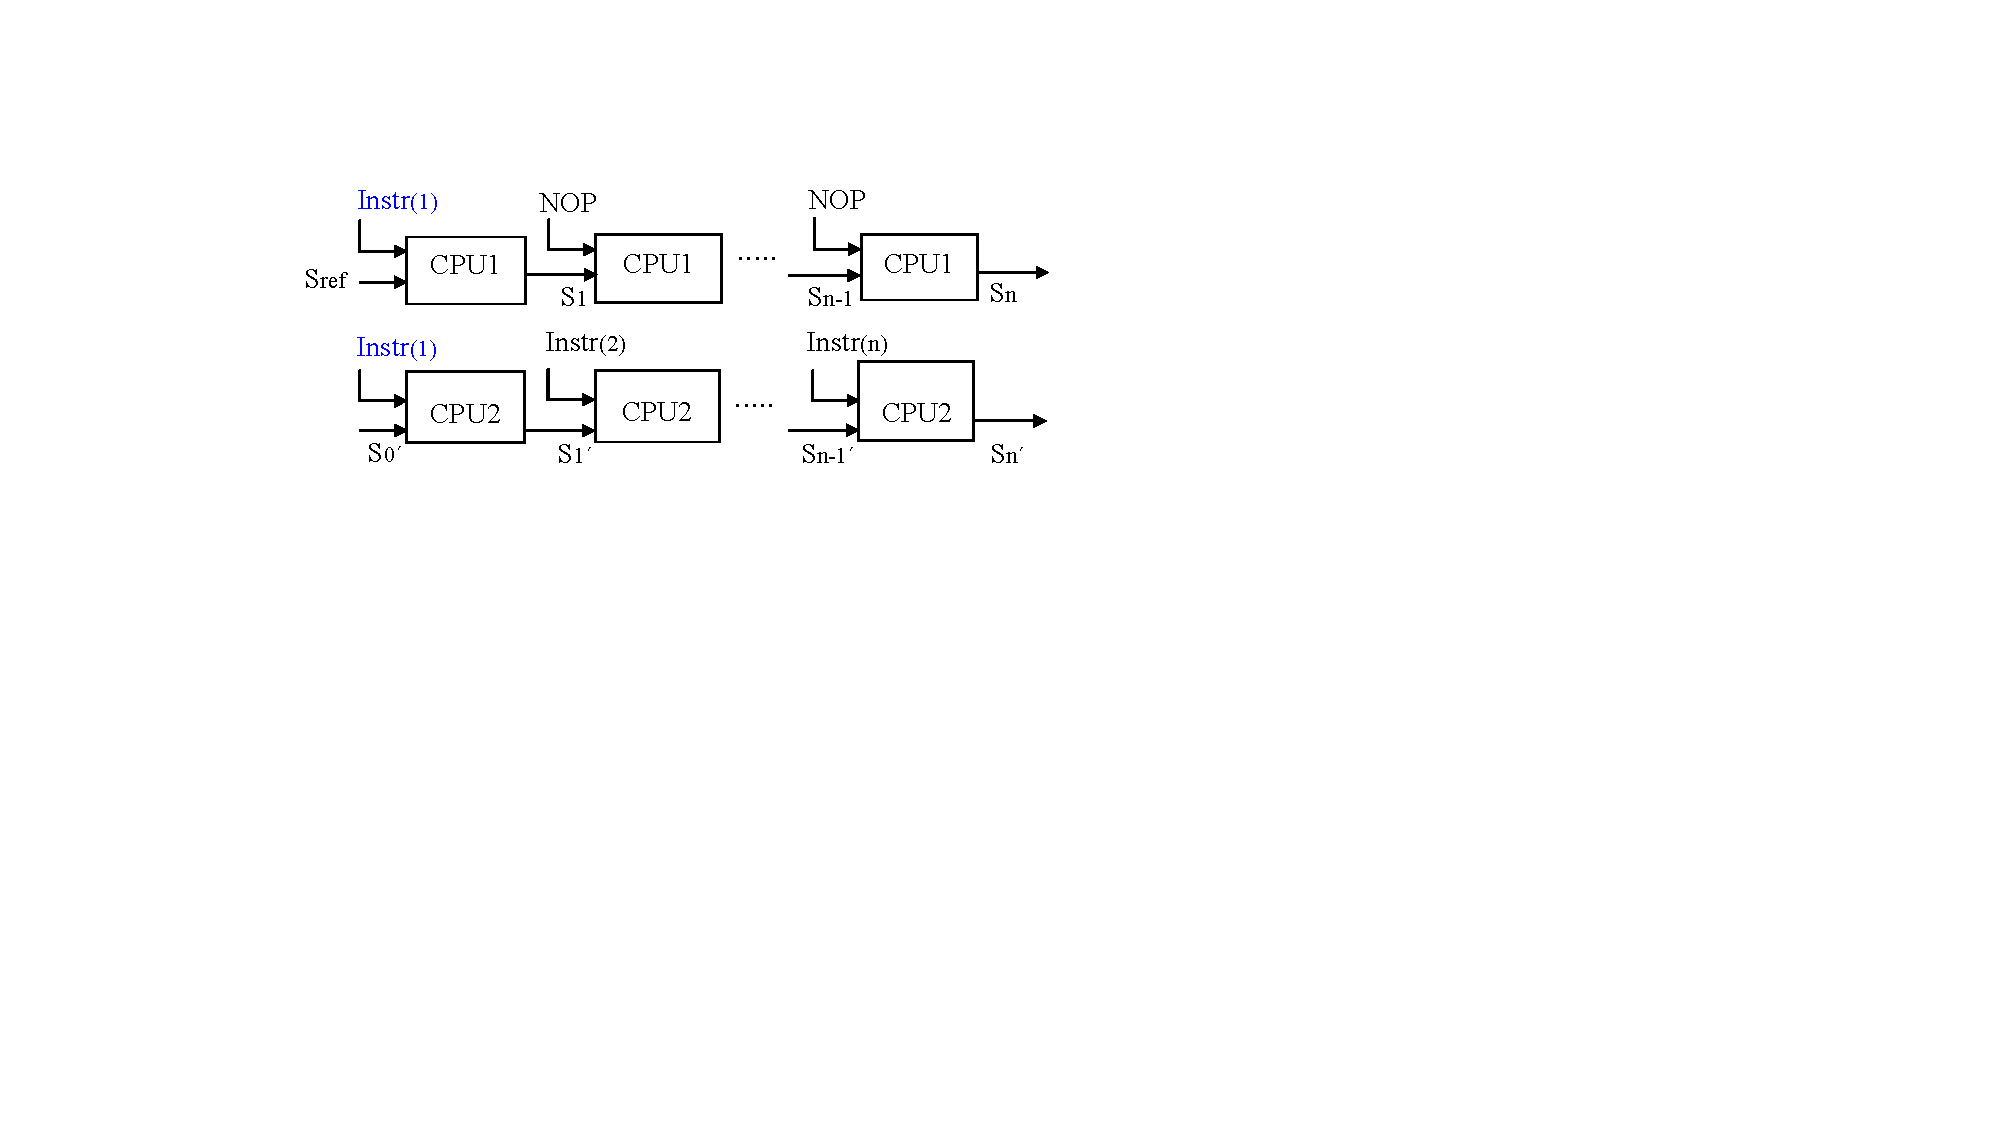
\includegraphics[width=0.7\textwidth]{images/s2qed_model.pdf}
	\caption{\SSQED{} computational model. Both constrained and unconstrained instances, \textit{CPU1} and \textit{CPU2} respectively, execute the same IUV. (Reprinted from \cite{paper-gapfree})}
	\label{fig:s2qed-model}
\end{figure}

The first CPU instance, in the same manner as the CPU model considered so far, is constrained to execute the IUV in an empty pipeline. The second CPU instance is unconstrained to execute an arbitrary sequence of instructions. The only restrictions for the second CPU instance are that it fetches the same instruction as the first instance at time $t$, and they both are consistent. This required consistency, named \textit{QED-consistency}, is defined in \cite{paper-gapfree} as follows:

\begin{quote}
     \textit{"In the \SSQED{} computational model, the two CPU instances are QED-consistent at a time $t$, if the corresponding architectural state elements of both instances at time point $t$ hold the same values."}
\end{quote}

For this \SSQED{} computational model, the SAT-Solving tool will compare the execution of the IUV in the constrained empty pipeline of the first CPU instance with all the scenarios for the unconstrained execution of the IUV in the second CPU instance, including the context where the multiple-instruction bugs appear and propagate. The listing on Fig.~\ref{fig:ex-s2qed-add-ppt} shows an example of an \SSQED{} property for an \textit{ADD} instruction.

\begin{figure}[htb!]
    \begin{lstlisting}
    property S2QED_ADD;
    assume:
        // constraints on CPU1
        at t_IF: cpu1_conceptual_state;
        at t_IF: cpu1_empty_pipeline;
        during [t_IF+1, t_WB]: instr_type(cpu1_fetched_instr) == NOP;
    
        // same IUV
        at t_IF: cpu1_fetched_instr == cpu2_fetched_instr;
        at t_IF: instr_type(cpu1_fetched_instr) == ADD;
    
        // QED consistent registers
        at t_WB: qed_consistency_registers();
    
    prove:
        at t_end: qed_consistency_registers();
        end property;\end{lstlisting}
    \caption{Example of a \SSQED{} property describing an \textit{ADD} instruction as the IUV.}
    \label{fig:ex-s2qed-add-ppt}
\end{figure}

Lines 4 and 5 of the property in Fig.~\ref{fig:ex-s2qed-add-ppt} constrain the \textit{CPU1} instance to be on the conceptual state and have an empty pipeline. The assumption in line 6 constrains the \textit{CPU1} to fetch only \textit{NOP} instructions after fetching the IUV. This assumption is not crucial to prove the model, however, it reduces unnecessary complexity for the SAT-solving tool. The assumptions on lines 9 and 10 will bind the IUV in both CPU instances to be the same and of type \textit{ADD}. Finally, the last assumption on line 13 comprises the QED-consistency, which is also proven on the commitment on line 16.

The macro function \textit{qed\_consistency\_registers()} expresses the Boolean function shown in Eq.~\ref{eq:consistency-register}. It characterizes the QED-consistency register state for a processor with $N$ registers on its register file.

\begin{equation}
    qed\_consistency\_registers := \,\, \bigwedge_{i = 0}^{N-1} \left(R^i_{cpu1} = R^i_{cpu2}\right)
    \label{eq:consistency-register}
\end{equation}

The consistency between the two CPU instances is the key for accomplishing completeness solving the case-split test. The \SSQED{} computational model guarantees a consistent result of every operation between both instances. Therefore, proving the case-split test for one of the instances is sufficient.

The case-split test is easy to satisfy for a set of \SSQED{} properties, since every possible instruction sequence is implicitly considered on the \textit{CPU2} instance. For a formalism on how the case-split test is proven on a \SSQED{} property set, the reader may refer to \cite{paper-gapfree}.

\section{PDD for Pipelined Processors}
\label{section:pdd-pipe-processor}

The Property-Driven Design approach, see Sec.~\ref{section:PDD}, generates operational properties from an ESL design described in SystemC-PPA in order to prove that the later implemented RTL design is sound with respect to the ESL. The SystemC-PPA description is a sequential model from which the extracted operations represent transitions between important states. 

A pipelined processor will have its operations overlapping in time, for each operation represents an instruction executing throughout the pipeline stages. Consequently, while the ESL model describes the behaviour of instructions of a program executing sequentially one after another in the processor (see the execution on top of Fig.~\ref{fig:pipe-example}) the RTL implements the pipeline where an instruction starts executing before the previous one is completed. This concurrent behaviour is shown on the bottom of Fig.~\ref{fig:pipe-example}.

If the ESL model does not describe the concurrent execution of operations, the generated PPA will not match the pipeline implemented in the RTL. In practice, the \textit{DeSCAM} tool (see Sec.~\ref{subsection:PDD-flow}), that generates the properties, derives the important states from communication transactions in the DUV, so the operations represent the data manipulation between communication. 

Let us consider the 4-stage pipeline processor defined in this chapter with two communicating interfaces. One memory interface to fetch instructions and the other for communication with the data memory. Fig.~\ref{fig:ppa-seq} shows the PPA extracted from the sequential SystemC-PPA description of the processor. 

\begin{figure}[htb!]
	\centering
	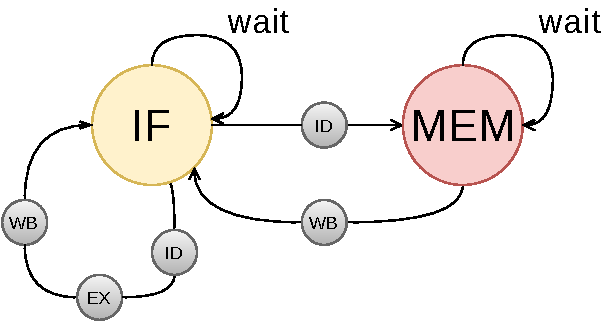
\includegraphics[width=0.6\textwidth]{images/PPA_old.pdf}
	\caption{PPA for a sequential SystemC-PPA processor description.}
	\label{fig:ppa-seq}
\end{figure}

The bigger circles in the PPA of Fig.~\ref{fig:ppa-seq} represent important states where there is some transaction with a communication port, while the smaller circles represents unimportant states. There are two important states, the \textit{IF} state that communicates with the instruction memory, and the \textit{MEM} state that communicates with the data memory.

The listing of Fig.~\ref{fig:ex-pdd-add-ppt} shows an example of a property generated for an \textit{ADD} instruction from a sequential ESL. The time $t$ corresponds to the fetching time, and the time $t\_end$ to the time point after the write back, $t+4$. The property is triggered when the CPU is ready to fetch, \textit{conceptual\_state}, and a new instruction of type \textit{ADD} is fetched. At $t\_end$, after the \textit{ADD} instruction is completely executed, the commitments prove that the right result is written to the right destination register.

\begin{figure}[htb!]
    \begin{lstlisting}
    property PDD_ADD;
    assume:
        at t: conceptual_state;
        at t: instr_type(fetched_instr) == ADD;
    prove:
        at t_end: conceptual_state;
        at t_end: PC == PC_at_t + 4;
        at t_end: REGFILE(reg_dest) == ADD_result;
        
        //intruction memory interface
        during [t+1, t_end-1]: instr_req_out_notify == false;
        at t_end: instr_req_out_notify == true;
        
        //data memory inteeface
        during [t+1, t_end]: data_req_out_notify == false;
    end property;\end{lstlisting}
    \caption{Example of a property for the \textit{ADD} instruction generated from a sequential PPA.}
    \label{fig:ex-pdd-add-ppt}
\end{figure}

It is important to notice that the request signal to fetch a new instruction is only asserted at the time point $t\_end$, being set to false during the whole instruction execution time. Similarly, the request signal for the data memory is de-asserted all the time since the \textit{ADD} instruction does not communicate with the data memory at any time. As a result, a set with $n$ properties corresponding to the $n$ instructions of the processor ISA will not hold for the RTL design. One problem can be easily spotted in this example. Consider the operation property for a \textit{LOAD} instruction, while the \textit{ADD} property tries to prove that the \textit{data\_req\_out} signal is always false, the \textit{LOAD} instruction tries to prove that the same signal is set to true during the memory phase.

Two approaches could be considered in order to apply the PDD flow for the design of a pipelined processor. First, the designer can redesign the ELS description so that it reflects the pipeline concurrent RTL behaviour. In this case, the ESL abstraction is lost because RTL implementation details are replicated at the ESL model. The second alternative is refining the pipeline within the macros for the generated instructions. Once again, the designer would have to replicate part of the RTL implementation, this time during the refinement of the macros. 

For both approaches, additional effort by the designer is required, which mitigates the goal of applying the PDD method, that is to accelerate the design process. Chapter~\ref{chapter:algorithm} presents how the PDD approach can be extended for pipelined processors by introducing small changes at the SystemC-PPA, and proposes an algorithm that can be used to convert the generated \textit{DeSCAM} properties into a property set that matches the pipeline concurrent behaviour. 


\newpage
% ----------------------------------------------------------
% The Pipeline Algorithm
% ----------------------------------------------------------
\chapter{The Pipeline Algorithm}
\label{chapter:algorithm}

The current chapter presents how the PDD flow can be extended in order to support the design of pipelined processors in Sec.~\ref{section:extend-pdd}. Sec.~\ref{section:pipe-algorithm} introduces the Pipeline Algorithm to generate a set of Pipeline Properties. Finally, in Sec.~\ref{section:plugio-s2qed-top}, a plugin for \textit{DeSCAM} to assist on the \SSQED{} environment setup is presented. 

\section{Extending the PDD flow for Pipelined Processors}
\label{section:extend-pdd}

The Property-Driven Design flow presented on Sec.~\ref{subsection:PDD-flow} can be extended to help the hardware designer to deal with pipelined processors. The original PDD flow is depicted on the left side of Fig.~\ref{fig:new-pdd-flow}. On the right side, an extended PDD flow is presented with two additional steps that are included to support pipelined processors: insert stages and pipeline algorithm. 

\begin{figure}[htb!]
	\centering
	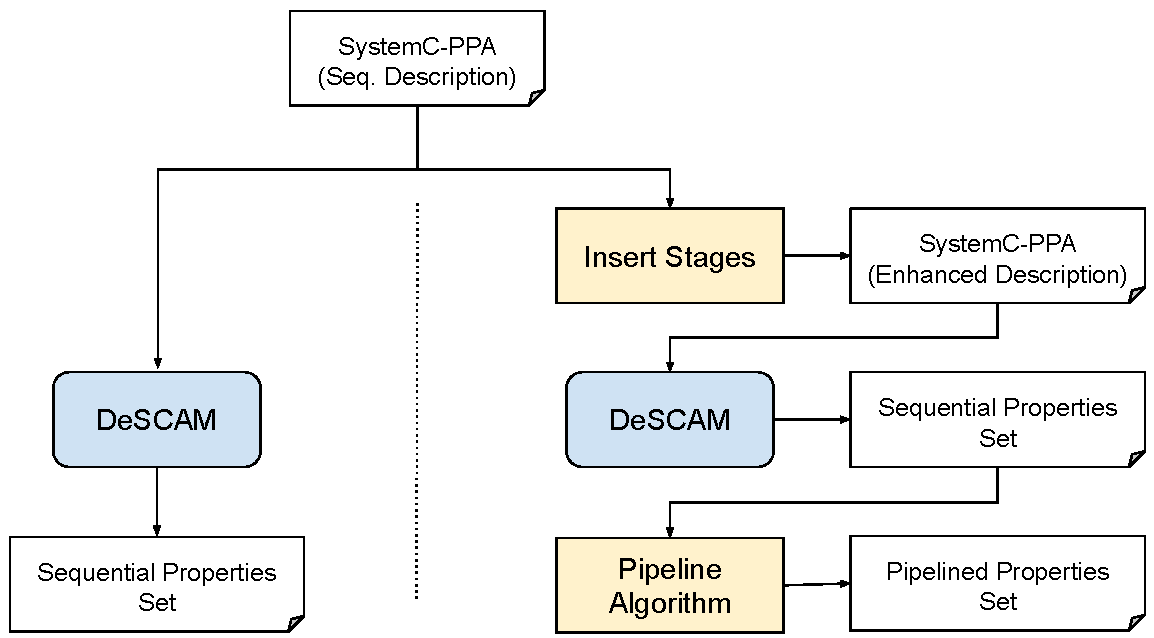
\includegraphics[width=0.85\textwidth]{images/new_pdd_flow.pdf}
	\caption{On the left, property generation with \textit{DeSCAM} for the original PDD flow. On the right, extension of the PDD flow to better support of pipelined processors.}
	\label{fig:new-pdd-flow}
\end{figure}

In the same manner as the original flow, the extended PDD flow starts with a description at the architectural-level, which is PPA compliant. Before applying the description to \textit{DeSCAM}, the SystemC-PPA model is modified to include information about the pipeline behaviour resulting in an enhanced PPA description. This description can be applied to \textit{DeSCAM} which will generate a sequential property set of \textit{micro properties} (to be detailed later in this section). Finally, the \textit{Pipeline Algorithm} can merge the \textit{micro properties} generating a property set with \textit{pipeline properties}.

The \textit{Insert Stages} phase allows the designer to include information about the desired pipeline structure into the SystemC-PPA model. It is important to emphasise that the designer does not have to translate the concurrent pipeline behaviour from the RTL implementation into the ESL model. The designer needs simply to include information about the desired pipeline stages at the appropriate points. This is done by calling the function \textit{insert\_state()} at the points in the data path of the ESL model corresponding to each pipeline stage. This function call will not influence on the sequential behaviour of the simulation for the model at the system-level.

The \textit{insert\_state()} function is interpreted by the \textit{DeSCAM} tool as a directive to include an important state in the PPA for that respective position in the code. Without this directive, the important states were only generated for communication calls, which affects the \textit{I/O} behaviour (see Sec.~\ref{subsection:PDD-flow}). Consider the regular PPA in Fig.~\ref{subfig:ppa-seq} extracted from a sequential ESL model without the manually inserted stages. If a call to insert a state for each pipeline stage is used, the resulting enriched PPA such the one in Fig.~\ref{subfig:ppa-pipe-processor} is obtained.

\begin{figure}[htb!]
\centering
\begin{subfigure}[b]{0.45\textwidth}
  \centering
	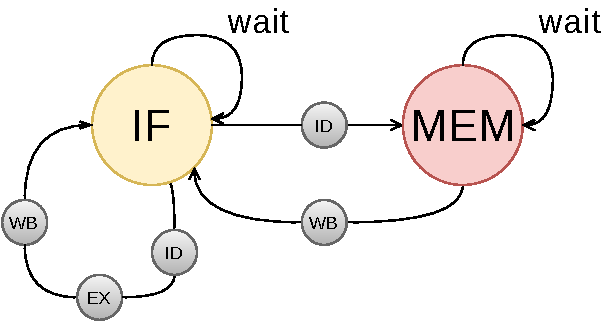
\includegraphics[width=0.9\textwidth]{images/PPA_old.pdf}
	\caption{PPA for regular PDD flow.}
	\label{subfig:ppa-seq}
\end{subfigure}
\hfill
\begin{subfigure}[b]{0.45\textwidth}
  \centering
	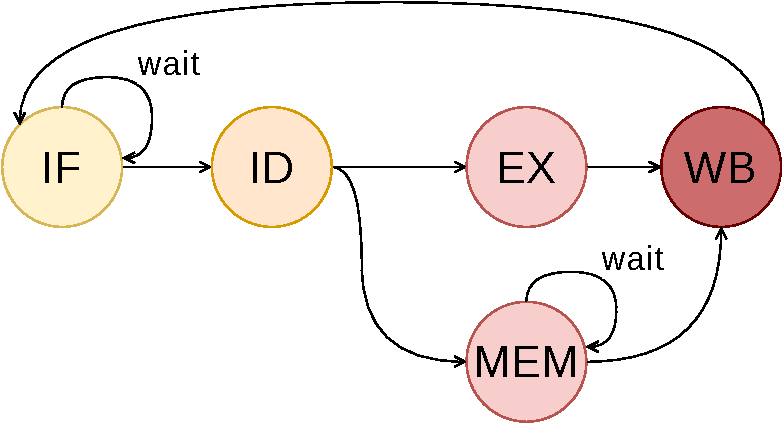
\includegraphics[width=0.9\textwidth]{images/PPA_new.pdf}
	\caption{PPA for extended PDD flow.}
	\label{subfig:ppa-pipe-processor}
\end{subfigure}
\caption{(a) PPA for a sequential SystemC-PPA processor description like in Fig.~\ref{fig:ppa-seq}. (b) Enriched PPA for an enhanced SystemC-PPA processor description with states inserted for each pipeline stage.}
\label{fig:ppa-old-and-new}
\end{figure}

The enriched PPA of Fig.~\ref{subfig:ppa-pipe-processor} derived from an enhanced SystemC-PPA has one important state for each pipeline stage. As a result, the property set generated by \textit{DeSCAM} will also be different. Let us consider an \textit{ADD} instruction for a 4-stage pipeline processor as an example. The property generated by \textit{DeSCAM} for a regular sequential SystemC-PPA description is seen in the listing of Fig.~\ref{fig:ex-pdd-add-ppt}. Since only one important state, for instance \textit{IF}, is present on the execution path of an \textit{ADD} instruction, only one property is generated for describing the behaviour of this instruction. This can be also seen on the PPA of Fig.~\ref{subfig:ppa-seq} where the \textit{ADD} operation corresponds to a single edge starting  and ending on important state \textit{IF}. On the other hand, an \textit{ADD} instruction execution on the enriched PPA of Fig.~\ref{subfig:ppa-pipe-processor} corresponds to four edges. Therefore, four properties will be generated for this single instruction. These operations describing the behaviour between two pipeline stages are named \textit{micro operations}, or \textit{micro properties}. The listing on Fig.~\ref{fig:add-if-id-micro-ppt} shows two examples of micro properties. The property in Fig.~\ref{subfig:add-if-micro-ppt} corresponds to the operation between the \textit{IF} and \textit{ID} stages, and the property in Fig.~\ref{subfig:add-id-micro-ppt} the operation when the IUV goes from stage \textit{ID} to \textit{EX}.

\begin{figure}[htb!]
     \centering
     \begin{subfigure}[b]{\textwidth}
         \begin{lstlisting}
    property PDD_ADD_IF;
    dependencies: no_reset;
    for timepoints:
        t_end = t+1;
    freeze:
        PC_at_t = PC@t;
    assume:
        at t: IF;
    prove:
        at t_end: ID;
        at t_end: PC == PC_at_t + 4;
        at t_end: fetched_instr == instr_in_sig;
        at t_end: operands == getOperandsFromRegFile(fetched_instr);
        during [t+1, t_end-1]: instr_req_out_notify == false;
        at t_end: instr_req_out_notify == true;
        during [t+1, t_end]: data_req_out_notify == false;
    end property;\end{lstlisting}
         \caption{Micro property describing operation from \textit{IF} stage to \textit{ID} stage.}
         \label{subfig:add-if-micro-ppt}
     \end{subfigure}
     \hfill
     \begin{subfigure}[b]{\textwidth}
         \begin{lstlisting}
    property PDD_ADD_ID;
    dependencies: no_reset;
    for timepoints:
        t_end = t+1;
    freeze:
        PC_at_t = PC@t,
        fetched_instr_at_t = fetched_instr@t;
    assume:
        at t: ID;
        at t: getInstrType(fetched_instr) == ADD;
    prove:
        at t_end: EX;
        at t_end: PC == PC_at_t;
        at t_end: fetched_instr == fetched_instr_at_t;
        at t_end: ex_regData == operands.rs1 + operands.rs2;
        at t_end: ex_regAddr == operands.rd;
        at t_end: ex_regWrEn == true;
        during [t+1, t_end]: instr_req_out_notify == false;
        during [t+1, t_end]: data_req_out_notify == false;
    end property;\end{lstlisting}
         \caption{Micro property describing operation from \textit{ID} stage to \textit{EX} stage.}
         \label{subfig:add-id-micro-ppt}
     \end{subfigure}
        \caption{Example of micro properties generated for an \textit{ADD} instruction from an enhanced SystemC-PPA processor description with states inserted to each pipeline stage. The property in (a) refers to the transition between \textit{IF} and \textit{ID} stages, and the property in (b) the transition between \textit{ID} and \textit{EX}.}
        \label{fig:add-if-id-micro-ppt}
\end{figure}

One problem with describing the behaviour of a single instruction with multiple micro properties is the loss of intuitiveness for the designer. It is more natural to describe an instruction behaviour spawning over all pipeline stages. A second problem is that each micro operation generated will describe the behaviour of all \textit{outputs} and visible registers. As discussed in Sec.~\ref{section:pdd-pipe-processor}, this makes the property set impossible to hold because each property, in this pipelined processor context, should prove only the values of interest for the corresponding stage. An example of this problem can be observed in the micro properties of Fig,~\ref{fig:add-if-id-micro-ppt}. The PC behaviour is correctly proven to be incremented in (a) when the IUV is on the \textit{ID} stage. However, in (b), the PC is proven to remain with the same value. This is not true as the PC is normally incremented in every clock cycle as a new instruction is fetched. Another inconsistency refers to the output signal requesting a new instruction, \textit{instr\_req\_out\_notify}. In the  commitments of (b), the signal is proven to be de-asserted, which is not the expected behaviour of a pipeline processor that requests a new instruction every clock cycle when there is no \textit{stall}.

The other additional phase included on the extended PDD flow of Fig.~\ref{fig:new-pdd-flow} is the \textit{Pipeline Algorithm}. This proposed algorithm combines the micro properties referring to a single instruction into a \textit{pipeline property}. This property describes the behaviour of the instruction executing throughout all pipeline stages, similarly to the property shown in the listing of Fig.~\ref{fig:ex-add-ppt}. The Pipeline Algorithm is detailed in Sec.~\ref{section:pipe-algorithm}.

The notion of completeness discussed in Sec.~\ref{section:ipc-pipe-processor} and Sec.~\ref{section:s2qed} still applies. The set of pipeline properties generated by the algorithm represents the set of constrained properties that considers the IUV executing in a empty pipeline. For passing the case-split test and achieving completeness, a set of \SSQED{} properties has to be proven.

Finally, in addition to the HDL template that can be generated by \textit{DeSCAM} in order to assist the designer on the RTL implementation, see Sec.~\ref{subsection:PDD-flow}, a new plugin  for \textit{DeSCAM} was developed in this work. This plugin can be optionally used by the designer to automatically generate a top design in HDL creating the environment to prove the \SSQED{} properties. The plugin is detailed in Sec.~\ref{section:plugio-s2qed-top}.

\section{Generating the Pipeline Properties}
\label{section:pipe-algorithm}

The Pipeline Algorithm proposed in this work converts a property set of micro operations into a set of pipeline properties. Given a processor description at the architectural-level including the information of each pipeline stage by state insertion, the \textit{DeSCAM} tool will generate a sequence of properties for each instruction from the ISA of the processor model. The algorithm will merge the sequence of properties for each instruction into a single pipeline property. 

The listing in Fig.~\ref{fig:sysc-pipe-proc} shows an example of a SystemC-PPA compliant processor description. For simplicity, the presented ESL implementation omits some code such as variable declarations and function implementations. The purpose of this example is to illustrate one possible implementation of a 4-stages pipeline processor at the architectural-level that will be used throughout this section to help understanding the proposed algorithm.

\begin{figure}[htb!]
    \begin{lstlisting}[language=c++]
    class pipelined_processor : public sc_module {
        //ports for communication with instr mem
        master_in<unsigned int> instr_in;
        master_out<bool> instr_req_out;
        //ports for communication with data mem
        master_in<unsigned int> data_in;
        blocking_out<CUtoME_IF> data_req_out;
        void fsm() {
            nextsection = Sections::FETCH_PH;
            while (true){
                section = nextsection;
                if (section == Sections::FETCH_PH){
                    insert_state("IF");
                    instr_in->master_read(fetched_instr);
                    nextsection = Sections::DECODE_PH;
                } else if (section == Sections::DECODE_PH){
                    PC = PC + 4;
                    instr_req_out->master_write(PC);
                    operands = getOperFromRegFile(fetched_instr);
                    insert_state("ID");
                    nextsection = Sections::EXE_MEM_PH;
                } else if (section == Sections::EXE_MEM_PH) {
                    if (getInstrType(fetched_instr) == ADD) {
                        ex_regData = operands.rs1 + operands.rs2;
                        ex_regAddr = operands.rd;
                        ex_regWrEn = true;
                        insert_state("EX");
                    } else if (getInstrType(fetched_instr) == LOAD) {
                        ex_regAddr = operands.rd;
                        ex_regWrEn = true;
                        memAccess.addrIn = operands.rs1 + operands.imm; 
                        memAccess.wrEn = false;
                        data_req_out->write(memAccess, "MEM");
                        data_in->master_read(ex_regData);
                    } else {} //Other Instructions[...] 
                    nextsection = Sections::WRITEBACK_PH;
                } else if (section == Sections::WRITEBACK_PH) {
                    wb_regWrEn = ex_regWrEn;
                    wb_regAddr = ex_regAddr;
                    wb_regData = ex_regData;
                    insert_state("WB");
                    RegFile[wb_regAddr] = (wb_regWrEn) ? wb_regData : RegFile[wb_regAddr];
    }}}};\end{lstlisting}
    \caption{SystemC-PPA description of a 4-stage pipeline processor}
    \label{fig:sysc-pipe-proc}
\end{figure}

The \textit{pipelined\_processor} has two communication interfaces. One used to communicate with the instruction memory, and the other for data memory transactions. The instruction memory interface is of the type \textit{Master}, see Sec.~\ref{subsection:PPA}, and it has two signals. One \textit{output} for requesting a new instruction to a specific address, and an \textit{input} to read the instruction. The data memory interface also has two \textit{ports}. One \textit{blocking output} to send data request, and a \textit{Master input} to read the requested data from the memory.

The module has one main function called \textit{fsm()}, which runs infinitely and implements the behaviour of the processor. The variable \textit{section} keeps track of on which pipeline stage the current instruction is running. Starting from the \textit{FETCH\_PH} section, each instruction will execute in one pipeline stage at time. For each stage, the function \textit{insert\_state()} (lines 13, 20, 27 and 41) is called in order to create an \textit{important state} at the PPA extracted from this ESL model. Nonetheless, the simulation at the system-level is still sequential, and each instruction is only going to be executed after the previous one is finished.

The ESL model in the example depicts the behaviour of two instructions in specific: \textit{ADD} and \textit{LOAD}. The only implementation difference between them is at the \textit{EXE\_MEM\_PH} section, from line 23 to line 36. This section represents the \textit{EX} stage for the \textit{ADD} instruction, where a new state is inserted (line 27), and the computation of the addition operation with the respective operands is done (line 24). Observe that for the \textit{LOAD} instruction the manual insertion of a new instruction is not required because the data memory \textit{port} is of type \textit{blocking}. Therefore, this transaction demands a synchronization which is translated into a new important state when the PPA is generated. All the other sections are the same for both instructions. In the \textit{FETCH\_PH} phase, a new instruction if fetched from memory. In the \textit{DECODE\_PH} phase, the PC is incremented, and the \textit{opcode} and \textit{operands} are extracted from the fetched instruction. In the \textit{WRITE\_BACK\_PH} phase, the result from the ALU or the data fetched from the memory is written to the register file, line 42.

When this ESL model is parsed by \textit{DeSCAM}, a set of properties that comprises the \textit{reset property}, the regular properties and the \textit{wait properties} is generated. For the \textit{ADD} instruction, four micro properties are generated corresponding to the transitions between the pipeline stages \textit{IF}, \textit{ID}, \textit{EX}, \textit{WB} and back to \textit{IF}, i.e. each operation corresponds to an edge in the PPA of Fig.~\ref{subfig:ppa-pipe-processor}. Two of these micro properties are already shown in Fig.~\ref{fig:add-if-id-micro-ppt}. The property in (a) for the transition from \textit{IF} to \textit{ID}, and the property in (b) for the transition between \textit{ID} and \textit{EX}. The other two micro properties generated for the \textit{ADD} instruction are presented in Fig.~\ref{fig:add-ex-wb-micro-ppt}. These micro properties correspond to the transition (a) from \textit{EX} to \textit{WB}  and (b) from \textit{WB} to \textit{IF}. 

\begin{figure}[htb!]
     \centering
     \begin{subfigure}[b]{\textwidth}
         \begin{lstlisting}
    property PDD_ADD_EX;
    dependencies: no_reset;
    for timepoints:
        t_end = t+1;
    freeze:
        PC_at_t = PC@t,
        fetched_instr_at_t = fetched_instr@t;
    assume:
        at t: EX;
    prove:
        at t_end: WB;
        at t_end: PC == PC_at_t;
        at t_end: fetched_instr == fetched_instr_at_t;
        at t_end: wb_regWrEn = ex_regWrEn;
        at t_end: wb_regAddr = ex_regAddr;
        at t_end: wb_regData = ex_regData;
        during [t+1, t_end]: instr_req_out_notify == false;
        during [t+1, t_end]: data_req_out_notify == false;
    end property;\end{lstlisting}
         \caption{Micro property describing operation from \textit{EX} stage to \textit{WB} stage.}
         \label{subfig:add-ex-micro-ppt}
     \end{subfigure}
     \hfill
     \begin{subfigure}[b]{\textwidth}
         \begin{lstlisting}
    property PDD_ADD_WB;
    dependencies: no_reset;
    for timepoints:
        t_end = t+1;
    freeze:
        PC_at_t = PC@t,
        fetched_instr_at_t = fetched_instr@t;
    assume:
        at t: WB;
    prove:
        at t_end: IF;
        at t_end: PC == PC_at_t;
        at t_end: fetched_instr == fetched_instr_at_t;
        at t_end: RegFile[wb_regAddr] == (wb_regWrEn) ? wb_regData : RegFile[wb_regAddr];
        during [t+1, t_end]: instr_req_out_notify == false;
        during [t+1, t_end]: data_req_out_notify == false;
    end property;\end{lstlisting}
         \caption{Micro property describing operation from \textit{WB} stage to \textit{IF} stage.}
         \label{subfig:add-wb-micro-ppt}
     \end{subfigure}
        \caption{Example of micro properties generated for an \textit{ADD} instruction from an enhanced SystemC-PPA processor description with states inserted to each pipeline stage. The property in (a) refers to the transition between \textit{EX} and \textit{WB} stages, and the property in (b) the transition between \textit{WB} and \textit{IF}.}
        \label{fig:add-ex-wb-micro-ppt}
\end{figure}

The Pipeline Algorithm will convert the micro properties set into a pipeline properties set that comprises the \textit{reset} property, and merge the regular micro properties and \textit{wait} properties into pipeline properties. The refinement of the \textit{reset} property follows the regular property refinement of the PDD flow in \cite{paper-pdd}. Constraints can be added if needed, and the $t\_end$ must be updated to the appropriate time point.

The algorithm to merge the regular micro properties and \textit{wait} properties into a set of pipeline properties consists of three major steps:

\begin{enumerate}
\item \textit{Find the root state}: the \textit{root} state is the first important state to be reached by the system after \textit{reset}. This node within the PPA is used in step two as the start point for finding cycles;
\item \textit{Find cyclic paths}: In this step, all the cyclic sub-graphs of the PPA that start and end in the \textit{root} state are identified. For the PPA in Fig.~\ref{subfig:ppa-pipe-processor}, two cyclic paths are present, \textit{IF-ID-EX-WB-IF} and \textit{IF-ID-MEM-WB-IF}. The edges referring to the \textit{wait} operations are ignored in this step and converted into \textit{bounded wait for input} in step three.
\item \textit{Merging micro properties}: In this last step, the micro properties belonging to a cyclic path are converted into a single pipeline property. The algorithm to merge micro properties within the same cycle is detailed next. 
\end{enumerate}

\subsection*{The Merging Algorithm}

The procedure for merging a sequence of micro properties referring to the operations in a cyclic sub-graph of the PPA is presented in the flowchart in Fig.~\ref{fig:algorithm-flow}. The syntax employed for the algorithm corresponds to the proprietary language ITL \cite{onespin} because this syntax is more intuitive and readable than SVA for example. Nonetheless, the procedure can be easily adapted to other verification languages. 

\begin{figure}[htb!]
	\centering
	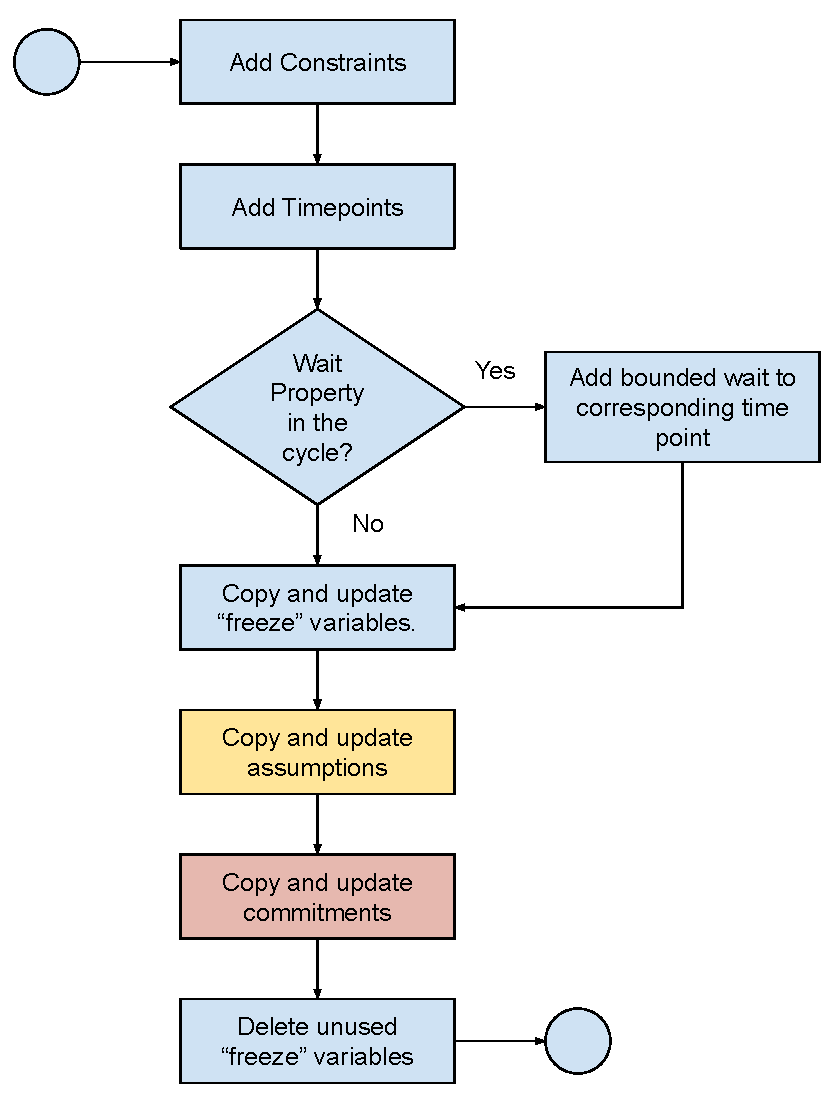
\includegraphics[width=0.7\textwidth]{images/algorithm.pdf}
	\caption{Flowchart for the merging algorithm that combines a sequence of micro properties of a cyclic sub-graph of the PPA into a Pipeline Property.}
	\label{fig:algorithm-flow}
\end{figure}

The first step of the merging algorithm is \textbf{Add Constraints}. As shown in the micro properties of Fig.~\ref{fig:add-ex-wb-micro-ppt}, \textit{DeSCAM} generates the properties already including one constraint, \textit{no\_reset}. This constraint informs the \textit{property checking tool} that, for the duration of the operation, there should be no \textit{reset} signal. At this step, the designer must include any other constraints that are valid for the entire duration of the operation. One example is a constraint that specify the memory protocol, so the tool knows how the memory \textit{input} signals behave.

For the \textbf{Add Timepoints} step, one timepoint variable is created referring to the commitments of each micro property. The micro properties include the $t\_end$ timepoint variable, see line 4 of Fig.~\ref{subfig:add-if-micro-ppt}, and these timepoints are integrated to the resulting pipeline property, e.g. $t\_id$, $t\_ex$, and $t\_wb$ representing the time for each pipeline stage.

Next, the cyclic path is analysed in order to identify if there are \textit{wait} operations present. If that is the case, the step \textbf{Add bounded wait to corresponding timepoint} is executed, where each \textit{wait} operation must be converted into a \textit{bounded wait} to the corresponding \textit{input} signal and included for the right timepoint. The micro properties in Fig.~\ref{fig:load-mem-wait-micro-ppt} show the transitions for a \textit{LOAD} instruction at the \textit{MEM} stage. In (a) the IUV is at stage \textit{MEM} and the \textit{sync} signal from the memory arrives. Then, the \textit{LOAD} instruction moves forward to the \textit{WB} stage. In (b), the wait operation proves that the IUV remains at the \textit{MEM} stage until the \textit{sync} signal comes. In this case, a \textit{bounded wait} for the \textit{input} signal \textit{data\_req\_out\_sync} is created at $t\_wb$, i.e. the timepoint corresponding to the write back stage.

\begin{figure}[htb!]
     \centering
     \begin{subfigure}[b]{\textwidth}
         \begin{lstlisting}
    property PDD_LOAD_MEM;
    dependencies: no_reset;
    for timepoints:
        t_end = t+1;
    freeze:
        PC_at_t = PC@t,
        fetched_instr_at_t = fetched_instr@t,
        data_in_sig_at_t = data_in_sig@t;
    assume:
        at t: MEM;
        at t: data_req_out_sync;
    prove:
        at t_end: WB;
        at t_end: PC == PC_at_t;
        at t_end: fetched_instr == fetched_instr_at_t;
        at t_end: wb_regWrEn = ex_regWrEn;
        at t_end: wb_regAddr = ex_regAddr;
        at t_end: wb_regData = data_in_sig_at_t;
        during [t+1, t_end]: instr_req_out_notify == false;
        during [t+1, t_end]: data_req_out_notify == false;
    end property;\end{lstlisting}
         \caption{Micro property describing operation from \textit{MEM} stage to \textit{WB} stage when the \textit{sync} signal from data memory arrives.}
         \label{subfig:load-mem-micro-ppt}
     \end{subfigure}
     \hfill
     \begin{subfigure}[b]{\textwidth}
         \begin{lstlisting}
    property PDD_LOAD_WAIT_MEM;
    dependencies: no_reset;
    for timepoints:
        t_end = t+1;
    freeze:
        PC_at_t = PC@t,
        fetched_instr_at_t = fetched_instr@t;
    assume:
        at t: MEM;
        at t: !data_req_out_sync;
    prove:
        at t+1: MEM;
        at t+1: PC == PC_at_t;
        at t+1: fetched_instr == fetched_instr_at_t;
        at t+1: instr_req_out_notify == false;
        at t+1: data_req_out_notify == false;
    end property;\end{lstlisting}
         \caption{Micro property describing the \textit{wait} operation when the IUV is in the \textit{MEM} stage waiting for the synchronization signal from the data memory}
         \label{subfig:load-wait-micro-ppt}
     \end{subfigure}
        \caption{Example of micro properties generated for an \textit{LOAD} instruction from an enhanced SystemC-PPA processor description with states inserted to each pipeline stage. The property in (a) refers to the transition between \textit{MEM} and \textit{WB} stages, and the property in (b) shows the \textit{wait} operation.}
        \label{fig:load-mem-wait-micro-ppt}
\end{figure}

In the \textbf{Copy and update “freeze” variables} step, the variables present at the “\textit{freeze}” section of each micro property, e.g. line 6 of Fig.~\ref{subfig:add-if-micro-ppt}, are copied into the merged property. The names of the variables are updated to match the created timepoint for the corresponding micro operation.

The steps marked in yellow and red refer to merging assumptions and commitments. They are broken down into further steps and are presented in figures \ref{fig:algorithm-assumptions-flow} and \ref{fig:algorithm-commitments-flow}. The last step is to \textbf{Delete unused “freeze” variables}, where the variables that are no longer used at the assumptions and commitments are excluded. 

\begin{figure}[htb!]
	\centering
	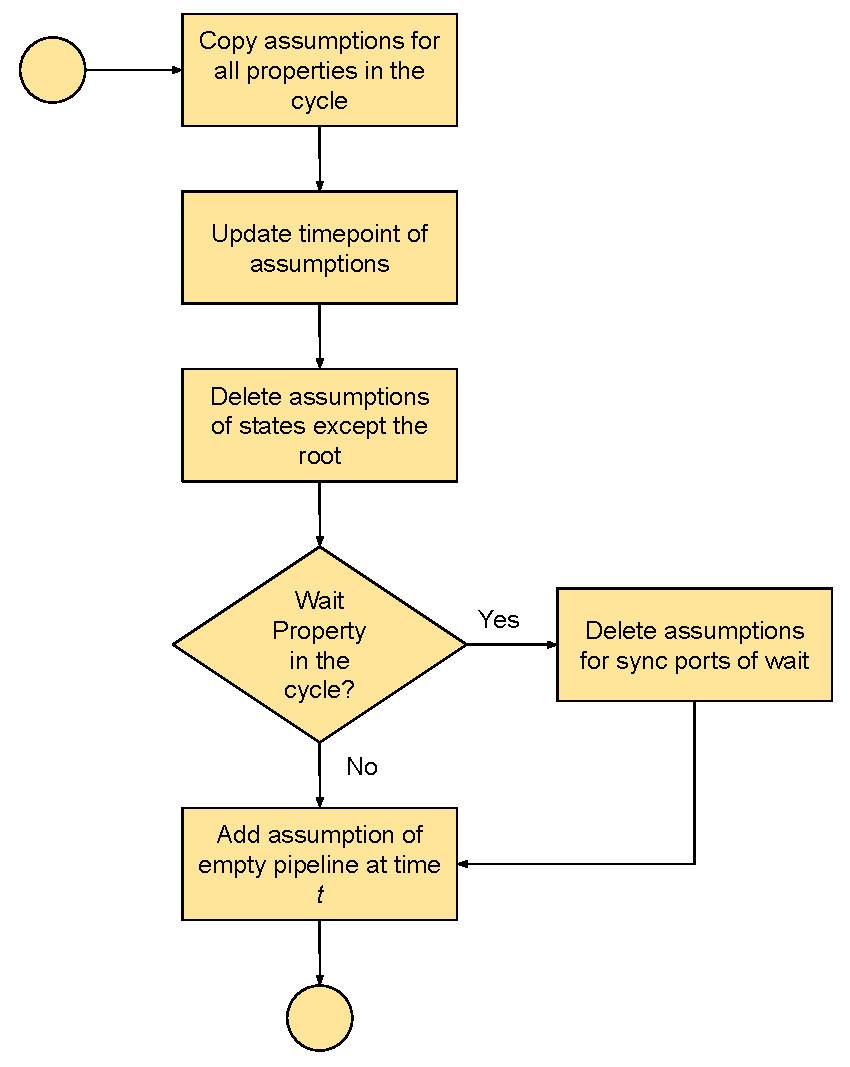
\includegraphics[width=0.7\textwidth]{images/algorithm_assumptions.pdf}
	\caption{Flowchart for merging assumptions from micro properties into assumptions of the pipeline property.}
	\label{fig:algorithm-assumptions-flow}
\end{figure}

The first step towards merging the assumptions, as shown in Fig.~\ref{fig:algorithm-assumptions-flow} is to \textbf{Copy assumptions} for all micro properties in the cycle into the assumptions field of the pipeline property. Then, \textbf{Update timepoint of assumptions} according to the timepoint created for the corresponding micro property. Next,\textbf{ Delete assumptions of states except the root} state. The resulting pipeline property will have its starting state at time $t$ being the \textit{root} state, e.g. the \textit{IF} state. The designer must refine this state to represent the \textit{ready to fetch} state reached after \textit{reset}.

If there is a \textit{wait} operation in the cycle, the next step is to \textbf{Delete assumptions for sync ports of wait} properties. This is necessary because the synchronization signal is already included at the \textit{bounded wait}.

The final step to complete the assumption part of the pipeline property is to \textbf{Add assumption of empty pipeline at time $t$}. This assumption is not generated by \textit{DeSCAM} and must be refined by the designer. It constrains the IUV to execute in an empty pipeline.

\begin{figure}[htb!]
	\centering
	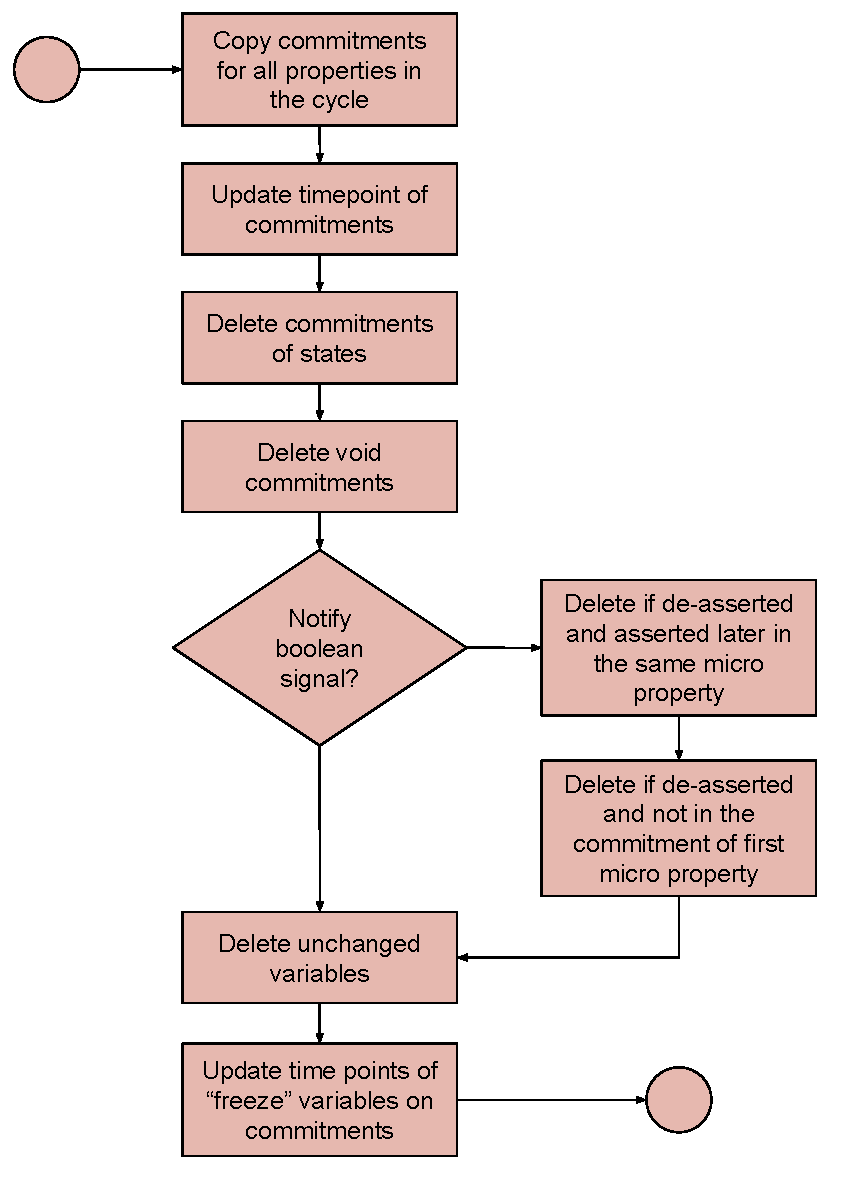
\includegraphics[width=0.7\textwidth]{images/algorithm_commitments.pdf}
	\caption{Flowchart for merging commitments from micro properties into commitments of the pipeline property.}
	\label{fig:algorithm-commitments-flow}
\end{figure}

Similarly to the assumptions, the commitment steps start with \textbf{Copy commitments for all properties in the cycle}, \textbf{Update timepoint of commitments}, and then \textbf{Delete commitments of states}. The next step it to \textbf{Delete void commitments}, e.g. the commitment in line 14 of Fig.~\ref{subfig:add-id-micro-ppt}. This commitment selects a time interval between $t+1$ and $t\_end-1$, which is void. In practice, this commitment can be kept in the property as it will not interfere in the property checking. However, removing it increases the readability of the resulting property.

The next two steps are related to \textit{notify} signals derived from communication ports of the ESL model. The \textbf{Delete if de-asserted and asserted later in the same micro property} step is intended to delete the commitments where the \textit{notify} signals are de-asserted for a time interval and then asserted later in the same micro property. This is a consequence of the pipeline behaviour where the time of interest for the commitments of each micro operation is the timepoint of the current pipeline stage.

The \textbf{Delete if de-asserted and not in the commitment of first micro property} step refers to the refinement of the commitments that are not from the micro property starting from the \textit{root} state. The \textit{notify} signal is only kept if it is asserted, otherwise it is not important for that pipeline stage. Keeping such commitment would create contradicted commitments. This does not apply to the commitments from the first micro operation because any \textit{output} signal is determined at this time as a result of the empty pipeline assumption. The commitments in lines 18 and 19 of the property in Fig.~\ref{subfig:add-id-micro-ppt} are examples of commitments that are deleted by the merging algorithm.

The next step, \textbf{Delete unchanged variables}, follows the same idea and deletes the variables which values are assigned to the same previous value, e.g. commitments of lines 13 and 14 of Fig.~\ref{subfig:add-id-micro-ppt}.

\textbf{Update time points of “\textit{freeze}” variables on commitments} is the final step for refining the commitments. It changes the names of the “\textit{freeze}” variables according to the corresponding timepoint tag assigned to the referred micro property. E.g. the micro property in Fig.~\ref{subfig:add-id-micro-ppt} used the variable \textit{PC\_at\_t} in the commitment of line 13. Since the timepoint $t$ becomes $t\_id$ with the merging step, by this rule the variable would become $PC\_at\_t\_id$. 

One special case for this step refers to the signals derived from the data port of \textit{blocking} interfaces. Consider the commitment in line 18 of the property in Fig.~\ref{subfig:load-mem-micro-ppt}. The signal \textit{data\_in\_sig} corresponds to the message signal of the data memory \textit{blocking} port. This variable relates to the data that arrives with the \textit{sync} signal \textit{data\_req\_out\_sync} in the \textit{wait} operation. In this case, the variable in line 18 must be updated to the timepoint when the data comes after the wait, i.e. the timepoint with the \textit{bounded wait}, $t\_wb$.

The listing in Fig.~\ref{fig:add-ptt-merg-algorithm} shows a property resulting form the merging algorithm applied to the four micro properties, shown in Fig.~\ref{fig:add-if-id-micro-ppt} and Fig.~\ref{fig:add-ex-wb-micro-ppt}, generated for an \textit{ADD} instruction.

\begin{figure}[htb!]
    \begin{lstlisting}
    property PIPE_PDD_ADD;
    dependencies: 
        no_reset,
        instr_mem;
    for timepoints:
        t_id = t+1,
        t_ex = t_id+1,
        t_wb = t_ex+1,
        t_end = t_wb+1;
    freeze:
        PC_at_t = PC@t;
    assume:
        at t: IF;
        at t: empty_pipeline;
        at t_id: getInstrType(fetched_instr) == ADD;
    prove:
        at t_id: PC == PC_at_t + 4;
        at t_id: fetched_instr == instr_in_sig;
        at t_id: operands == getOperandsFromRegFile(fetched_instr);
        at t_id: instr_req_out_notify == true;
        during [t+1, t_id]: data_req_out_notify == false;
    
        at t_ex: ex_regData == operands.rs1 + operands.rs2;
        at t_ex: ex_regAddr == operands.rd;
        at t_ex: ex_regWrEn == true;
        during [t_id+1, t_ex]: data_req_out_notify == false;
    
        at t_wb: wb_regWrEn = ex_regWrEn;
        at t_wb: wb_regAddr = ex_regAddr;
        at t_wb: wb_regData = ex_regData;
        during [t_ex+1, t_wb]: data_req_out_notify == false;
    
        at t_end: RegFile[wb_regAddr] == (wb_regWrEn) ? wb_regData : RegFile[wb_regAddr];
        during [t_wb+1, t_end]: data_req_out_notify == false;
    end property;\end{lstlisting}
    \caption{Pipeline Property for an ADD instruction. This property is the result of the pipeline algorithm applied to the micro properties in Fig.~\ref{fig:add-if-id-micro-ppt} and Fig.~\ref{fig:add-ex-wb-micro-ppt}.}
    \label{fig:add-ptt-merg-algorithm}
\end{figure}

A constraint for the instruction memory protocol is added at the \textit{dependencies} part (line 4). One timepoint relating to the commitments of each micro properties is added to the \textit{timepoints} part (lines from 6 to 9). The assumptions include the \textit{IF} state that must be refined into the \textit{ready to fetch} state, the \textit{empty\_pipeline} constraint, and the triggering condition at $t\_id$. This assumption determines the type of instruction, and it comes from the \textit{ID} micro property (Fig.~\ref{subfig:add-id-micro-ppt}). The commitments comprise four sets of commitments imported from each micro operation; the \textit{IF} operation from line 17 to 21, the \textit{ID} operation from line 23 to 26, the \textit{EX} operation from line 28 to 31, and the \textit{WB} operation in lines 33 and 34.

The listing in Fig.~\ref{fig:load-ptt-merg-algorithm} shows the timepoint part of a pipeline property for the \textit{LOAD} instruction. Line 6 shows the timepoint derived from the \textit{wait} property where the \textit{bounded wait} upon the \textit{sync} signal is included. 

\begin{figure}[htb!]
    \begin{lstlisting}
    property PIPE_PDD_LOAD;
    [...]
    for timepoints:
        t_id = t+1,
        t_mem = t_id+1,
        t_wb = t_mem+1..max_wait_dmem waits_for (data_req_out_sync),
        t_end = t_wb+1;
    [...]
    end property;\end{lstlisting}
    \caption{Timepoint of a Pipeline Property for an \textit{LOAD} instruction.}
    \label{fig:load-ptt-merg-algorithm}
\end{figure}

After running the Pipeline Algorithm, a set of constrained pipeline properties is obtained. In order to have a complete set of properties, a set of \SSQED{} properties must be created as presented in Sec.~\ref{section:s2qed}. In order to further support the designer, a plugin for \textit{DeSCAM} was implemented to create the setup environment to check the \SSQED{} property set. This implementation is presented in Sec.~\ref{section:plugio-s2qed-top}.

The extended PDD method for pipelined processors guides the hardware designer through simple steps when refining the generated property set. Nonetheless, it still constitutes more effort when compared to the original PDD method for non-pipelined designs. However, the majority of the steps composing the proposed algorithm can be automated and included as an extension for the \textit{DeSCAM} tool. Future work will include both constrained pipeline properties set and \SSQED{} properties set as an extension to \textit{DeSCAM}.

\section{The Plugin for a \SSQED{} Template}
\label{section:plugio-s2qed-top}

Sec.~\ref{section:s2qed} presents how the \SSQED{} approach can be employed to prove the case-split test and achieve completeness. In order to apply this approach, a special setup with two \textit{identical} and \textit{independent} instances of the DUV is required. A plugin for \textit{DeSCAM} was implemented in this work in order to assist the hardware designer to create such setup. A schematic diagram of a configuration for allowing property check with the \SSQED{} approach is shown in Fig.~\ref{fig:s2qed-top-diagram}. 

\begin{figure}[htb!]
	\centering
	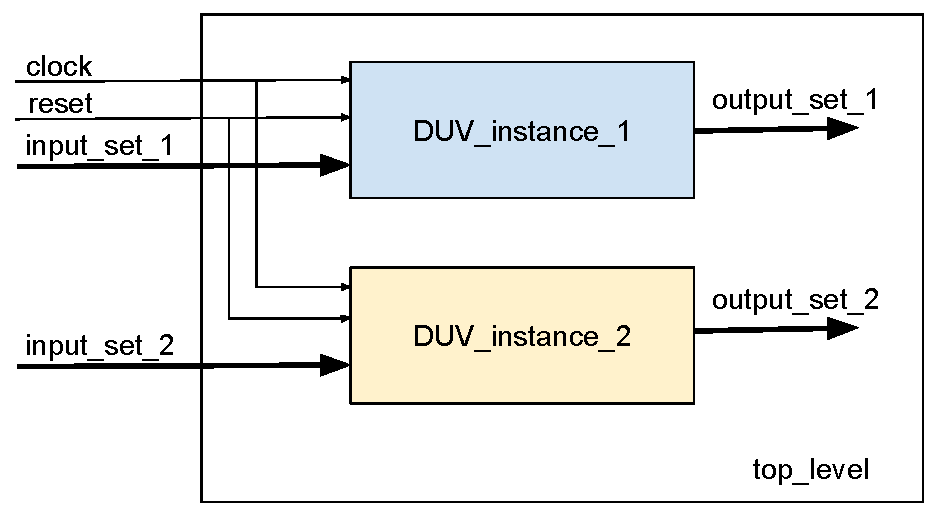
\includegraphics[width=0.7\textwidth]{images/top_s2qed.pdf}
	\caption{Diagram of a setup for proving the \SSQED{} model.}
	\label{fig:s2qed-top-diagram}
\end{figure}

The plugin can be optionally used by the designer to generated a HDL template for the configuration shown in Fig.~\ref{fig:s2qed-top-diagram}. The top-level generated has, besides the \textit{clock} and \textit{reset} signals, a duplicate set of \textit{inputs} matching the \textit{inputs} of the two DUV instances. The naming for \textit{inputs}, \textit{outputs} and signals corresponds to the names in the HDL template generated for the DUV by \textit{DeSCAM}. During the \textit{refine-and-implement} process, the designer must update the top-level according to the changes made to the \textit{I/O ports} in the DUV. If the designer does not use the HDL template for the DUV, the structure of the top-level template for the \SSQED{} configuration can still be used. However, the \textit{I/O ports} and signals must be modified accordingly.

The listing in Fig.~\ref{fig:s2qed-top-example} shows an example of a HDL verification top-level generated for a DUV that has one \textit{input} vector of 32 bits and an \textit{output} signal. The ports of \textit{myDUV\_top} include \textit{input} signals for the two instances (lines 6 and 7). Port signals are created from line 10 to 14 for connecting the \textit{I/O} of both instances. The \textit{inputs} are assigned to their corresponding signals in lines 17 and 19.  Finally, the two DUV’s are instantiated from lines 21 to 33.

\begin{figure}[htb!]
    \begin{lstlisting}[language=c++]
    import top_level_types::*;
    import myduv_types::*;
    module myDUV_top (
        input logic clk,
        input logic rst,
        input bit[31:0] d_in_i1,
        input bit[31:0] d_in_i2
    );
    // Port signals for instance 1
    bit[31:0] d_in_s1;
    logic d_out_s1;
    // Port signals for instance 2
    bit[31:0] d_in_s2;
    logic d_out_s2;
    // Input signals assignments
    // Assignment fot instance_1
    assign d_in_s1 = d_in_i1;
    // Assignment fot instance_2
    assign d_in_s2 = d_in_i2;
    // Instance 1
    myDUV myDUV_inst_1 (
        .clk ( clk ),
        .rst ( rst ),
        .d_in ( d_in_s1 ),
        .d_out ( d_out_s1 )
    );
    // Instance 2
    myDUV myDUV_inst_2 (
        .clk ( clk ),
        .rst ( rst ),
        .d_in ( d_in_s2 ),
        .d_out ( d_out_s2 )
    );
    endmodule\end{lstlisting}
    \caption{Timepoint of a Pipeline Property for an \textit{LOAD} instruction.}
    \label{fig:s2qed-top-example}
\end{figure}


\newpage
% ----------------------------------------------------------
% The RI5cy Study Case
% ----------------------------------------------------------
\chapter{The RI5CY Case Study}
\label{chapter:ri5cy}

The algorithm to generate Pipeline Properties, proposed in Chap.~\ref{chapter:algorithm},  was evaluated with a case study for the RI5CY processor core. RI5CY is a 4-stage pipeline processor core based on the RISC-V architecture. Its implementation is open-source and powered by PULP Platform \cite{pulp}, and it is now part of  the OpenHW Group\cite{openhw}.

For this case study, a \textit{SystemC-PPA-compliant} \cite{paper-pdd} model for the chosen core was implemented as a sequential CPU model. The properties were then automatically generated using DeSCAM \cite{descam}. From these automatically generated properties, the Pipeline Properties were finally created using the merging Pipeline Algorithm. 

This chapter starts with a brief discussion about the RISC-V Implementation Set Architecture and the RI5CY processor core in Sec.~\ref{section:ri5cy_core}. Next, the ESL implementation compliant to the SystemC-PPA specification is detailed in Sec.~\ref{section:ri5cy-systemc-ppa}. Then, the DeSCAM generated properties and the Pipeline Properties are presented and explained in Sec.~\ref{section:ri5cy_pipe_ppt}. Finally the \SSQED{} Properties are presented in Sec.~\ref{section:ri5cy-s2qed-ppt}.

\section{The RI5CY Processor Core}
\label{section:ri5cy_core}

\textit{Instruction Set Architecture}~(ISA), is the set of instructions that a computer, or more specifically a processor core, can execute. Some of the specification provided by the ISA are which operations the processor can perform, how the memory is addressed and the type and size of the instruction operands \cite{book-comp-arch}.

A \textit{Reduced Instruction Set Computer}~(RISC) is a computer that has a small set of instructions. These instructions have a simple fixed length encoding, and they take similar number of \textit{clock} cycles to execute \cite{book-comp-arch}. Some examples of RISC architectures are AMRv7, MIPS and RISC-V.

RISC-V is an open ISA that offers both a small base integer ISA that can be used by itself, and optional standard extensions. As an open and free to use architecture, it was initially intended to support computer architecture research and education \cite{spec-riscv}. Even so, its popularity increased rapidly and there are open-source simulators, compilers, debuggers and implementations in HDL for RISC-V available \cite{book-comp-org}. One of these open-source implementations is the RI5CY processor powered by PULP Platform \cite{pulp}. This implementation is used as case study in the present work and some important details are presented in this section. 

RI5CY is an in-order \textit{32 bits} core and has a pipeline with 4 stages. Besides the support for the \textit{RV32I} Base Integer Instruction Set, it has also support for the \textit{RV32C} Standard Extension for Compressed Instructions and \textit{RV32M} Integer Multiplication and Division Instruction Set Extension, and optional support for \textit{RV32F} Single Precision Floating Point Extensions. This core also implements the following PUPL specific extensions:  Post-Incrementing load and stores, Multiply-Accumulate extensions, ALU extensions, and Hardware Loops.

However, this case study is focused on the \textit{32bits} Integer Base Instructions set as detailed in Sec.~\ref{section:ri5cy-systemc-ppa} of this chapter. Before that, however, some aspects of the pipeline, memory protocol and Load-Store Unit of the RI5CY core are briefely discussed. These implementation aspects are important for the understanding of the ESL model and for the property generation as well.

For detailed information about all the RI5CY extensions, the reader may refer to the RI5CY User Manual \cite{manual-ri5cy}.

\subsection*{RI5CY Pipeline}

The RI5CY core implements a 4-stage pipeline: instruction fetch (\textit{IF}), instruction decode (\textit{ID}), execute (\textit{EX}) and write-back (\textit{WB}). However, most of the instructions in the base integer set, like arithmetic and logic operations, uses only the first three stages. The \textit{WB} stage is used, for example, when loading data from the data memory. Fig.~\ref{fig:ri5cy_pipeline} depicts the pipeline structure and its main signals.

\begin{figure}[htb!]
	\centering
	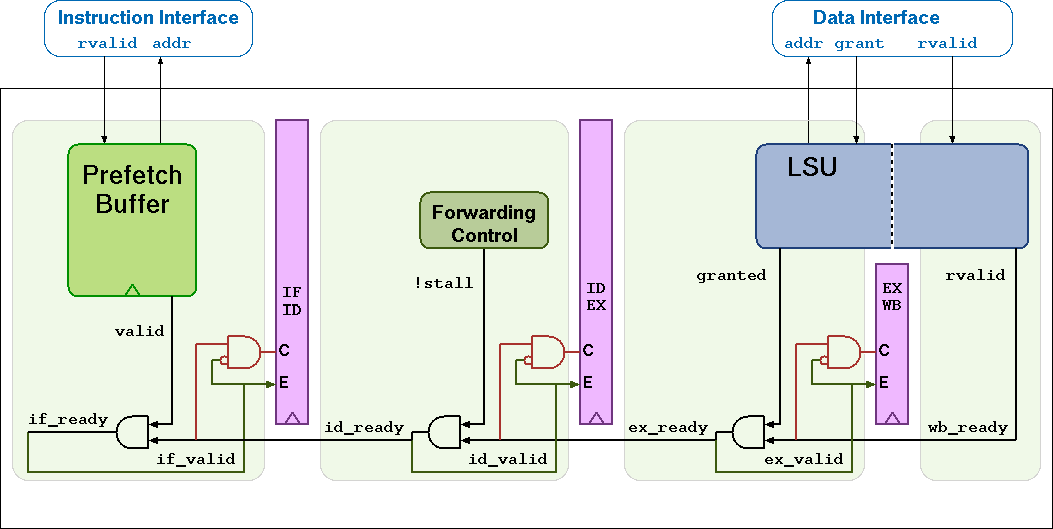
\includegraphics[width=\textwidth]{images/ri5cy_pipeline.png}
	\caption{RI5CY pipeline diagram \cite{manual-ri5cy}.}
	\label{fig:ri5cy_pipeline}
\end{figure}

The \textit{ready} signal of each stage propagates from right to left and are used to inform the previous stage that the current stage is ready to operate. In this sense, each stage can finish its execution independently from the previous, but they cannot propagate if the next one is not ready, the pipeline \textit{stalls}. 

\subsection*{RI5CY Load-Store Unit}

\textit{The Load-Store Unit}~(LSU) is the component of the core responsible to access the data memory. As shown in Fig.~\ref{fig:ri5cy_pipeline}, the LSU belongs to two pipeline stages: \textit{EX} and \textit{WB}. It means that a request to the data memory is sent already in the \textit{EX} stage. To illustrate this behaviour better, consider a \textit{LOAD} instruction in the \textit{ID} stage. In the next \textit{clock} cycle, the access address is computed in the \textit{EX} stage, and the LSU sends a request to the data memory in the same cycle. When the data arrives from memory, the LSU will write it to the correspondent register in the \textit{WB} stage. The memory access protocol is detailed next.

\subsection*{RI5CY Memory Access Protocol}

In order to access the data memory, the LSU sets the output address with the right address and sends a request signal. The LSU waits for a grant signal from the memory that can come in the same \textit{clock} cycle as the request or any number of \textit{clock} cycles later. After receiving the grant signal, the LSU can optionally change the outputs and make a new request or just set the request signal to \textit{low}. If it was a read from memory request, e.g. \textit{LOAD} instruction, the memory will send the data along with a valid signal one or more \textit{clock} cycles after the grant signal. All the LSU signals can be found in Table~\ref{tab:lsu-signals} with a brief description. 

\begin{table*}[htb!] 
	\centering 
	\caption{LSU port signals of RI5CY processor\cite{manual-ri5cy}.} 
	\label{tab:lsu-signals}
	\begin{tabular}{l|c|p{7cm}} 
		\multicolumn{1}{c}{\bfseries Signal} & \multicolumn{1}{c}{\bfseries Port Direction} & \multicolumn{1}{c}{\bfseries Description} \\     
		\hline	
		$data\_req\_o$  &  output & Request ready, must stay high until $data\_gnt\_i$ is        high for one cycle \\
		\hline
		$data\_addr\_o$[31:0]  &  output & Address \\
		\hline
		$data\_we\_o$  &  output & Write Enable, high for writes, low for reads. Sent            together with $data\_req\_o$ \\
		\hline
		$data\_wdata\_o$[31:0]  &  output & Data to be written to memory, sent together with     $data\_req\_o$ \\
		\hline
		$data\_rdata\_i$[31:0]  &  input & Data read from memory \\
		\hline
		$data\_rvalid\_i$  &  input & $data\_rdata\_i$ holds valid data when                     $data\_rvalid\_i$ is high. This signal will be high for exactly one cycle per        request. \\
		\hline
		$data\_gnt\_i$  &  input & The other side accepted the request. $data\_addr\_o$ may     change in the next cycle \\
		\hline
	\end{tabular} 
\end{table*}

The instruction memory access performed by the instruction fetcher of the core is similar to the data memory protocol. The only difference is that the instruction fetcher does not have any \textit{write} interface, since the instruction memory is only read by the core. The instruction fetcher signals are presented in Table~\ref{tab:imem-signals}.

\begin{table*}[htb!] 
	\centering 
	\caption{Instruction memory port signals of RI5CY processor \cite{manual-ri5cy}.} 
	\label{tab:imem-signals}
	\begin{tabular}{l|c|p{7cm}} 
		\multicolumn{1}{c}{\bfseries Signal} & \multicolumn{1}{c}{\bfseries Port Direction} & \multicolumn{1}{c}{\bfseries Description} \\     
		\hline	
		$instr\_req\_o$  &  output & Request ready, must stay high until $instr\_gnt\_i$ is high for one cycle \\
		\hline
		$instr\_addr\_o$[31:0]  &  output & Address \\
		\hline
		$instr\_rdata\_i$[31:0]  &  input & Data read from memory \\
		\hline
		$instr\_rvalid\_i$  &  input & $instr\_rdata\_i$ holds valid data when $instr\_rvalid\_i$ is high. This signal will be high for exactly one cycle per request. \\
		\hline
		$instr\_gnt\_i$  &  input & The other side accepted the request. $instr\_addr\_o$ may change in the next cycle \\
		\hline
	\end{tabular} 
\end{table*}

\section{SystemC-PPA Implementation}
\label{section:ri5cy-systemc-ppa}

For this case study, an ESL model was implemented to comply with the RI5CY core implementation. The core user manual along with the existent RTL implementation were used to extract the specifications for the system-level. Therefore, the PDD flow is not followed to implement the RTL design, as it already exists. The goal was to create a SystemC-PPA compliant model of a processor based on the RISC-V architecture such that the generated set of properties would hold to its RTL implementation.

The proposed ESL model does not comprise the RI5CY extensions and implements only a restrict set of instructions from the \textit{RV32I} Base Integer Instruction set of the RISC-V ISA. They are the arithmetic and logic instructions, \textit{load} and \textit{store} instructions, \textit{branch} and \textit{jump} instructions, and \textit{LUI} and \textit{AUIPC}.

The block diagram in Fig.~\ref{fig:sim-ri5cy-diagram} shows the configuration implemented for simulating the ESL model of the core. The Register File and the Memory modules were imported from the RISC-V example in the DeSCAM repository \cite{descam}. The Register File has 32 registers where register 0 is \textit{read-only}, and the Memory module implements a memory for both instruction and data. For this reason, a memory interface had to be implemented in order to parse memory requests from the core, as it has separate ports for instructions and data.

\begin{figure}[htb!]
	\centering
	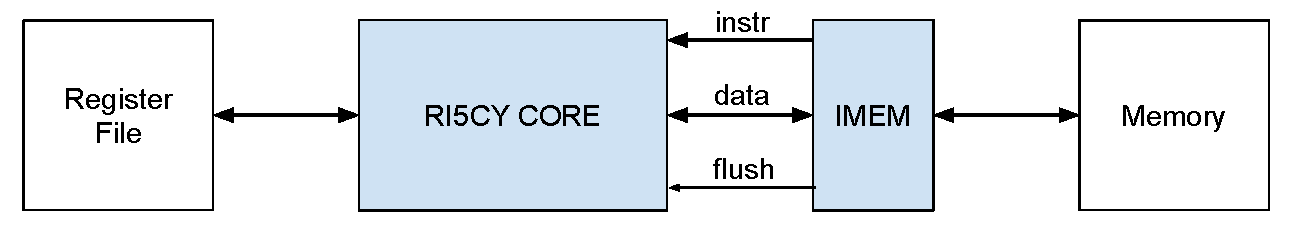
\includegraphics[width=\textwidth]{images/sim-block-diagram.pdf}
	\caption{Block diagram of the system-level implemented for the RI5CY core.}
	\label{fig:sim-ri5cy-diagram}
\end{figure}

As shown in the block diagram of Fig.~\ref{fig:sim-ri5cy-diagram}, the RI5CY CORE has four \textit{I/O} interfaces. Two for memory transactions, instruction and data, one for communicating with the Register File and a \textit{flush input} signal. Their declaration can be seen in the code snippet in Fig.~\ref{fig:ri5cy-sc-module} that shows the class declaration of the SystemC module of the processor core.

\begin{figure}[htb!]
    \begin{lstlisting}[language=c++]
    class ISA_ri5cy : public sc_module {
    public:
        //Constructor
        SC_HAS_PROCESS(ISA_ri5cy);
        ISA_ri5cy(sc_module_name name) {
        SC_TH   READ(run);
        }
        //ports for communication with instr mem
        master_in<unsigned int> instr_in;
        master_out<unsigned int> instr_req;
        
        //ports for communication with data mem
        master_in<unsigned int> data_in;
        blocking_out<CUtoME_IF> data_out;
        
        // ports for communication with register file
        shared_in<RegfileType> fromRegsPort;
        master_out<RegfileWriteType> toRegsPort;
        
        // flushing signal for RTL (always false for ESL simulation)
        shared_in<bool> flush_in;
        
        enum Sections {FETCH_PH, DECODE_PH, EXECUTE_PH};
        // [...] variables and helping functions
        void run(); // fsm
    };\end{lstlisting}
    \caption{SystemC class of the RI5CY core.}
    \label{fig:ri5cy-sc-module}
\end{figure}

The instruction memory interface is of type \textit{Master}, and it has two signals. One \textit{output} signal to send the request address, and an \textit{input} signal that receives the requested instruction. The \textit{Master} interface is \textit{non-blocking} and simplifies the instruction memory protocol. Therefore, no wait signal is created for this interface. This is possible because each property will have a triggering condition that an instruction of a specific type is fetched. Thus, no waiting upon the instruction memory is needed.

On the other hand, the data memory interface has a \textit{blocking output} port for making the requests, and a \textit{Master input} port to read the data. This means that the processor must wait for a synchronization signal from the data memory upon a request. If the request is a \textit{read} operation, the incoming data is available after synchronization. For this reason, the \textit{input} port is \textit{non-blocking} of type \textit{Master}.

The interface for communicating with the Register file is also \textit{non-blocking}. In fact, the register file is modeled as an external module at the system-level, however it is embedded to the core in the RTL implementation. This modeling decision illustrates that the RTL implementation choices are not constrained by the system-level model. In this case, during the \textit{refine-and-implement} phase of the PDD flow, the designer would have simply to match the ESL ports to the internal signals of the RTL. Since the register can be read as an internal variable, the type of interface employed was the \textit{Shared} interface for \textit{input} and \textit{Master} for \textit{output}, both are \textit{non-blocking} interfaces.

The \textit{flush} signal is part of the enriched SystemC-PPA, and it is included in the model to reflect the flushing behaviour of the pipeline. Execution of some instructions may cause the pipeline to flush, e.g. when a branch instruction is evaluated and the branch is taken, the consecutive instruction, already fetched and executing in the pipeline, must be flushed. This behaviour is not modeled by the ESL because its execution is sequential, and an instruction only starts executing after the previous one is concluded. Therefore, there is no need for \textit{flushing}. The inclusion of the \textit{flush} signal at the ESL should not change its behaviour during simulation, but it will change the generated property set. The properties will have one operation for when the \textit{flush} signal is asserted and one for when it is not. The designer will then refine the flush macro into the corresponding implemented signal, e.g. the branch decision signal. 

The IMEM module is a memory interface that parses the separated instruction and data memory requests into a request to the single port of the memory model. It also feeds the core with a \textit{flush} signal always set to false, so it does not interfere in the simulation. This module, like the Register File and the Memory model, is only used for simulating the RI5CY core. The only module that is interpreted by DeSCAM to generate the property set is the core module, which is the DUV.

An outline of the \textit{run()} function is shown in Fig.~\ref{fig:ri5cy-run-outline}. This function implements the main behaviour of the core. It runs infinitely and is divided into three sections, \textit{FETCH\_PH}, \textit{DECODE\_PH} and \textit{EXECUTE\_PH}. These three phases directly relate to the pipeline stages of the processor. However, the write back stage is not explicitly shown. This is because this \textit{WB} stage is only used by the LSU, and its important state is created as a result of the memory \textit{blocking} interface. 

\begin{figure}[htb!]
    \begin{lstlisting}[language=c++]
    void ISA_ri5cy::run() {
        nextsection = Sections::FETCH_PH;
        while (true){
            if (section == Sections::FETCH_PH){
            //[...]
            nextsection = Sections::DECODE_PH;
            } else if (section == Sections::DECODE_PH){
            //[...]
            nextsection = Sections::EXECUTE_PH;
            } else if (section == Sections::EXECUTE_PH) {
                if(getInstrType(encodedInstr) != InstrType::INSTR_UNKNOWN){
                    if (getEncType(encodedInstr) == ENC_R){...}
                    else if (getEncType(encodedInstr) == ENC_I_I){...}
                    else if (getEncType(encodedInstr) == ENC_I_L) {...}
                    else if (getEncType(encodedInstr) == ENC_S) {...} 
                    else if (getEncType(encodedInstr) == ENC_B) {...} 
                    else if (getEncType(encodedInstr) == ENC_U) {...} 
                    else if (getEncType(encodedInstr) == ENC_J) {...} 
                    else if (getEncType(encodedInstr) == ENC_I_J) {...}
            }
            nextsection = Sections::FETCH_PH;
    }}}\end{lstlisting}
    \caption{Code outline from the \textit{run()} function of RI5CY core.}
    \label{fig:ri5cy-run-outline}
\end{figure}

\subsection*{The FETCH\_PH section}

This section is depicted in Fig.~\ref{fig:ri5cy-fetch-ph} and it simply fetches a new instruction. The variable \textit{fromReset} is only asserted in the first time this loop is executed. It is used to implement the \textit{reset} behaviour where the first request to the instruction memory is done. For the remaining execution, the instruction requests are done at the decode phase.

\begin{figure}[htb!]
    \begin{lstlisting}[language=c++]
    if (section == Sections::FETCH_PH){
        if(fromReset){
            instr_req->master_write(iaddr);
            pcIf = 0;
        }
        insert_state("IF");
        instr_in->master_read(encodedInstr);
        nextsection = Sections::DECODE_PH;
    }\end{lstlisting}
    \caption{FETCH\_PH section from the \textit{run()} function of RI5CY core.}
    \label{fig:ri5cy-fetch-ph}
\end{figure}

\subsection*{The DECODE\_PH section}

This section is shown in the code snippet of Fig.~\ref{fig:ri5cy-decode-ph}. The main attributions of this phase are updating the instruction fetching address, sending a new request to the instruction memory, and reading the register file. 

\begin{figure}[htb!]
    \begin{lstlisting}[language=c++]
    else if (section == Sections::DECODE_PH){
        flush_in->get(flush);
        if (flush) {
            iaddr = pcIf - 4 + getImmediate(prevInstr);
            instr_req->master_write(iaddr);
            prevInstr = encodedInstr;
            nextsection = Sections::FETCH_PH;
        } else {
            if(getEncType(encodedInstr) == ENC_J) {
            iaddr = pcIf + getImmediate(encodedInstr);
            instr_req->master_write(iaddr);
            insert_state("ID_J");
        } else if (getEncType(encodedInstr) == ENC_I_J) {
            fromRegsPort->get(regfile); //Read register contents
            iaddr = readRegfile(getRs1Addr(encodedInstr), regfile) + getImmediate(encodedInstr);
            iaddr = iaddr & 0xFFFFFFFE;
            instr_req->master_write(iaddr);
            insert_state("ID_I_J");
        } else {
            iaddr = iaddr + 4;
            instr_req->master_write(iaddr);
            insert_state("ID");
        }
        fromRegsPort->get(regfile); //Read register contents
        nextsection = Sections::EXECUTE_PH;
    }}\end{lstlisting}
    \caption{DECODE\_PH section from the \textit{run()} function of RI5CY core.}
    \label{fig:ri5cy-decode-ph}
\end{figure}

For the RI5CY core, the fetching address is not normally computed based on the PC, it is computed by incrementing the previous fetched address. The PC is used for instructions such as \textit{branch} and \textit{jumps} that need the address of the current executing instruction. The \textit{jump} instructions are executed already at the decode phase. Then, if the fetched instruction is a \textit{jump}, the new instruction address computation and the request to this address are done already in this section. The type \textit{ENC\_J} represents the instruction \textit{jal}, where the jumping address, i.e. the address of the next instruction to be fetched, is computed by adding the PC to the immediate field. The \textit{ENC\_I\_J} corresponds to the \textit{jalr} instruction. In this case, a reading to the register file is needed as the jumping address is computed by adding the register read value to the immediate field. The last bit of the resulting address is then masked to 0 and the new instruction is requested. The masking is done to comply with the behaviour specified by the RTL implementation. 

The \textit{flush} signal is also checked in the decode phase. The code inside the flush condition reflects the behaviour of the RTL if a \textit{flushing} is performed, and it determines how the properties for the \textit{flushing} cases are generated. In practice, this code is never executed during ESL simulation as the \textit{flush} signal always false. If a flush in the pipeline is required, a new instruction is fetched and its address is computed based on the PC and immediate field of the previously decoded instruction, which is currently in the \textit{EX} stage. 

\subsection*{The EXECUTE\_PH section}

As shown in Fig.~\ref{fig:ri5cy-run-outline}, the execute phase has a series of \textit{if} conditions and it will execute differently for each type of instruction. These types are based on the encoding types of the RISC-V ISA \cite{spec-riscv}.

The code snippet in Fig.~\ref{fig:ri5cy-enc-r} shows the execution phase to instructions for the \textit{ENC\_R} type. This type includes the register-register arithmetic and logic instructions. They are: \textit{add}, \textit{sub}, \textit{sll}, \textit{slt}, \textit{sltu}, \textit{xor}, \textit{srl}, \textit{sra}, \textit{or} and \textit{and}. The encoding and description of all instructions can be found in \cite{spec-riscv}. 

\begin{figure}[htb!]
    \begin{lstlisting}[language=c++]
    if (getEncType(encodedInstr) == ENC_R){
        aluOp1 = readRegfile(getRs1Addr(encodedInstr), regfile);
        aluOp2 = readRegfile(getRs2Addr(encodedInstr), regfile);
        aluResult = getALUres(getALUfunc(getInstrType(encodedInstr)), aluOp1, aluOp2);
        
        regfileWrite.dst = getRdAddr(encodedInstr);
        regfileWrite.dstData = aluResult;
        toRegsPort->master_write(regfileWrite); //WB
        
        pcIf = iaddr;
    }\end{lstlisting}
    \caption{Code for execution of instructions of ENC\_R type from the \textit{run()} function of RI5CY core.}
    \label{fig:ri5cy-enc-r}
\end{figure}

During the execute phase, the ENC\_R instructions read the values of the operands and compute the result from the ALU according to the operation of the instruction. The signals for writing the result values back to the register file are already set at the execute phase. For this reason, there is no \textit{WB} phase for those instructions. The arithmetic and logic instructions that operate with an immediate (I-type) are named as \textit{ENC\_I\_I} and have an execute phase very similar to the ENC\_R instructions. The ENC\_I\_I type comprises the instructions: \textit{addi}, \textit{slti}, \textit{sltiu}, \textit{xori}, \textit{ori}, \textit{andi}, \textit{slli}, \textit{srli}, and \textit{srai}. In the same way, the \textit{lui} and \textit{auipc} (U-type) instructions, called \textit{ENC\_U}, also execute in a very similar manner as the ENC\_R type. The complete code can be found in \cite{descam}.

The listing in Fig.~\ref{fig:ri5cy-enc-i-l} shows the execution phase for the \textit{ENC\_I\_L} type that include the instructions \textit{lb}, \textit{lh}, \textit{lw}, \textit{lbu}, and \textit{lhu}. First, the access address is computed and used to send a request to the data memory. When the write operation is called on the \textit{blocking} port, a new important state is created. This new state corresponds to the \textit{WB} stage, and the write back signals to the register file are set at this point. The \textit{ENC\_S} type that comprises the \textit{sb}, \textit{sh}, and \textit{sw} instructions, have a similar execution phase, but it does not write back to the register file. 

\begin{figure}[htb!]
    \begin{lstlisting}[language=c++]
    else if (getEncType(encodedInstr) == ENC_I_L) {
        aluOp1 = readRegfile(getRs1Addr(encodedInstr), regfile);
        aluOp2 = getImmediate(encodedInstr);
        aluResult = getALUresult(ALU_ADD, aluOp1, aluOp2);
        
        pcIf = iaddr;
        
        //prepare memory access
        memoryAccess.req = ME_RD;
        memoryAccess.mask = getMemoryMask(getInstrType(encodedInstr));
        memoryAccess.addrIn = aluResult;
        memoryAccess.dataIn = 0;
        // Request load
        data_out->write(memoryAccess, "LOAD");
        
        // Load done
        data_in->master_read(fromMemoryData);
        
        regfileWrite.dst = getRdAddr(encodedInstr);
        regfileWrite.dstData = fromMemoryData;
        toRegsPort->master_write(regfileWrite); //WB
    }\end{lstlisting}
    \caption{Code for execution of instructions of ENC\_I\_L type from the \textit{run()} function of RI5CY core.}
    \label{fig:ri5cy-enc-i-l}
\end{figure}

The branching instructions \textit{beq}, \textit{bne}, \textit{blt}, \textit{bge}, \textit{bltu}, and \textit{bgeu} are part of the \textit{ENC\_B} type, which execute phase is presented in Fig.~\ref{fig:ri5cy-enc-b}. The operands read from the register file are used to compute the branch decision, which determines if the branch will be taken or not. If the branch is taken, the instruction address is computed using the PC and the immediate field. At this point the PC holds the value of the current executing instruction. A new state must be inserted (line 11) because the PC is updated with the new instruction fetch address only on the next \textit{clock} cycle if the branch is taken.

\begin{figure}[htb!]
    \begin{lstlisting}[language=c++]
    else if (getEncType(encodedInstr) == ENC_B) {
        aluOp1 = readRegfile(getRs1Addr(encodedInstr), regfile);
        aluOp2 = readRegfile(getRs2Addr(encodedInstr), regfile);
        
        branchDecision = branchDecisionCalc(..., aluOp1, aluOp2);
        
        if (branchDecision){
            iaddr = pcIf + getImmediate(encodedInstr);
            instr_in->master_read(temp);
            instr_req->master_write(iaddr);
            insert_state("EX");
        }
        pcIf = iaddr;
    } \end{lstlisting}
    \caption{Code for execution of instructions of ENC\_B type from the \textit{run()} function of RI5CY core.}
    \label{fig:ri5cy-enc-b}
\end{figure}

The execution phase for the types \textit{ENC\_J} and \textit{ENC\_I\_J} are equivalent, and it is shown in Fig.~\ref{fig:ri5cy-enc-j}. The \textit{jump} instructions store the address of its consequent instruction in the destination register. Therefore, the PC is incremented before being set to the write back variables for the register file.

\begin{figure}[htb!]
    \begin{lstlisting}[language=c++]
    else if (getEncType(encodedInstr) == ENC_J) {
        aluResult = pcIf + 4;
        
        regfileWrite.dst = getRdAddr(encodedInstr);
        regfileWrite.dstData = aluResult;
        toRegsPort->master_write(regfileWrite); //WB
        
        pcIf = iaddr;
    }\end{lstlisting}
    \caption{Code for execution of instructions of ENC\_J type from the \textit{run()} function of RI5CY core.}
    \label{fig:ri5cy-enc-j}
\end{figure}

\section{The Pipeline Properties}
\label{section:ri5cy_pipe_ppt}

After running the DeSCAM tool to the RI5CY ESL model presented in Sec.~\ref{section:ri5cy-systemc-ppa}, a set of properties including \textit{reset} property, micro properties and \textit{wait} properties is generated. In addition to the property set, function macros corresponding to the functions of the ESL model and a set of macros corresponding to the signals in the property set are also automatically generated. The resulting PPA for the model is presented in Fig.~\ref{fig:ri5cy-ppa}.

\begin{figure}[htb!]
	\centering
	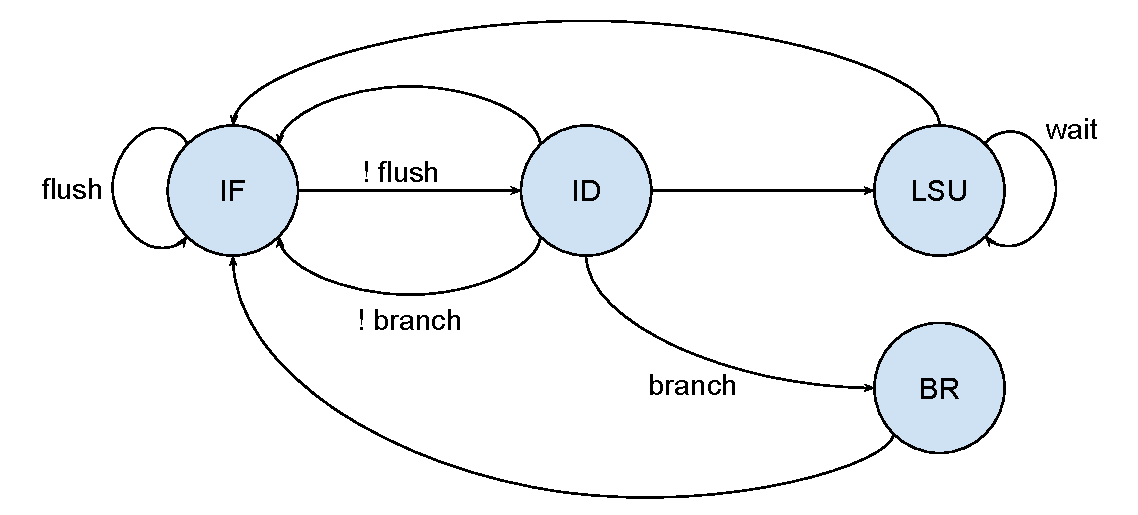
\includegraphics[width=\textwidth]{images/ri5cy-ppa.pdf}
	\caption{PPA extracted from the SystemC-PPA of the RI5CY core.}
	\label{fig:ri5cy-ppa}
\end{figure}

The important states depicted on the PPA correspond to the stages of the RI5CY pipeline. Even though the processor has a 4-stage pipeline, the register file was implemented as an external module, so there is no important state corresponding to this stage. Consequently, the behaviour of the signals that write to the register file is covered by the model and, therefore, by the generated property set. However, the register file functionality is not covered, and, as an independent module, it must have its own design and verification flow.

To illustrate the operations in the PPA of Fig.~\ref{fig:ri5cy-ppa}, consider an \textit{ADD} operation. It starts at the \textit{IF} state, and the first operation, represented by the edge from \textit{IF} to \textit{ID}, refers to when the instruction moves from the fetch stage to the decoder. The instruction fetching address is updated and a new request to the instruction memory is sent. The next operation starts in state \textit{ID}. In this operation, the add computation is done, and write back signals are set with the result and destination register address. Since all these steps happen in the same \textit{clock} cycle, they are part of the same operation. In addition, because the functionality of the register file is not part of the model, checking the correct write back signals is enough. Thus, there is no check on whether the right values are written to the registers or not. This behaviour would be covered by a separated property set for the register file module. Therefore, the ending state for this operation is already the \textit{IF} state as the execution of the instruction is done. The properties in the listing of Fig.~\ref{fig:ri5cy-if-id-micro-ppt-a} (a) and (b) show the two micro properties generated by DeSCAM for the those two operations from \textit{IF} to \textit{ID} and from \textit{ID} back to \textit{IF}.

\begin{figure}[htb]
    \begin{lstlisting}
    property IF;
    dependencies: no_reset;
    for timepoints:
        t_end = t+1;
    freeze:
        iaddr_at_t = iaddr@t,
        [...]
    assume:
        at t: IF;
        at t: !(flush_in_sig);
        at t: !((getEncType(instr_in_sig) == enc_j));
        at t: !((getEncType(instr_in_sig) == enc_i_j));
    prove:
        at t_end: ID;
        at t_end: encodedInstr == instr_in_sig_at_t;
        at t_end: iaddr == (4 + iaddr_at_t)[31:0];
        at t_end: instr_req_sig == (4 + iaddr_at_t)[31:0];
        at t_end: pcIf == pcIf_at_t;
        at t_end: prevInstr == prevInstr_at_t;
        during[t+1, t_end]: data_out_notify == false;
        during[t+1, t_end-1]: instr_req_notify == false;
        at t_end: instr_req_notify == true;
        during[t+1, t_end]: toRegsPort_notify == false;
    end property;\end{lstlisting}
    \caption{(a) Micro property describing operation from \textit{IF} stage to \textit{ID} stage of RI5CY PPA}
    \label{fig:ri5cy-if-id-micro-ppt-a}
\end{figure}

\begin{figure}[htb]
\ContinuedFloat
    \begin{lstlisting}
    property ID;
    dependencies: no_reset;
    for timepoints:
    t_end = t+1;
    freeze:
        encodedInstr_at_t = encodedInstr@t,
        [...]
    assume:
        at t: ID;
        at t: !((getInstrType(encodedInstr) == instr_unknown));
        at t: (getEncType(encodedInstr) == enc_r);
    prove:
        at t_end: IF;
        at t_end: encodedInstr == encodedInstr_at_t;
        at t_end: iaddr == iaddr_at_t;
        at t_end: pcIf == iaddr_at_t;
        at t_end: prevInstr == prevInstr_at_t;
        at t_end: toRegsPort_sig_dst == getRdAddr(encodedInstr_at_t);
        at t_end: toRegsPort_sig_dstData == getALUres(getALUfunc(readRegfile(fromRegsPort_sig_reg_file_01_at_t,...),getRs1Addr(),getRs2Addr());
        during[t+1, t_end]: data_out_notify == false;
        during[t+1, t_end]: instr_req_notify == false;
        during[t+1, t_end-1]: toRegsPort_notify == false;
        at t_end: toRegsPort_notify == true;
    end property;\end{lstlisting}
    \caption{(b) Micro property describing operation from \textit{ID} stage to \textit{IF} stage of RI5CY PPA}
    \label{fig:ri5cy-if-id-micro-ppt-b}
\end{figure}

For simplicity, all the instructions comprised by the ENC\_R, ENC\_I\_I, ENC\_U, ENC\_J, and ENC\_I\_J types have their operations represented by the \textit{IF-ID} and \textit{ID-IF} edges of the PPA in Fig.~\ref{fig:ri5cy-ppa}, although the properties generated for them are not the same. The \textit{load} and \textit{store} instructions for ENC\_I\_L and ENC\_S are represented by the four edges between states \textit{IF}, \textit{ID} and \textit{LSU}, including the wait edge. The \textit{branch} instructions of ENC\_B are represented by two paths. One includes the \textit{branch} edge and comprises the three operations between the states \textit{IF}, \textit{ID} and \textit{BR}. This path corresponds to the execution when a branch is taken. The second path includes the \textit{!branch} edge that corresponds to the operation for when a branch is not taken. In this case, the branch instruction has only two operations between the states \textit{IF} and \textit{ID}. Finally, the \textit{flush} edge represents the operation when the pipeline is flushed. The \textit{!flush} edge is the regular operation between \textit{IF} and \textit{ID} for all instructions.

Running the Pipeline Algorithm for the property set generated by DeSCAM will merge the micro and wait operations resulting in pipeline properties. The micro properties in Fig.~\ref{fig:ri5cy-if-id-micro-ppt-a} (a) and (b) will be merged into a single property describing the behaviour through all pipeline stages. This is shown in the listing of Fig.~\ref{fig:ri5cy-enc-r-ppt}.

\begin{figure}[htb!]
    \begin{lstlisting}
    property ENC_R;
    dependencies: 
        no_reset,
        in_out_constraints,
        no_unaligned_case,
        no_hwlp_case,
        instr_mem;
    for timepoints:
        t_id = t+1,
        t_ex = t_id+1;
    freeze:
        iaddr_at_t = iaddr@t,
        instr_in_sig_at_t = instr_in_sig@t,
        encodedInstr_at_t_id = encodedInstr@t_id,
        fromRegsPort_sig_reg_file_01_at_t = fromRegsPort_sig_reg_file_01@t_id,
        [...] //remaining register variables
        iaddr_at_t_id = iaddr@t_id;
    assume:
        at t: IF;
        at t: !(flush_in_sig);
        at t: !((getEncType(instr_in_sig) == enc_j));
        at t: !((getEncType(instr_in_sig) == enc_i_j));
        
        at t_id: !((getInstrType(encodedInstr) == instr_unknown));
        at t_id: (getEncType(encodedInstr) == enc_r);
    prove:
        at t_id: encodedInstr == instr_in_sig_at_t;
        at t_id: iaddr == (4 + iaddr_at_t)[31:0];
        at t_id: instr_req_sig == (4 + iaddr_at_t)[31:0];
        during[t+1, t_id]: data_out_notify == false;
        at t_id: instr_req_notify == true;
        during[t+1, t_id]: toRegsPort_notify == false;
        
        at t_ex: pcIf == iaddr_at_t_id;
        at t_ex: toRegsPort_sig_dst == getRdAddr(encodedInstr_at_t_id);
        at t_ex: toRegsPort_sig_dstData == getALUresult(getALUfunc(encodedInstr_at_t_id, readRegfile(fromRegsPort_sig_reg_file_01_at_t,getRs1Addr(),getRs2Addr()));
        during[t_id+1, t_ex]: data_out_notify == false;
        at t_ex: toRegsPort_notify == true;
    end property;\end{lstlisting}
    \caption{Pipeline property for ENC\_R instructions of RI5CY. This property is derived by merging the mirco properties in Fig.~\ref{fig:ri5cy-if-id-micro-ppt-a} (a) and (b).}
    \label{fig:ri5cy-enc-r-ppt}
\end{figure}

The property shown in Fig.~\ref{fig:ri5cy-enc-r-ppt} had some of its “\textit{freeze}” variables and function arguments omitted for simplicity reasons. The complete Pipeline Properties set can be found in \cite{descam}. The dependencies from lines 3 to 7 are the constraints valid for this property. The \textit{no\_reset} constraint is automatically added by DeSCAM and corresponds to a macro which defines that there is no incoming reset signal during the instruction execution. The \textit{instr\_mem} constraint refines the instruction memory protocol. The three other constraints disable RI5CY extension modules, such as the non-aligned memory access and \textit{hardware loop} extensions. In this case study, only the RISC-V 32 bits base instruction is modelled. The \textit{in\_out\_constraints} constrains some unused \textit{inputs} and \textit{outputs}, such as interruption signals, to be de-asserted. 

The two timepoints were added and updated according to the two micro properties from which the pipeline property was merged. The $t\_id$ timepoint corresponds to the commitments of the micro property in Fig.~\ref{fig:ri5cy-if-id-micro-ppt-a}a, and $t\_ex$ for the commitments in Fig.~\ref{fig:ri5cy-if-id-micro-ppt-b}b. In addition, the “\textit{freeze}” variables from lines 12 to 17 had also their names updated according to the corresponding micro property timepoint.

The assumptions from line 19 to 22 correspond to the assumptions in Fig.~\ref{fig:ri5cy-if-id-micro-ppt-a}a. The \textit{IF} macro state is refined to represent both \textit{ready to fetch} and \textit{empty pipeline} states. The other three assumptions determine that there should be no flushing and that the fetched instruction is not a \textit{jump}, what would change the processor behaviour already at $t\_id$. The assumptions in lines 24 and 25 are imported from Fig.~\ref{fig:ri5cy-if-id-micro-ppt-b}b. They specify that the instruction to be decoded is known and of the type ENC\_R. This determines the processor behaviour at $t\_ex$.

The commitments from lines 27 to 32 correspond to the operation \textit{IF-ID} from Fig.~\ref{fig:ri5cy-if-id-micro-ppt-a}a. As for the commitments from lines 34 to 38, they correspond to the operation \textit{ID-IF} from Fig.~\ref{fig:ri5cy-if-id-micro-ppt-b}b. By comparing the commitments of the micro properties and the merged property, it is possible to spot the inserted, deleted, and updated commitments by the merging steps of the pipeline algorithm. The helping macro functions are derived form the functions implemented in the ESL model, and they are fully automatically generated by DeSCAM, so no refinement is needed. The remaining signals and state macros are generated in a separate file and must be refined by the designer to match the signals and registers of the RTL implantation. 

In addition to the properties for all the instruction types, a micro property for the \textit{flush} edge describing the behaviour of the flushing operation is generated by DeSCAM, and it is refined by the Pipeline Algorithm. A property is also generated and refined for the operation when an unknown instruction is fetched. The assumptions for such property is shown in Fig.~\ref{fig:ri5cy-unknown-ppt}. An extra assumption, that is not part of the merging algorithm, is manually inserted, the \textit{illegal\_instr()} assumption. This assumption is only necessary in this special case study because not all instruction known to the RTL implementation are known to the ESL model. As a result, without this assumption, the property check tool would find a \textit{spurious} counter example with an instruction that is known to the RTL design, but not to the ESL model. In this case, the commitments would not be fulfilled, and the property would not hold. 

\begin{figure}[htb!]
    \begin{lstlisting}
    property UNKNOWN;
    [...]
    assume:
        at t: IF;
        at t: !(flush_in_sig);
        at t: !((getEncType(instr_in_sig) == enc_j));
        at t: !((getEncType(instr_in_sig) == enc_i_j));
        
        at t_id: (getInstrType(encodedInstr) == instr_unknown);
        //Manually added to exclude not covered instructions by ESL
        at t_id: illegal_instr (encodedInstr);
    prove:
    [...]
    end property;\end{lstlisting}
    \caption{Assumptions of the Pipeline Property that describes when a \textit{unknown} instruction is fetched.}
    \label{fig:ri5cy-unknown-ppt}
\end{figure}

Finally, a property with the assumptions such the ones shown in Fig.~\ref{fig:ri5cy-vacuous-ppt} is generated. This property assumes that the instruction fetched is not unknown but also not any of the known types. This results in an unreachable state. Therefore, the property checking tool classifies this property as a \textit{vacuous} pass, since no counter example nor witness can be found. In this context, witness means a valid example that is generated by the tool for which the property holds. 

\begin{figure}[htb!]
    \begin{lstlisting}
    property VACUOUS;
    [...]
    assume:
        at t: IF;
        at t: !(flush_in_sig);
        at t: !((getEncType(instr_in_sig) == enc_j));
        at t: !((getEncType(instr_in_sig) == enc_i_j));
        
        at t_id: !((getInstrType(encodedInstr) == instr_unknown));
        at t_id: !((getEncType(encodedInstr) == enc_r));
        at t_id: !((getEncType(encodedInstr) == enc_i_i));
        at t_id: !((getEncType(encodedInstr) == enc_i_l));
        at t_id: !((getEncType(encodedInstr) == enc_s));
        at t_id: !((getEncType(encodedInstr) == enc_b));
        at t_id: !((getEncType(encodedInstr) == enc_u));
        at t_id: !((getEncType(encodedInstr) == enc_j));
        at t_id: !((getEncType(encodedInstr) == enc_i_j));
    prove:
    [...]
    end property;\end{lstlisting}
    \caption{Assumptions of the Pipeline Property with an unreachable state where the fetched instruction is neither known nor unknown.}
    \label{fig:ri5cy-vacuous-ppt}
\end{figure}

\section{The \SSQED{} Properties}
\label{section:ri5cy-s2qed-ppt}

To make the set of pipeline properties complete, a set of \SSQED{} properties must be created. An overview about \SSQED{} can be seen in Sec.~\ref{section:s2qed}. The current section will present how a set of \SSQED{} properties was created to the RI5CY core.  Fig.~\ref{fig:ri5cy-enc-r-s2qed-ppt} shows a simplified \SSQED{} property for the instructions of type ENC\_R. This example is going to be used to analyse each part of a \SSQED{} property.

\begin{figure}[htb!]
    \begin{lstlisting}
    property S2QED_ENC_R;
    [...]
    for timepoints:
        t_if_i1 = t,
        t_id_i1 = t_if_i1+1,
        t_wb_i1 = t_id_i1+1,
        t_done_i1 = t_wb_i1+1,
        
        t_if_i2 = t,
        t_id_i2 = t_if_i2+1..5 waits_for (CPU2_STALL == 0 && cpu2/id_ready == 1),
        t_wb_i2 = t_id_i2+1,
        t_done_i2 = t_wb_i2+1;
        [...]
    assume:
        // constraints on CPU1
        at t_if_i1: start_state && empty_pipeline;
        during [t_if_i1 + 1, t_done_i1]: cpu1/instr_rdata_i == 32'h13;
        // same instruction for IUV
        at t: !(getInstrType(cpu1/instr_rdata_i) == instr_unknown); 
        at t: getEncType(cpu1/instr_rdata_i) == enc_r;
        at t: cpu1/instr_rdata_i == cpu2/instr_rdata_i;
        at t: cpu1/instr_addr_o == cpu2/instr_addr_o;
        // QED consistent registers
        at t_wb_i2: foreach r in 0..31: 
        (regfile_i1_at_t_wb_i1[r] == REGISTER_CPU2(r) || (cpu2/regfile_we_wb && cpu2/regfile_waddr_fw_wb_o == resize(r,6))); 
        end foreach;
        at t_wb_i2: foreach r in 0..31: 
        (!cpu2/regfile_we_wb || cpu2/regfile_wdata == regfile_i1_at_t_wb_i1[r]); 
        end foreach;
        //Flushing
        during [t_if_i2, t_id_i2]: CPU2_NO_FLUSH_STATE;
        //I/O should be the same (no stalling)
        at t: CPU2_STALL == 0 && cpu2/id_ready == 1 && cpu2/if_stage_i/if_ready == 1;
    prove:
        // PC register
        at t_id_i2: cpu2/pc_if == cpu1_pcIf_at_t_id_1;
        // general registers
        at t_done_i2: cpu2/id_stage_i/registers_i/riscv_register_file_i/mem == regfile_i1_at_t_done_i1;
    end property;\end{lstlisting}
    \caption{\SSQED{} property for instructions of type ENC\_R.}
    \label{fig:ri5cy-enc-r-s2qed-ppt}
\end{figure}

The \textit{dependencies} field was omitted because the constraints should follow the same construction idea as for the pipeline properties. For the timepoints, however, a major difference can be noticed; there are two set of time variables, one for each instance of the processor, \textit{cpu1} and \textit{cpu2}. Starting with \textit{cpu1}, the reader will notice that there are more timepoints than it would be expected if compared with the pipeline properties. This happens because the \SSQED{} focus on the consistency of the two CPU instances, rather than the result of the instruction operation. Consequently, checking the consistency between the register files demands an additional timepoint that relates to the time when the result is written back to the destination register. This additional timepoint corresponds to $t\_done$. Furthermore, the $t\_ex$ timepoint, which corresponds to the time when the ALU executes the operation and also when the write back signals are set, was renamed to $t\_wb$ to reflect the emphasis on the write back.

The assumptions start with the restrictions for \textit{cpu1}, stating that it is \textit{ready to fetch} at $t\_if$, it has an \textit{empty pipeline}, and that the instructions after the IUV are only \textit{nop}’s. This last assumption is not a requirement for the correctness of the model, instead it aims to reduce the complexity for the SAT-solving tool. Since the \SSQED{} properties have two independent instances executing, the complexity for the property checking tool and therefore the time needed for proving each property grows rapidly.

The next assumption refers to the IUV that must be of type ENC\_R. Both CPU instances fetch the same instruction at $t\_if$. In addition, the \textit{output} address must also be the same. This assumption is important to be able to prove the consistency of the PC register. Next, the property assumes that the CPU instances are consistent at $t\_wb$. Finally, the last two assumptions refer to the \textit{cpu2} and requires that there is no flushing between $t\_if$ and $t\_id$, so that the IUV is not flushed, and that \textit{cpu2} is \textit{ready to fetch} at $t\_if$ when the IUV is fetched.

The two commitments are proving that the PC register of both CPU instances are consistent at $t\_id$, and that the register files are consistent at $t\_done$.

\subsection*{QED Consistency}

The base concept for QED consistency is presented in Sec.~\ref{section:s2qed} with emphasis on instructions of register type. However, the RTL implementation in this case study has an important particularity that requires further elaboration on consistency. The RI5CY core has two write back ports to the register file. One port for write back from the ALU, which is used for arithmetic and logic operations, and the other write back port is used by the LSU for loading data from the memory.

These two write back ports allow data to be written to two registers in the register file at the same time. Consider a scenario when there is a \textit{load} instruction followed by an \textit{add} instruction in \textit{cpu2}, and that the \textit{add} is the IUV. By the time the data is loaded from the memory, it is possible that the result from the \textit{add} operation is also available to write back. As a result, both loaded data from memory and add result will be written to their respective destination register at the same time. This would cause the \SSQED{} property to fail on the commitment of consistent register files at $t\_done$ because \textit{cpu1} will only write the add result from the ALU to its register file.

In order to deal with this simultaneous write back, the \textit{qed\_consistency\_registers} in Eq.~\ref{eq:consistency-register} in Sec.~\ref{section:s2qed} is modified to Eq.~\ref{eq:new-consistency-register}. $C$ and $U$ refer to the constrained \textit{cpu1} and unconstrained \textit{cpu2} respectively. $r^{t_{wb}}$ corresponds to the value of a specific register in the register file at $t\_wb$, $i^{t_{wb}}_r$ is the \textit{input} value to be written to register $r$ at $t\_wb$, and $w^{t_{wb}}_r $ is the write enable signal to register $r$ at $t\_wb$.

\begin{equation}
    qed\_consist\_reg := \bigwedge_{r \in U} \left((r^{t_{wb}}_U = r^{t_{wb}}_C) \lor w^{t_{wb}}_r\right) \land \bigwedge_{r \in U} \left(w^{t_{wb}}_r \rightarrow (i^{t_{wb}}_r = r^{t_{wb}}_C)\right)
    \label{eq:new-consistency-register}
\end{equation}

The extended qed\_consist\_reg of Eq.~\ref{eq:new-consistency-register} specifies that at $t\_wb$ either each register in \textit{cpu2} holds the same value as its corresponding register in \textit{cpu1}, or there is a write back for that register. If there is a write back to that register, the \textit{input} value to be written to the register is the same value that the corresponding register in \textit{cpu1} holds at $t\_wb$. This QED consistency is shown in lines 24 to 29 of the property in Fig.~\ref{fig:ri5cy-enc-r-s2qed-ppt}.

This QED consistency assumption of ENC\_R instructions is also valid for the ENC\_U, ENC\_J and ENC\_I\_J, as they use the same write back port from the ALU to write to the register file at $t\_wb$. The remaining instructions considered for this case study have the same previous QED consistency because they do not check the whole register file in the commitments at $t\_done$.

The \textit{load} instructions will check the consistency of the destination register after write back because the case of simultaneous access is covered by the properties for the instructions that uses the ALU write back port. The ENC\_S instructions do not need to check the register files as they do not write to the registers. As shown in Fig.~\ref{fig:ri5cy-enc-s-s2qed-ppt}, it only checks PC and the consistency of the data memory output signals at $t\_ex$. The branch instructions will check the consistency of the PC register, \textit{branch decision} signal, and instruction fetching address for the case when the branch is taken, Fig.~\ref{fig:ri5cy-enc-b-s2qed-ppt-taken}, or simply the PC and \textit{branch signal} consistency for the case when the branch is not taken, Fig.~\ref{fig:ri5cy-enc-b-s2qed-ppt-not-taken}. The complete set of \SSQED{} properties is found in \cite{descam}.

\begin{figure}[htb!]
    \begin{lstlisting}
    property S2QED_ENC_S;
    [...]
    prove:
        // PC register
        at t_id_i2: cpu2/pc_if == cpu1_pcIf_at_t_id_1;
        
        // Data Memory Output
        at t_ex_i2: cpu2/data_req_o == data_req_at_ex_i1;
        at t_ex_i2: cpu2/data_we_o == data_we_at_ex_i1;
        at t_ex_i2: cpu2/data_addr_o == data_addr_at_ex_i1;
        at t_ex_i2: cpu2/data_wdata_o == data_wdata_at_ex_i1;
    end property;\end{lstlisting}
    \caption{Commitments of \SSQED{} property for ENC\_S instructions.}
    \label{fig:ri5cy-enc-s-s2qed-ppt}
\end{figure}

\begin{figure}[htb!]
     \centering
     \begin{subfigure}[b]{\textwidth}
         \begin{lstlisting}
    property S2QED_ENC_B_TAKEN;
    [...]
    prove:
        // PC register
        at t_id_i2: cpu2/pc_if == cpu1_pcIf_at_t_id_1;
        at t_done_i2: cpu2/pc_if == cpu1_pcIf_at_t_done_1;
        
        // Branch Result
        at t_ex_i2: cpu2_flush_sig == cpu1_flush_sig_at_t_ex_i1;
        
        // Instr Memory Output
        at t_ex_i2: cpu2/instr_addr_o == instr_addr_at_t_ex_i1;
    end property;\end{lstlisting}
         \caption{Commitments of \SSQED{} property for ENC\_B instructions when the branch is taken.}
         \label{fig:ri5cy-enc-b-s2qed-ppt-taken}
     \end{subfigure}
     \hfill
     \begin{subfigure}[b]{\textwidth}
         \begin{lstlisting}
    property S2QED_ENC_B_NOT_TAKEN;
    [...]
    prove:
        // PC register
        at t_id_i2: cpu2/pc_if == cpu1_pcIf_at_t_id_1;
        
        // Branch Result
        at t_ex_i2: cpu2_flush_sig == cpu1_flush_sig_at_t_ex_i1;
    end property;\end{lstlisting}
         \caption{Commitments of \SSQED{} property for ENC\_B instructions when the branch is not taken.}
         \label{fig:ri5cy-enc-b-s2qed-ppt-not-taken}
     \end{subfigure}
        \caption{Commitments of \SSQED{} property for ENC\_B instructions for both cases when the branch is (a) taken and (b) not taken.}
        \label{fig:ri5cy-enc-b-s2qed-ppt}
\end{figure}
\newpage
% ----------------------------------------------------------
% Results
% ----------------------------------------------------------
\chapter{Experimental Results}
\label{chapter:results}

In Chapter \ref{chapter:ri5cy}, the ESL model for the RI5CY processor core and the generation and refinement of a complete set of properties, including the pipeline and \SSQED{} properties, are presented. The current chapter discusses the experimental results for the ESL model including a comparison with the RTL implementation. In addition, the experiments analyse the property generation and property checking process. Finally, a comparison with the bottom-up verification flow is discussed.

Table~\ref{tab:esl-rtl-comp} provides a comparison between the ESL model and the RTL implementation. As expected, given the higher abstraction level of the ESL, the number of \textit{Lines of Code}~(LoC) is much lower for the ESL than the RTL. The LoC counting for the ESL includes the RI5CY CORE and the Register File modules, since the register file is part of the core in the RTL. The RTL modules for extensions that are not comprised by the ESL were not taken into consideration for counting the lines. However, there is still code present at the considered RTL modules referring to these extensions, and also to decoding and executing all the instructions not implemented by the ESL. The results also include an estimated effort to implement the ESM model. This measure comprises the implementation of the RI5CY CORE and the Memory interface (IMEM), and it includes the effort to understand the pipeline behavior, i.e. pipeline stages and how each instruction is executed through them, and the \textit{flushing} behaviour. There is no measure of approximated effort for the RTL model because an existent implementation was used in the case study.  

\begin{table}[htb!] 
	\centering 
	\caption{LoC and Simulation results for the ESL and RTL model.} 
	\label{tab:esl-rtl-comp}
	\begin{tabular}{p{5cm} c c} 
		  &  \textbf{ESL} & \textbf{\SSSAY{RTL}} \\     
		\hline	
		Lines of Code  & 856 & XX \\
		Design Effort & 2 person weeks & - \\
		\hline
		\textbf{Simulation Time} (s) & & \\
		\hline
		Prime Numbers  &  1.44 & XX \\
		Fibonacci  &  0.27 & XX \\
		Bubble Sort  &  0.34 & XX \\
	\end{tabular} 
\end{table}

The simulation results presented in Table~\ref{tab:esl-rtl-comp} refer to the simulation of three computation-heavy programs for the ESL and RTL models. The first program computes ten prime numbers greater than 1000. The second one computes 1000 numbers of the Fibonacci sequence. The third program implements the execution of the \textit{Bubble Sort} algorithm to sort an array of 50 integers in ascending order. To consider the worse-case execution time for \textit{Bubble Sort}, the array is initially sorted in descending order.

The simulations were conducted on an Intel Core~i7 8550U @~1.80\,GHz with 8\,GB of RAM. All the simulations were much faster for the ESL model, as expected. This also reflects the higher abstract implementation of the system-level compared to the RTL implementation.

The same environment was used to run the \textit{DeSCAM} tool for the implemented ESL model to generate the set of micro properties. The results are presented in Table~\ref{tab:micro-ppt-results}. \textit{DeSCAM} takes approximately 28\,s to parse the ESL model and generate the micro properties set with a total of 21 properties. Considering only the lines of code for the generated properties, the count is 661\,LoC. When the generated macros to be refined by the designer are considered, the new count is 925\,LoC. \textit{DeSCAM} also generates a file with macros of functions that correspond to the functions implemented at the ESL model. For this experiment, the generated file has 201 LoC, but the designer does not need to do any refinement for these macro functions.  

\begin{table*}[htb!] 
	\centering 
	\caption{Results for micro properties generated by \textit{DeSCAM} from the RI5CY ESL model.} 
	\label{tab:micro-ppt-results}
	\begin{tabular}{p{6cm} c } 
		\multicolumn{2}{c}{\textbf{Micro Properties Set}} \\  
		\hline	
		Time to generate properties  &  27.4 s  \\
		Number of properties  &  21 \\
		LoC (properties only)  &  661 \\
		LoC (properties \& macros)  &  925\\
	\end{tabular} 
\end{table*}

The next step is the creation of the set of pipeline and \SSQED{} properties. Table~\ref{tab:pipe-s2qed-ppt-resutls} shows the estimated effort for applying the pipeline algorithm to create the merged properties, and the estimated effort to create the \SSQED{} property set. Even though the \SSQED{} properties are not created from any automatically generated properties, they are not build from scratch. The number of properties needed is guided by the merged pipeline properties, i.e. for each merged property corresponding to a type of instruction, a \SSQED{} should be written. In addition, the refined state macros, e.g. \textit{ready to fetch} and \textit{empty pipeline}, and the generated function macros can be reused. The effort shown for the pipeline property set takes into consideration the application of the pipeline algorithm to merge the micro properties, but not the macros refinement.The estimated effort to refine the macros is 1\,\textit{person\,week}. This effort is considerably large because the RI5CY user manual \cite{manual-ri5cy} does not have detailed specification and much of the effort went towards extracting information from the RTL implementation.

Table~\ref{tab:pipe-s2qed-ppt-resutls} also shows the resulting number of merged and \SSQED{} properties, and the number of Lines of Code for both. The difference on the number of properties between the property sets occurs because the \SSQED{} set does not include the \textit{reset}, \textit{vacuous}, \textit{flush} and \textit{unknown} properties. In addition, there is only one \SSQED{} property for both \textit{jump} instructions. Regarding the lines of code, only the properties were taken into consideration, since the macros and functions are common for both sets.

\begin{table*}[htb!] 
	\centering 
	\caption{Results comparison between the Pipeline and \SSQED{} properties sets.} 
	\label{tab:pipe-s2qed-ppt-resutls}
	\begin{tabular}{p{5cm} c c} 
		  &  \textbf{Pipeline} & \textbf{\SSQED{}} \\     
		\hline	
		Effort  &  5 person hours & 1 person week \\
		Number of Properties  &  13 & 8 \\
		Lines of Code  &  634 & 502 \\
	\end{tabular} 
\end{table*}

Finally, the resulting property set was checked for the RTL design. The property checking was conducted with the commercial property checker OneSpin~360~DV-Certify \texttrademark{} running on an Intel Xeon~E5-2637~v4  @~3.50\,GHz with 96\,GB of RAM. Table~\ref{tab:pipe-s2qed-check-resutls} shows the checking time and memory used results both pipeline and \SSQED{} property sets.

\begin{table*}[htb!] 
	\centering 
	\caption{Results for checking time and memory used for Pipeline and \SSQED{} properties sets.} 
	\label{tab:pipe-s2qed-check-resutls}
	\begin{tabular}{lcccc}
          & \multicolumn{2}{c}{\textbf{Pipeline Properties}} & \multicolumn{2}{c}{\textbf{\SSQED{} Properties}} \\
          \hline
         Instruction Type & Time (h:m) & Mem.(GB) & Time (h:m) & Mem.(GB)  \\
          \hline
        ENC\_R & 00:23 & 9.7 & 1:37 &  21.4  \\
        ENC\_I\_I & 00:19 & 9.4 & 11:27 &  26.5\\
        ENC\_B taken  & 00:02 & 8.8 & 1:12 & 19\\
        ENC\_B not taken & 00:10 & 9.4 & 1:07 &  24  \\
        ENC\_J & 00:03 & 8.7 & - &  -  \\
        ENC\_I\_J & 00:07 & 9.7 & - &  -  \\
        ENC\_JUMP & - & - & 10:27 &  23  \\
        ENC\_I\_L & 1:00 & 23.3 & \SSSAY{X} & \SSSAY{X}  \\
        ENC\_S & 00:08 & 12.2 & 4:15 &  24.9  \\
        ENC\_U & 00:14 & 9.4 & 9:02 & 20.7  \\
        RESET & < 0:01 & 1.1 & - &  -  \\
        FLUSH & 00:10 & 7.8 & - &  -  \\
        UNKNOWN & < 0:01 & 5.5 & - &  -  \\
        VACUOUS & < 0:01 & 0.9 & - &  -  \\
\end{tabular}
\end{table*}

The longer checking time for the pipeline properties occurred for the \textit{ENC\_I\_L} instruction type. This is justified by the inserted bounded wait of five cycles for the data memory. The \textit{ENC\_I\_L} is followed by \textit{ENC\_R} and \textit{ENC\_I\_I} types. This is because these types comprise the greater number of associated instructions, for instance all the arithmetic, logic, and logic shift instructions.

The results for the \SSQED{} property set were obtained with some constraints regarding the number of registers considered for the checker. All the register fields of the IUV were restricted to be lower than five, i.e. the instruction will access the four first register of the register file. In addition, the bounded wait for \textit{load} and \textit{store} instructions were limited to three instead of five. These restrictions were applied to reduce the complexity for the property checker. This complexity issue is evidenced when comparing both checking time and memory used between the \SSQED{} properties set with the pipeline properties set. Both measurements are much higher for the \SSQED{} set than for the pipeline set for all instruction types.

Even though the checking time required for making a property hold can be of several minutes, or even hours, the property checking tool needs much less to find a \textit{bug}. A \textit{bug} was inserted on the forwarding mechanism of the processor core. This type of error is only detected by the \SSQED{} property set, since \textit{forwarding} only happens for specific program contexts where instructions at different pipeline stages interact. The property checking tool needed 4\,min\,and\,58\,s to find a counter-example for an \textit{ENC\_I\_L} \SSQED{} property, and only 2\,min\,and\,6\,s for an \textit{ENC\_R} \SSQED{} property. Similarly, a \textit{bug} was inserted on the operand signals from the register file to the ALU. This type of \textit{bug} is considered single-instruction error because it can be spotted by properties for IUV executing in an empty pipeline. Thus, the property checking tool found a counter-example for an \textit{ENC\_I\_L} pipeline property in 1\,min\,and\,36\,s and for an \textit{ENC\_R} pipeline property in 15\,s.

For means of comparison, the experiments included the creation of pipeline properties in a \textit{bottom-up} approach. This property set was created strictly from the behaviour extracted from the RTL design, and it is not part of the PDD flow. In this case, the properties were created from the ground up based on the implemented RTL and its signals. No automatically generated macros or functions were used. One property for each instruction was created. However, macros were employed to unify the properties of each type of instruction, and each instruction property just instantiated the corresponding macro, e.g. all arithmetic and logic instructions of R-type and I-type use the same property macro. This use of macros resulted in eight property macros.

Table~\ref{tab:bottom-up-ppt-resutls} shows the experimental results of the bottom-up constructed pipeline properties in comparison to the pipelined properties merged from the micro properties in the PDD flow. The results indicate a much larger effort to create the properties from bottom-up than with the PDD flow using an ESL model. The effort shown in the "Pipeline PDD" combines the effort for merging the properties and refining the macros in the PDD flow. The lines of code includes the code for both properties and refined macros. For the bottom-up constructed properties, the number of properties represent the number of property macros. It has less properties macros than pipeline properties because it does not have properties for unknown instruction and \textit{flushing}. In addition, all R-type and I-type arithmetic and logic instructions are described by the same macro property. The same happens for the \textit{jal} and \textit{jalr} instructions. 

\begin{table*}[htb!] 
	\centering 
	\caption{Results from comparison between pipeline properties created in a bottom-up approach and pipeline properties generated using the merging algorithm within the PDD flow.} 
	\label{tab:bottom-up-ppt-resutls}
	\begin{tabular}{p{5cm} c c} 
		  &  \textbf{Botton-up} & \textbf{Pipeline (PDD)} \\     
		\hline	
		Effort  &  1 person month &  8 person days\\
		Number of Properties  &  8 & 13 \\
		Lines of Code  & 879  &  834\\
	\end{tabular}
\end{table*}

Table~\ref{tab:bottom-up-check-resutls} shows the results for the running checking time and the memory used for each property. Since each instruction has its own property, a direct comparison of checking time is not possible as the pipeline properties from the PDD flow are grouped per type. Nonetheless, the total time for checking all the instructions can be compared. The checking time for the PDD pipeline properties is \SSSAY{X} minutes, and \SSSAY{X} minutes for the bottom-up properties.

\begin{table*}[htb!] 
	\centering 
	\caption{Checking time and memory used results for pipeline properties created on a bottom-up approach.} 
	\label{tab:bottom-up-check-resutls}
		\begin{tabular}{p{4cm}cc}
          \multicolumn{3}{c}{\textbf{Bottom-up Pipeline Properties}} \\
          \hline
         Instruction Type & Time (h:m) & Mem.(GB)  \\
          \hline
        add     & \SSSAY{XX} & \SSSAY{XX}  \\
        sub    &  &  \\
        sll     &  &  \\
        slt    &  &  \\
        sltu    &  &  \\
        xor    &  &  \\
        slr    &  &  \\
        sra    &  &  \\
        or    &  &  \\
        and    &  &  \\
        addi    &  &  \\
        slti    &  &  \\
        sltiu    &  &  \\
        xori    &  &  \\
        ori    &  &  \\
        andi    &  &  \\
        slli    &  &  \\
        srli    &  &  \\
        srai    &  &  \\
        beq taken    &  &  \\
        beq not taken     &  &  \\
        bne taken    &  &  \\
        bne not taken    &  &  \\
        blt taken    &  &  \\
        blt not taken    &  &  \\
        bge taken    &  &  \\
        bge not taken    &  &  \\
        bltu taken    &  &  \\
        bltu not taken    &  &  \\
        bgeu taken    &  &  \\
        bgeu not taken    &  &  \\
        jal    &  &  \\
        jalr    &  &  \\
        lb    &  &  \\
        lh    &  &  \\
        lw    &  &  \\
        lbu    &  &  \\
        lhu    &  &  \\
        sb    &  &  \\
        sh    &  &  \\
        sw    &  &  \\
        lui    &  &  \\
        auipc    &  &  \\
        reset    &  &  \\
        
\end{tabular}
\begin{tabular}{lcc}
          \multicolumn{3}{c}{\textbf{Bottom-up Pipeline Properties}} \\
          \hline
         Instruction Type & Time (h:m) & Mem.(GB)   \\
          \hline
        ENC\_R & 00:42 &    \\
        ENC\_I\_I & 00:19 &  \\
        ENC\_B taken  & 00:02 & \\
        ENC\_B not taken & 00:10 &    \\
        ENC\_J & 00:03 &    \\
        ENC\_I\_J & 00:07 &    \\
        ENC\_I\_L & 1:00 &   \\
        ENC\_S & 00:08 &    \\
        ENC\_U & \SSSAY{X} &   \\
        RESET & < 0:01 &    \\
\end{tabular}
\end{table*}
\newpage
% ----------------------------------------------------------
% Conclusion
% ----------------------------------------------------------
\chapter{Conclusion}
\label{chapter:conclusion}

In this work, an algorithm for property generation for pipelined processors was presented. This algorithm extends a Property-First design approach, called Property-Driven Design (PDD) methodology, to improve its applicability for pipelined processors. The methodology is based in a property checking formal verification method. For a given SystemC-PPA description of a processor, a set of properties is generated, and the proposed Pipeline Algorithm is used to create a set of pipeline properties to be later refined. The refinement of the property set is done simultaneously with the implementation of the RTL processor. At the end of the design flow, when a complete set of properties hold for the implemented RTL, an ESL model that is sound to the RTL implementation is obtained. Having a trusted system-level model allows its usage as a reference model the same manner as the RTL.

A case study for a RISC-V processor implementation, the RI5CY core, was performed in this work. A SystemC-PPA description for the base instruction set of the core was implemented, and a set of properties generated from it using the \textit{DeSCAM} tool. The Pipeline Algorithm was employed to merge the properties into a set of pipeline properties. For completeness, a set of \SSQED{} properties was written for the core as well. This property set was refined according to the signals and control registers of the given RTL processor implementation until all the properties hold. The experimental results show a \textit{speedup} of approximately 144~times from the simulation at ESL to the RTL simulation. The estimated ESL design effort was only 2~person~weeks, and the effort estimated for applying the Pipeline Algorithm and completely refine the property set was 8~person~days. For means of comparison a set of properties was created directly from the RTL implementation in a \textit{bottom-up} approach, and the estimated effort for creating property set was 1~person~month.

For future work, the proposed algorithm can be implemented and included into the DeSCAM tool so the process for generating properties for pipelined processors can be completely automatized. In the same manner, the generation of the \SSQED{} property set can be also implemented so a complete set of properties can automatically generated and then refined.
\newpage
% \input{chapters/6_ausblick.tex}
% \newpage

\backmatter
\listoffigures 
\listoftables
% \listoflistings

%%%%%%%%%%%%%%%%%%%%%%%%%%%%%%%%%%%%%%%%%%%%%%%%%%%%%%%%%%%%%%%%%%%%%%%%
% Choose your Bibtex Style File (here alphadin.bst) and references.
% Hint: For references make a local link refs2 to our jabref 
% directory "/import/jabref/refs2.bib"
%%%%%%%%%%%%%%%%%%%%%%%%%%%%%%%%%%%%%%%%%%%%%%%%%%%%%%%%%%%%%%%%%%%%%%%%

%%%%%%%%%%%%%%%%%%%%%%%%%%%%%%%%%%%%%%%%%%%%%%%%%%%%%%%%%%%%%%%%%%%%%%%%
% \bibliographystyle{alphadin}
\bibliographystyle{plain}
% \bibliography{refs3}
\bibliography{myrefs} %I added this
% \bibliography{myrefs}
% \input{mybiblio}%\todo{use bibtex!}
%%%%%%%%%%%%%%%%%%%%%%%%%%%%%%%%%%%%%%%%%%%%%%%%%%%%%%%%%%%%%%%%%%%%%%%%

%%%%%%%%%%%%%%%%%%%%%%%%%%%%%%%%%%%%%%%%%%%%%%%%%%%%%%%%%%%%%%%%%%%%%%%%
% Curriculum Vitae
%%%%%%%%%%%%%%%%%%%%%%%%%%%%%%%%%%%%%%%%%%%%%%%%%%%%%%%%%%%%%%%%%%%%%%%%
%\selectlanguage{german}
%\input{cv.tex}
%\selectlanguage{english}

\end{document}
